\documentclass[a4paper,11pt,twoside]{pads-thesis}

%%%%% PACKAGES USED SORTED ALPHABETICALLY  %%%%%
\usepackage[toc,page]{appendix} % support appendices
\usepackage{csquotes} % handles quotes automatically
\usepackage{hyperref} % allows autoref/hyperlinks/etc.
\usepackage{amsmath}
\usepackage{stmaryrd}


%%%%% PADS TEMPLATE SETTINGS %%%%%
\renewcommand{\gTitle}{Estimating Probabilities for Realizations of Uncertain Event Data}
\renewcommand{\gAuthor}{Bianka Bakullari}
\renewcommand{\gStudentID}{363085}
\renewcommand{\gHeader}{Master's Thesis}
\renewcommand{\gSupervisor}{
    Marco Pegoraro M.Sc.}
\renewcommand{\gExaminer}{Prof. Wil van der Aalst \\ 
	Prof. Joost-Pieter Katoen }
\renewcommand{\gInstitution}{i9 Process and Data Science (PADS) Chair, RWTH Aachen University}
%\renewcommand{\gRegDate}{YYYY-MM-DD}
%\renewcommand{\gSubDate}{YYYY-MM-DD}

%%%%% AUTOREF %%%%%
\renewcommand{\sectionautorefname}{Section}

\begin{document}
%%% Title page
\pagenumbering{roman}

\gTitlePage
%\pagestyle{plain}
%%% TOC

%\begin{abstract}
\chapter*{Abstract} \addcontentsline{toc}{chapter}{Abstract}
Process mining is a research discipline that deals with the analysis of process related event data by discovering process models, checking conformance between real process runs and normative models, and improving the performance of processes in many aspects.
Most approaches assume that for each process instance a unique trace of performed activities can be extracted.
In uncertain event logs, however, many event attributes do not contain unique values, thus leading to many possible traces that might have been executed.
In this work, we exploit the information enclosing event data with explicit description of uncertainty, and obtain probability estimates for the realizations of uncertain process instances.
We motivate the importance of obtaining such estimates using conformance checking examples, and we also validate the obtained values on an example by means of the Monte Carlo simulation method.
Moreover, we introduce a new method for obtaining all possible orderings of events belonging to the same uncertain process instance, and analyze its performance against the baseline method both theoretically and experimentally.
 \label{chap: abstract}
%\end{abstract}

\tableofcontents

%\setcounter{page}{1}
\cleardoublepage
%%% Begin document
\pagestyle{fancy}
\pagenumbering{arabic}

\chapter{Introduction} \label{chap:intro}
Process mining \cite{pm} is an ever-growing research field that provides a number of methods and algorithms aiming to help analyze and gain insight over processes.
Processes consist of sets of activities that are performed over some time span indicating the steps that were executed to complete a specific task or goal.
An ever-increasing number of businesses use \textit{Process-Aware Information Systems (PAISs)} as software tools to aid them in generating and managing digital records for every process-related step that is performed.
This information can then be extracted in the form of an \textit{event log}, a database that contains a number of unique events that were executed as part of particular runs of the process.
An event might be enclosed with information indicating the specific activity and the resource that performed it, the time it was executed, and other additional attributes.

The main entity in the process-view of the provided event data are the \textit{process instances}.
Each process instance is identified through a unique \textit{case ID}, an event attribute that assigns each event to a unique process run.
For this reason, we often use the terms case and process instance interchangeably.
Each case has a corresponding set of events that were executed in some order and during which particular activities were performed.
The \textit{activity} attribute enables obtaining the activity that was performed from each event from the event set belonging to any process instance, whereas the \textit{timestamp} attribute enables ordering the performed activities into a chronological sequence, called \textit{trace}.
The case ID, activity and timestamp are the three necessary event attributes that provide the \textit{control-flow} perspective of any process.
While each process instance has a corresponding timely ordered sequence of events, it is the projection of these events onto the corresponding executed activities, the \textit{traces}, which yield meaningful information.
Assuming that the data was recorded correctly, the traces are real examples of process runs, possibly containing many reoccurring patterns.
The more data are available, the higher the number of real examples from which one can conclude what the ``real'' process looks like.
Using data-driven algorithms that transform given multisets of traces into graphs and models that are as understandable, accurate and precise as possible is the main goal of \textit{process discovery}.
Discovery algorithms typically produce models in the form constructs such as Petri Nets, BPMN models, and Process Trees.
Many commercial tools, however, produce models in the form of  \textit{Directly-Follows-Graphs (DFGs)}.
In DFGs, nodes stand for recorded activities, whereas directed arcs connect activity pairs whenever they were recorded happening consecutively.
Another important task in process mining is \textit{conformance checking}, whose aim is to compare recorded with expected or prescribed process behavior.
A challenge in conformance checking is discovering methods that are both efficient and robust in measuring at what degree the recorded process runs conform to the allowed behavior indicated by a prescriptive model.
Process mining methods provide insight and diagnostics derived from real event data.
Taking active decisions to change the process based on that knowledge may lead to overall improved processes which may be more efficient, have lower risks, ensure greater customer satisfaction, reduce bottlenecks, and prevent fraud.\\
The quality of the insights that process mining methods provide depends, however, on the quality of the recorded data.
The data may be noisy, containing spurious, inconsistent or missing values.
If the inaccurate or noisy values are infrequent, this problem is usually addressed by removing the affected records from the data that will be later used for analysis.
If on the other hand, the inaccuracies are frequent and pervasive, filtering methods may cause too much information loss and make the data unusable.
In our work, we assume that event data is \textit{uncertain}, in the sense that the event attributes do not always contain unique values.
This uncertainty is \textit{explicit}, since events are enclosed with a formal description of the possible values of the affected attributes.
The framework we use for classifying and handling event data with explicit uncertainty was first introduced in \cite{mining}.
We distinguish two types of uncertainty:
\begin{itemize}
\item \textit{Strong uncertainty}: a set or a range of possible attribute values is known, but the information regarding their distribution is missing or is unobtainable. 
\item \textit{Weak uncertainty}: both the possible values and their corresponding distribution are at disposal.
\end{itemize}
%
%
%
%
%
\begin{figure}[htp]
  \centering
 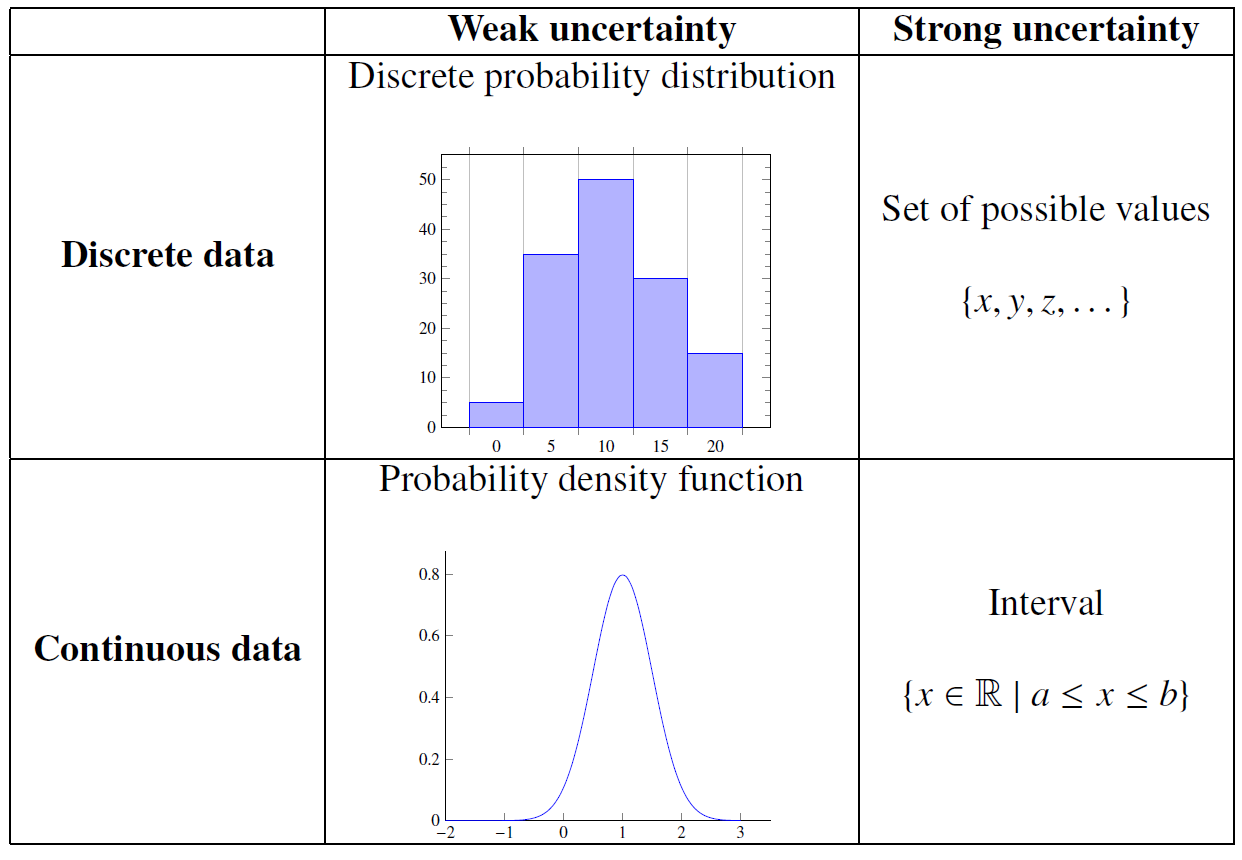
\includegraphics[width=12cm]{figures/unctypes.png}
	\caption{The four different types of uncertainty \cite{conformance}.}
	\label{fig: uncertainty types}
\end{figure}
%
%
%
%
%
Fig. \ref{fig: uncertainty types} from \cite{conformance} summarizes these types of uncertainty both for discrete and continuous domains.
There are various reasons which might cause uncertainty in the recorded event data.
Recordings might be prone to human errors if the data is inserted manually.
On the other hand, software errors might affect the data in unpredictable ways.
Under such circumstances, the data may display many quality issues including incorrectness, ambiguity, inconsistency, coarseness and so on.
Such factors, however, only \textit{imply} uncertainty in the data.
Describing uncertainty explicitly may be done straightforwardly or with the help of a domain expert.
If the recorded timestamps are too coarse, e.g. only the date but not the exact time is recorded, then the uncertain timestamps correspond to a time interval whose extremes are the start and end of the corresponding day.
If the executed activity of a particular event is not recorded, then knowing the resource who executed that event might indicate that the possible activities correspond to the tasks usually performed by that resource.
The uncertainty accompanying recorded measurements might also be explicit beforehand.
For instance, sensors might have an error model that follows a normal distribution around the measured value.
In this work, we focus on the uncertainty affecting two of the control-flow attributes: activity and timestamp.
Additionally, we account for events whose execution is uncertain, which we call \textit{indeterminate} events.
As explained in \cite{mining}, imprecise recordings are not removed from the data, either because it would make the data useless, or becuase the imprecision is known, expected or unavoidable.
Instead, uncertainty is explicitly modeled in graph-type structures \citep{mining,discovery,conformance}, which enable the application of existing discovery and conformance checking methods to uncertain data.
%
%
%
%
\begin{table}[htp]
\caption{An example showing the recorded events of some uncertain process instance.}
	\centering
	\begin{tabular}{ccccc}
		\textbf{Case ID} & \textbf{Event ID}        & \textbf{Activity}                                                                                                     & \textbf{Timestamp}             & \multicolumn{1}{l}{\textbf{Event Type}} \\ \hline
		\multicolumn{1}{|c|}{3716} & \multicolumn{1}{|c|}{$e_1$} &
		\multicolumn{1}{c|}{$a$} & \multicolumn{1}{c|}{\begin{tabular}[c]{@{}c@{}} 10:00\end{tabular}}                                                                                 & \multicolumn{1}{c|}{!}                    \\ \hline
		\multicolumn{1}{|c|}{3716} & \multicolumn{1}{|c|}{$e_2$} &
		\multicolumn{1}{c|}{$\{b,c\}$} & \multicolumn{1}{c|}{\begin{tabular}[c]{@{}c@{}}[12:00, 13:30]\end{tabular}}                                                                         &  \multicolumn{1}{c|}{!}                    \\ \hline
		\multicolumn{1}{|c|}{3716} & \multicolumn{1}{|c|}{$e_3$} &
		\multicolumn{1}{c|}{$d$}        & \multicolumn{1}{c|}{\begin{tabular}[c]{@{}c@{}}[12:30, 14:00]\end{tabular}}                                                                          &	\multicolumn{1}{c|}{?}                    \\ \hline
		\multicolumn{1}{|c|}{3716} & \multicolumn{1}{|c|}{$e_4$} &
		\multicolumn{1}{c|}{$\{c:0.8,e:0.2\}$} & \multicolumn{1}{c|}{\begin{tabular}[c]{@{}c@{}}15:00\end{tabular}}                                                                         &  \multicolumn{1}{c|}{!}                    \\ \hline
		\multicolumn{1}{|c|}{3716} & \multicolumn{1}{|c|}{$e_5$} &
		\multicolumn{1}{c|}{$e$} & \multicolumn{1}{c|}{\begin{tabular}[c]{@{}c@{}}[14:30, 15:30]\end{tabular}}                                                                         &  \multicolumn{1}{c|}{!}                    \\ \hline
		\end{tabular}
		\label{table: table1}
\end{table}
%
%
%
%

Table \ref{table: table1} shows the recorded events of some uncertain process instance identified through case ID 3716.
During event $e_2$, one of the activities $b$ or $c$ were executed some time between 12:00 and 13:30.
The timestamps of events $e_3$ and $e_5$ are also given as an interval, while event $e_3$ is indeterminate.
During event $e_4$, either $c$ or $e$ were performed with a probability of $0.8$ and $0.2$ respectively.

Process instances with uncertain events present a number of challenges.
Most process mining techniques revolve around traces, and each case is assumed to have a unique corresponding trace of activities.
In the uncertain scenario, however, a single case might have many possible traces, which we often refer to as \textit{trace realizations}.
In the example case from Table \ref{table: table1}, sequences $\langle a,b,d,c,e\rangle$, $\langle a,d,c,c,e\rangle$ and $\langle a,b,d,e,e\rangle$ are some of the possible traces.
Because of uncertainty in activities, a single event sequence might execute more than one activity sequence.
For example, the event sequence $\langle e_1,e_2,e_3,e_4,e_5 \rangle$ belonging to the case from Table \ref{table: table1} might execute 4 distinct traces: $\langle a,b,d,c,e \rangle$, $\langle a,c,d,c,e \rangle$, $\langle a,b,d,e,e \rangle$, and $\langle a,c,d,e,e\rangle$.
Indeterminate events on the other hand also affect the set of activities performed during the process execution.
Trace $\langle a,b,c,e \rangle$ is a possible trace for the case in the example which does not contain activity $d$.
The most critical source of uncertainty are timestamps.
When events of a single case have possible time intervals which are overlapping, then a total order between those events is not obtainable any more.
Instead, the events are only \textit{partially ordered}, leading to all permutations of that event set being candidates for a possible event ordering.
In the example process instance from Table \ref{table: table1}, event $e_2$ overlaps with event $e_3$, and event $e_4$ overlaps with event $e_5$.
In our work, we introduce an algorithm to compute the set of possible event orderings.
Our method proves to be more efficient than the baseline method of checking all permutations when the input event set can be partitioned into smaller comparable subsets.
Moreover, we provide formulas for obtaining a probability estimate for every possible trace of an uncertain case depending on the uncertainty type, which is additionally defined on the case level.
We assume that the uncertainty information given on any event attribute is independent both from the other attributes of the same event, and from the attributes of other recorded events.
We also distinguish traces of events from traces of activities, and show which event attributes affect the likelihood of event orderings and which ones affect the likelihood of executing a particular activity sequence.
We use conformance checking as a motivating example on incorporating the probability estimates.
Similar to \cite{por}, we assign each uncertain process instance a conformance cost which is obtained by weighing the individual conformance scores of each possible trace by their corresponding probabilities.
Furthermore, we show how to obtain additional probability estimates for the trace realizations based on the behavioral regularities of the log by adapting the methods proposed in \cite{por} to fit our broader definition of uncertainty.

The remainder of this work is organised the following way: Chapter \ref{chap:related_work} gives an overview of related work concerning uncertain event data and partial orders.
Chapter \ref{chap:prelim} contains the basic definitions needed to model and classify uncertain data, while Chapter \ref{chap:fundamentals} introduces important concepts for handling uncertain process instances based on previous work from Pegoraro et al. \citep{mining,discovery,efficient,conformance}.
In Chapter \ref{chap:realizations}, we introduce an algorithm for computing the possible event traces of an uncertain case, and we analyze its runtime both theoretically and experimentally.
In Chapter \ref{chap:estimates}, we propose methods to compute a probability distribution over the trace realizations, using both information regarding uncertainty and behavioral regularities in the log.
Through small examples we demonstrate how the probabilities might affect the conformance checking costs.
The estimated probabilities are validated in an example using a Monte Carlo Simulation approach.  
Finally, Chapter \ref{chap:conclusion} concludes the thesis and discusses ideas for future work.




%
%
%
%
%
%
%


\chapter{Related Work} \label{chap:related_work}
\label{sec: rel work}

A taxonomy for event data with \textit{explicit uncertainty} was first introduced in \cite{mining}.
Event attributes are assumed to contain explicit information describing the possible set or range of values.
The authors classify uncertainty into \textit{strong} and \textit{weak uncertainty}, depending on whether a distribution over the possible attribute values is at disposal.
In contrast to infrequent or noisy behavior, uncertain behavior is viewed as part of the process, and it is modeled using \textit{behavior graphs} and \textit{behavior nets}.
In \cite{discovery}, Pegoraro et al. extend process discovery techniques to incorporate uncertain behavior by constructing UDFGs (Uncertain Directly-Follows Graphs).
Behavior graphs play a key role in modeling event data which is not totally ordered, so that existing discovery and conformance checking techniques can be applicable.
In \cite{efficient}, an efficient method for constructing behavior graphs is introduced which runs in quadratic time in the length of the input trace.
This method is used in \cite{space} to obtain a representation of an uncertain event log as a multiset of behavior graphs.
Such representation is more compact with respect to memory usage, and it extends the concept of \textit{trace variants} to the uncertain domain.
The lower bound for the conformance cost of trace realizations of uncertain process instances is computed using behavior nets in \cite{conformance}. 
The authors use behavior nets as the equivalent of event nets to compute alignments \cite{alignment}, through which the best conformance score is obtained more efficiently than using a brute-force approach.\\
In \cite{distributed}, the concept of a partial order between recorded events is tied to concurrency.
The authors define a partial order on events generated by hosts of a distributed system to capture temporal invariants such as the presence of a predecessor-successor relationship or the presence of concurrency between event pairs.
In that scenario, the starting point are example sequences of events which are logged in a total order and the partial order is computed as a means of detecting concurrent behavior.
In \cite{repair}, the authors focus on process instances containing events with identical and thus uncomparable timestamps. 
Two techniques are proposed for retrieving the total order among such events.
The first one computes the most likely trace based on how frequently the consecutive activity pairs appear in a directly-follows relationship in the traces without incorrect timestamps.
The second technique aims to assign a new repaired timestamp to each event, based on the duration of its corresponding activity in the log.
The "same timestamp" error is, however, just a possible scenario in the broader definition of uncertainty we use in this work.
Moreover, in contrast to these techniques, we assess the likelihood of each possible trace realization of an uncertain instance without relying on the presence of other traces without overlapping timestamps in the log.
Also, if events in our uncertain logs are assigned timestamp intervals (possibly enclosed with a probability density function) obtained from domain knowledge, a unique repaired timestamp value may not be desired.
Similar to the first technique mentioned above, the authors in \cite{por} estimate the likelihood of possible activity sequences corresponding to the same process instance relying on the frequency of similar behavioral patterns occurring in other traces in the log.
The cause for lacking a total order between events are again identical timestamps.
In this work, the authors propose three methods on how to compute the likelihood of each trace realization, each one defining the concept of a similar pattern with a different level of abstraction.
In contrast to our scenario, computing the possible event orderings (also called partial order resolutions) for any uncertain instance in this case is straight-forward.
On one hand there is no uncertainty in activities, so each event sequence executes a unique trace.
On the other hand, every permutation over events with identical timestamps is a possible ordering, which is not necessarily true in our uncertainty scenario.
We adapt however all three methods to our definition of an uncertain log and obtain this way a new additional probability estimate for every trace realization of an uncertain case, depending solely on the patterns of other traces, and not on the uncertainty information of its own event set.
Furthermore, in \cite{por} computing improved conformance checking scores is used as a motivation for obtaining the probabilities of the partial order resolutions.
In the same way, we compute a new \textit{expected conformance score} for any uncertain instance in Section \ref{sec: expected cc} by weighing the individual conformance score of each trace with its estimated likelihood.
Improving the reliability of conformance scores for partially ordered event data is also studied in \cite{xixi}.
In this work, Lu et al. show how one can derive dependencies and concurrency between events by either assuming that events with coarse uncomparable timestamps are concurrent or by relying on the order in which events change annotated data present in the log when they are executed.
This way, a partial order is obtained on the event set, which turns sequential traces into partial traces.
A new optimal alignment is computed for every partial trace (a p-alignment) which is argued to reflect the conformance of the trace to the model in a more reliable and flexible way.
In contrast to their work, we do not consider data annotated logs in this work.
Moreover, we do not assume that events with overlapping timestamps are necessarily concurrent.
Hence, we do not focus on the most conforming trace realization, since its event ordering might not be very likely or even represent reality as is the case when events with overlapping timestamps are concurrent.
In \cite{earth}, Leemans et al. compute a Stochastic Conformance Measure between a log and a model using Earth Movers' Distance, that is, the amount of effort required to transform the language of the log into the language of a model.
Stochastic petri nets are used to represent the log and the model, where in the first case the transitions' weights are determined by looking at the traces in the log.
This conformance measure takes into consideration both the frequency of each trace variant in the log and the Levenshtein (also known as String Edit) distance between each log- and model trace pair.
In this work we also use a stochastic petri net for validating the probability estimates for the realizations of a particular process instance.
In our case, it is a behavior net, where the weights of the transitions are obtained from the explicit uncertainty information regarding activities and indeterminate events.
Using such behavior nets to estimate the process instance's conformance with Earth Mover's distance remains to be addressed in future work.

\chapter{Preliminaries} \label{chap:prelim}
\section{Basic Definitions}

\begin{definition}[Power Set]
Given a set $A$, we use $\mathcal{P}(A)$ to denote the power set of $A$, that is, the set of all subsets of $A$.
We use $\mathcal{P}_{NE}(A)$ to denote the set containing all non-empty subsets of $A$, that is, $\mathcal{P}_{NE}(A)=\mathcal{P}(A) \setminus \{\emptyset \}$.
We obtain the size of a set through the $|\cdot|$ operator: for $A=\{a,b,c\}$, we have $|A| = 3$, whereas $|\emptyset|=0$.
\end{definition}


\begin{definition}[Multiset]
A multiset is an extension of the concept of a set, where elements can appear more than once. 
With $\mathcal{B}(A)$ we denote the set of all multisets of a set $A$.
Multisets are denoted with square brackets, e.g. for $A=\{a,b,c\}$: $[~]$ (the empty multiset) and $[a,b,b,c]$ are two elements of $\mathcal{B}(A)$.
Similarly to sets, the order in which the elements appear is not relevant: $[a,b,b,c] = [b,c,a,b] = [c,a,b,b]$.
%One could also represent multisets by keeping track of the cardinality of its members, e.g. $[c,a,b,b,c,c] = [a, b^2, c^3]$.
\end{definition}


\begin{definition}[Sequence, Subsequence]
Given a set $X$, a finite sequence over $X$ of length $n$ is a total function $s: \{1,...,n\} \rightarrow X$ and is written as $s = \langle s_1,...,s_n \rangle$, where $s_i = s[i] = s(i)$ for $1 \leq i \leq n$.
We use the $|\cdot|$ operator to obtain the size of a sequence: $|\langle s_1,...,s_n \rangle| = n$.
The empty sequence is denoted by $\langle ~ \rangle$ and has length 0.
For each element $x \in X$ and a non-empty sequence $s$ over $X$, we have $x \in s \Leftrightarrow \exists_{1\leq i \leq |s|} s_i=x$.\\
The operator $set(s) :=\{x \in s \}$ yields the set of events appearing in sequence $s$.\\
Given two sequences $s=\langle s_1,...,s_n \rangle$ and $s'=\langle s_1',...,s_m' \rangle$, we say $s'$ is a subsequence of $s$, denoted $s' \sqsubseteq s$, if and only if there exist $1 \leq i_1 < ... < i_m \leq n$ such that $\forall_{i_1 \leq j \leq i_m} ~s_{i_j} = s_j'$. \\
Given a set $X$, $X^*$ stands for the set of finite sequences over $X$.
\end{definition}


\begin{definition}[Operations on Sequences]
Let $s=\langle s_1,...,s_n \rangle$ and $s'=\langle s_1',...,s_m' \rangle$ be two sequences.
The \emph{concatenation} operator is denoted with the symbol $\cdot$ and is defined as follows: 
$\langle s_1,...,s_n \rangle \cdot \langle s'_1,...,s'_m \rangle = \langle s_1,...,s_n,s'_1,...,s'_m \rangle$. \\
The \emph{appending} operator is denoted with $\oplus$ and is defined as follows: $\langle s_1,...,s_n \rangle \oplus \langle s'_1,...,s'_m \rangle \allowbreak = \langle s_1,...,s_n, \langle s'_1,...,s'_m \rangle \rangle$, while for any element $x$ from an arbitrary set $X$ we have:
$\langle s_1,...,s_n \rangle \oplus x = \langle s_1,...,s_n,x \rangle$.
Note that for any sequence $s$ and $x \in X: ~ s \cdot \langle x \rangle = s \oplus x$.\\
Given a sequence of sequences $s = \langle \langle s^1_1,...s^1_{i_1} \rangle,..., \langle s^n_1,...,s^n_{i_n}\rangle \rangle$, the \emph{flattening} operator (denoted  $\widehat{\cdot}$) is defined as: $\widehat{s} = \langle s^1_1,...,s^1_{i_1},...,s^n_1,...,s^n_{i_n}\rangle$.
\end{definition}

\pagebreak
\begin{definition}[Sequence Projection]
Let $X$ be a set and $Q$ a subset of $X$. The function $ \downharpoonright_Q: X^* \to Q^*$ is \emph{the sequence projection function}, which is defined recursively:
$\langle ~ \rangle \downharpoonright_Q = \langle ~ \rangle$, and for $s \in X^*$ and $x \in X$:
\begin{align*}
(\langle x \rangle \cdot s) \downharpoonright_Q = \begin{cases}
	 \langle x \rangle \cdot s \downharpoonright_Q & \mbox{if} \; x \in Q, \\
	s\downharpoonright_Q & \mbox{if} \; x \not \in Q.
	\end{cases} 
\end{align*}
We say $s \downharpoonright_Q$ is $s$ projected onto the elements of $Q$.
Given sequences $s$ and $s'$, we often misuse the notation and use $s \downharpoonright_{s'}$ to indicate $s \downharpoonright_{set(s')}$.
\end{definition}


\begin{definition}[Applying functions to sequences \cite{conformance}]
Let $f: X \not \to Y$ be a partial function.
We can apply $f$ to sequences over set $X$ using the following recursive definition:
\begin{align*}
&f(\langle ~ \rangle) = \langle ~ \rangle, \\
&f(\langle x \rangle \cdot s)  = \begin{cases}
	 \langle f(x) \rangle \cdot f(s) & \mbox{if} \; x \in dom(f), \\
	f(s) & \mbox{if} \; x \not \in dom(f).
	\end{cases} 
\end{align*}

\end{definition}


\begin{definition}[Permutation]
A permutation over a set $X$ is a sequence $s$ which contains all elements of $X$ without duplicates.
More precisely, $set(s)=X$ and $|s|=|X|$.
We denote the set of all permutations over a set $X$ by $\mathcal{S}_X$.
For a set $X$ of size $n$, we have $|\mathcal{S}_X|=n!$.
\end{definition}


\begin{definition}[Cartesian Product]
Given a sequence of sets $\langle X_1,...X_n \rangle$, their \emph{cartesian product} is the set 
$X= \{ \langle x_1,...,x_n \rangle \mid
\forall ~ 1\leq i \leq n: ~ x_i \in X_i \}$.\\
It holds that $|X|= \prod_{i=1}^n |X_i|$.
\end{definition}


\begin{definition}[Transitive Relation, Correct Evaluation Order]\label{eval}
Given set $X$ and binary relation $R \subseteq X \times X$, we say that relation $R$ is \emph{transitive} if and only if $(x,x') \in R \wedge (x',x'') \in R \Rightarrow (x,x'') \in R$ for all $x,x',x'' \in X$.
Given some set $X$ and a transitive relation $R \subseteq X \times X$,
a permutation $s \in \mathcal{S}_X$ is \emph{a correct evaluation order} on $(R,X)$ if and only if $ \forall ~ 1 \leq i < j \leq |s|: \; (s_j,s_i) \not \in R$.
\end{definition}


\begin{definition}[Strict Partial Order]
Given a set $X$, a strict partial order $\prec$ over $X$ is a binary relation that for all $x,x', x'' \in X$ satisifies following properties: 
\begin{itemize}
\item Irreflexivity: $x \prec x$ is false ($x \not \prec x$).
\item Transitivity: $x \prec x' \wedge x' \prec x'' \Rightarrow x \prec x''$.
\item Antisymmetry: $x \prec x' \Rightarrow x' \not \prec x$ (implied by irreflexivity and transitivity).
\end{itemize}
\end{definition}

\begin{definition}[Undirected Graph]
An \emph{undirected graph} is a tuple $(V,E)$ where $V$ is the set of vertices and 
$E \subseteq \{ \{u,v\} \in \mathcal{P}_{NE}(V)\}$ is the set of edges, consisting of two-element subsets of $V$.
Undirected graphs are often called \emph{simple} graphs.
\end{definition}


\begin{definition}[Complement Graph]\label{def: complement graph}
Let $G=(V,E)$ be an undirected graph and let 
$K = \{ \{u,v\} \in \mathcal{P}_{NE}(V)\}$ 
denote the set of all two-element subsets of $V$.
The \emph{complement of $G$} is the graph $\overline{G}=(V,K \setminus E)$.
In the complement graph $\overline{G}$, there is an edge between two vertices if and only if there is no edge between them in $G$.
\end{definition}



\begin{definition}[Bipartite Graph]
An undirected graph $G=(V,E)$ is a \emph{bipartite graph} if one can partition the set of vertices into two disjoint subsets $V=V_1 \cup V_2$ such that every edge in $E$ has one endpoint in $V_1$ and one endpoint in $V_2$.
\end{definition}


\begin{definition}[Directed Graph]
A \emph{directed graph} is a tuple $(V,E)$, where $V$ is the set of vertices and $E \subseteq V \times V$ is the set of directed edges, also called arcs.
\end{definition}

From hereon, whenever we say \textit{graphs} we mean any type of graph.


\begin{definition}[Paths, Cycles]
A path in a graph $G=(V,E)$ is a sequence 
$p=\langle v_1,...,v_{|p|} \rangle$ of vertices in $V$, where for all $1 \leq i \leq |p|-1$:
$(v_i,v_{i+1}) \in E$ if $G$ is a directed graph and $\{v_i,v_{i+1}\} \in E$ if $G$ is an undirected graph.
Let $P_G$ denote the set of all possible paths over graph $G$.
Given two vertices $u,v \in V$, we denote with $p_G(u,v)$ the set of paths starting in $u$ and ending in $v$:
$p_G(u,v):= \{p \in P_G \mid p[1]=u \wedge p[|p|]=v\}$.
For vertices $u,v \in V$ with $p_G(u,v) \neq \emptyset$, we say that $u$ and $v$ are \emph{connected} in $G$ and that $v$ is \emph{reachable} from $u$ (denoted as $u \overset{G}{\mapsto} v$).
Conversely, $u \overset{G}{\not \mapsto} v \Leftrightarrow p_G(u,v) = \emptyset$.
We omit the superscript $G$ if it is clear from the context.\\
A graph $G=(V,E)$ is \emph{acyclic} if for every vertex $v \in V: p_G(v,v)=\emptyset$.
\end{definition}


\begin{definition}[Complete graph]
A graph $G=(V,E)$ is \emph{complete} if and only if every pair of vertices is connected through an edge in $E$.
\end{definition}


\begin{definition}[Undirected Variant]\label{def: undirected variant}
Let $G=(V,E)$ be a directed graph.
Its \emph{undirected variant} is a graph $G^U=(V^U,E^U)$ where 
$V^U=V$ and 
$E^U=\{ \{u,v\} \mid (u,v) \in E \wedge u \neq v\}$.\\
In other words, $G^U$ is the graph we obtain from $G$ after removing the self loops and ignoring the direction of the arcs.
\end{definition}


\begin{definition}[Subgraphs]
Given an undirected simple graph $G=(V,E)$, a graph $G'=(V',E')$ is a \emph{subgraph} of $G$ if and only if $V' \subseteq V$ and 
$E' \subseteq \{\{u,v\} \in E \mid u,v \in V'\}$.
We say that $G'=(V',E')$ is an \emph{induced subgraph} of $G$ if and only if $G'$ is a subgraph of $G$ and 
$E' = \{\{u,v\} \in E \mid u,v \in V'\}$, that is, $E'$ contains all edges between vertices from $V'$ that are present in $G$.\\ 
Similarly, if $G=(V,E)$ is a directed graph, a graph $G'=(V',E')$ is \emph{a subgraph} of $G$ is and only if $V' \subseteq V$ and 
$E' \subseteq \{(u,v) \in E \mid u,v \in V'\}$.
A graph $G'=(V',E')$ is an \emph{induced subgraph} of $G$ if and only if it is a subgraph of $G$ and 
$E' = \{(u,v) \in E \mid u,v \in V'\}$.\\
For both undirected and directed graphs, if $G'=(V',E')$ is an induced subgraph of a graph $G$, we use $G[V']$ to denote \emph{the subgraph of $G$ induced by the vertex set $V'$}.
\end{definition}


\begin{definition}[Clique]
Given a graph $G=(V,E)$, a \emph{clique} is an induced subgraph of $G$ that is complete.
\end{definition}


\begin{definition}[Connected Components]
A graph $G=(V,E)$ is \emph{connected} if and only if every pair of vertices $u,v \in V$ is connected in $G$ ($u \overset{G}{\mapsto} v$).\\
A \emph{connected component} of $G$ is an induced subgraph of $G$ of maximal size that is connected.
The connected components of $G$ induce a partition on the set of vertices $V = C_1 \cup ... \cup C_n$.
We identify the connected components of $G$ through their vertex sets $C_1,...,C_n$.
\end{definition}


\begin{definition}[Topological Sorting]\label{def: topological sorting}
Let $G=(V,E)$ be a directed acyclic graph.
A \emph{topological sorting} $o_G \in \mathcal{S}_V$ is a permutation over the set $V$ of vertices such that for all $1 \leq i < j \leq |V|$ it holds that $o_G[j] \overset{G}{\not \mapsto} o_G[i]$.\\
We denote the set of all topological sortings of a graph $G$ with $\mathcal{O}_G$.
\end{definition}
\pagebreak

\begin{definition}[Transitive Reduction]
The \emph{transitive reduction} is a function $\rho: \mathcal{G} \to \mathcal{G} $ where $\mathcal{G}$ denotes the universe of graphs.
Given a graph $G=(V,E)$, $\rho(G)=(V,E_r)$ is a graph with $E_r \subseteq E$, where an edge between any two vertices $u,v \in V$ implies that $p_G(u,v)=\{u,v\}$ if $G$ is simple, and $p_G(u,v)=(u,v)$ if $G$ is directed. 
$\rho(G)$ is a graph with the minimal number of edges such that $E_r \subseteq E$ and $p_G(u,v) \neq \emptyset \Rightarrow p_{\rho(G)}(u,v) \neq \emptyset$, that is, maintaining the reachability between the vertices of $G$.\\
If $G$ is a directed acyclic graph, then its transitive reduction exists and is unique \cite{transitive}.
\end{definition}
%
%
%
%
%
%
\section{Process Mining Definitions}

\begin{definition}[Universes \cite{mining}]
Let $\mathcal{U}_I$ be the set of all \emph{event identifiers}.
Let $\mathcal{U}_C$ be the set of all \emph{case ID identifiers}.
Let $\mathcal{U}_A$ be the set of all \emph{activity identifiers}.
Let $\mathcal{U}_T$ be the totally ordered set of all timestamp identifiers.
We call the sets $\mathcal{U}_I$, $\mathcal{U}_C$, $\mathcal{U}_A$, $\mathcal{U}_T$ \emph{the event ID universe, case ID universe, activity universe and timestamp universe} respectively.
\end{definition}

\begin{definition}[Certain events and event logs \cite{mining}]
Let $\mathcal{E}_C = \mathcal{U}_I \times \mathcal{U}_C \times \mathcal{U}_A \times \mathcal{U}_T$ denote the universe of  \emph{certain events}.
\emph{A certain event log} is a set of events $L_C \subseteq \mathcal{E}_C$ such that every event identifier in $L_C$ is unique.
\end{definition}


\begin{definition}[Certain traces]\label{def: certain traces}
Let $L_C$ be a certain event log. 
Let $\mathcal{U}_C^{L_C} \subseteq \mathcal{U_C}$ be the set of case IDs appearing in log $L_C$. 
For every $c \in \mathcal{U}_C^{L_C}$, one can obtain the maximal set of events $E_c = \{(e_1,c_1,a_1,t_1), ..., (e_n,c_n,a_n,t_n)\} \subseteq \ L_C$ of case $c$, where $c_1=...=c_n=c$ and $t_1<...<t_n$.
The \emph{event trace} of case c is the sequence $\langle e_1,...,e_n \rangle$, while the \emph{activity trace} of case c is the sequence $\langle a_1,...,a_n \rangle$.
They are both induced by the set $E_c$.
\end{definition}



When applying Process mining on event data without explicit uncertainty, the additional property ``certain'' on the definitions of events, event logs and traces is redundant.
Moreover, in such logs one does not need to distinguish between event traces and activity traces of a particular case, since in certain logs each process instance has a unique trace of activities corresponding to it.
As we will see later, in uncertain logs this is not necessarily the case.


\begin{definition}[Determinate and indeterminate event qualifiers \cite{mining}]
Let $\mathcal{U}_O = \{!, ?\}$, where the ``!'' symbol denotes \emph{determinate events}, and the ``?'' symbol denotes \emph{indeterminate events}.
We also call this attribute the \emph{event type}.
\end{definition}


%\begin{definition}[Uncertain events and event logs]


\begin{definition}[Strongly uncertain events and event logs]
Let $\mathcal{E}_S=\mathcal{U}_I \times \mathcal{P}_{NE}(\mathcal{U}_C) \times \mathcal{P}_{NE}(\mathcal{U}_A) \times \mathcal{T} \times \mathcal{U}_O$ denote the set of \emph{strongly uncertain events}, where $\mathcal{T} = \{(t_1,t_2) \in \mathcal{U}_T \times \mathcal{U}_T \mid t_1 \leq t_2\}$.
The timestamp pair $(t_1,t_2) \in \mathcal{T}$ denotes the possible time interval of some event $e$ with $t_1$ being the minimum possible timestamp and $t_2$ being the maximum possible timestamp.
A \emph{strongly uncertain event log} is a set of events $L_S \subseteq \mathcal{E}_S$ such that every event identifier in $L_S$ is unique.
For a strongly uncertain event $e=(e_i,c_s,a_s,t_s,o) \in L_S$, we define the following projection functions: 
$\pi_{id}^{L_S}(e)=e_i \in \mathcal{U}_I, 
\pi_c^{L_S}(e)=c_s \in \mathcal{P}_{NE}(\mathcal{U}_C)$, 
$\pi_a^{L_S}(e)=a_s \in \mathcal{P}_{NE}(\mathcal{U}_A)$, 
$\pi_t^{L_S}(e)=t_s \in \mathcal{T}$, and 
$\pi^{L_S}_o(e)=o \in \mathcal{U}_O$. 
\end{definition}

In the remainder of this work, whenever $\pi_t(e) = (t_1,t_2) \in \mathcal{T}$ for some uncertain event $e$, we assume that any timestamp $t \in \mathcal{U}_T$ such that $t_1 \leq t \leq t_2$ is a possible timestamp for $e$.
\pagebreak

\begin{definition}[Weakly uncertain events and event logs] 
Let $Q$ be a (not necessarily finite) set.
We use $F_Q$ to denote the following family of functions over $Q$:
$F_Q := \{f: Q \rightarrow [0,1] \mid
\sum_{q \in Q} f(q) = 1\}$ if $Q$ is finite, and 
$F_Q := \{f: Q \rightarrow [0,1] \mid
\int_{q \in Q} f(q) ~ dq = 1\}$ if $Q$ is infinite. \\
Let $\mathcal{E}_W = \mathcal{U}_I \times F_{\mathcal{U}_C} \times F_{\mathcal{U}_A} \times F_{\mathcal{U}_T} \times F_{\mathcal{U}_O}$
denote the set of \emph{weakly uncertain events}.
A \emph{weakly uncertain event log} is a set of events $L_W \subseteq \mathcal{E}_W$ such that every event identifier in $L_W$ is unique.
For a weakly uncertain event $e=(e_i,f_C,f_A,f_T,f_O) \in L_W$, we define the following projection functions:
$\pi_{id}^{L_W}(e)=e_i \in \mathcal{U}_I, 
\pi_c^{L_W}(e)=f_C \in F_{\mathcal{U}_C}$, 
$\pi_a^{L_W}(e)=f_A \in F_{\mathcal{U}_A}$, 
$\pi_t^{L_W}(e)=f_T \in F_{\mathcal{U}_T}$, and 
$\pi^{L_W}_o(e)=f_O \in F_{\mathcal{U}_O}$. 
\end{definition}

In contrast to the definition introduced in \cite{mining}, the weakly uncertain events are enclosed with a probability distribution for each of their attributes separately and those distributions are assumed to be independent from each-other.
This represents a special case of the weakly uncertain events defined in \cite{mining}, where the probability $f$ for each possible triple $(c,a,t) \in \mathcal{U}_C \times \mathcal{U}_A \times \mathcal{U}_T$ containing the corresponding attribute values for a particular event $e$ is obtained from the multiplication of the separate probability values for each of those attributes.

Note that a certain event $e_C=(i,c,a,t) \in \mathcal{E}_C$ has an equivalent strongly uncertain event $e_S=(i,\{c\},\{a\},(t,t),!) \in \mathcal{E}_S$, which in turn has an equivalent weakly uncertain event 
$e_W=(i,f_C,f_A,f_T,f_O) \in \mathcal{E}_W$ s.t. $f_C(c)=1, f_A(a)=1, f_T(t)=1$ and $f_O(!)=1$.

Similarly, a strongly uncertain event $e_S=(i,C,A,(t_1,t_2),o) \in \mathcal{E}_S$ may have an equivalent weakly uncertain event $e_W=(i,f_C,f_A,f_T,f_O)$, where $f_C(x)=1/|C|$ if $x \in C$ and 0 otherwise, $f_A(x)=1/|A|$ if $x \in A$ and 0 otherwise, $f_T(t)=\frac{1}{t_2-t_1}$ if $t_1 \leq t < t_2$ or $t_1 < t \leq t_2$ and 0 otherwise, and $f_O(!)=1$ if $o=!$ and $f_O(!)=f_O(?)=0.5$ otherwise.
It is important to mention that this transformation of attribute values with strong uncertainty into event attributes with weak uncertainty interprets the set (or range) of possible values as equally likely.
As stressed in \cite{mining}, strong uncertainty does not indicate a uniform distribution; there is simply no information on the likelihood of values.
In view of this work, however, interpreting strong uncertainty as weak uncertainty with uniform distribution for activities and the event qualifier makes no difference when determining a probability distribution over the possible traces of an uncertain process instance.
For the timestamp attribute on the other hand, we will see in Chapter \ref{chap:estimates} that one has the choice to decide whether a possible time interval should indicate a uniform distribution or not.

In practice, one can expect to find both types of uncertainty intertwined when dealing with uncertain event data.
Events might not necessarily have uncertainty in all attributes, just as there might be attributes whose values are accompanied by information on their likelihood, and others where one only knows their possible values.
The following definition gives a formal general description for events and event logs with mixed types of uncertainty.
%
\begin{definition}[Uncertain events and event logs]
An \emph{uncertain event} is an element from the set
$\mathcal{E} = \mathcal{U}_I \: \times \:
\mathcal{C} \: \times \:
\mathcal{A} \: \times \:
\mathcal{TS} \: \times \:
\mathcal{O} $, where 
$
\mathcal{C} = \mathcal{U}_C \cup \mathcal{P}_{NE}(\mathcal{U}_C) \cup F_{\mathcal{U}_C}$, 
$\mathcal{A} = \mathcal{U}_A \cup \mathcal{P}_{NE}(\mathcal{U}_A) \cup F_{\mathcal{U}_A}$, 
$\mathcal{TS} = \mathcal{U}_T \cup \mathcal{T} \cup F_{\mathcal{U}_T}$ 
 and 
$\mathcal{O} = \mathcal{U}_O \cup F_{\mathcal{U}_O}$.
The projection functions $\pi_{id}, \pi_c, \pi_a, \pi_t$ and $\pi_o$ are defined as usual.
An \emph{uncertain event log} is a set $L \subseteq \mathcal{E}$ where every event identifier is unique.
Given an event $e \in \mathcal{E}$, we say that $e$ has no uncertainty in one of the attributes case ID, activity or timestamp if and only if $\pi_c(e) \in \mathcal{U}_C$, $\pi_a(e) \in \mathcal{U}_A$ and $\pi_t(t) \in \mathcal{U}_T$ respectively.
We say that $e$ has strong uncertainty in one of these attributes if and only if $\pi_c(e) \in \mathcal{P}_{NE}(\mathcal{U}_C)$, $\pi_a(e) \in \mathcal{P}_{NE}(\mathcal{U}_A)$ and $\pi_t(e) \in \mathcal{T}$ respectively.
Similarly, we say that $e$ has weak uncertainty in one of the above attributes if and only if $\pi_c(e) \in F_{\mathcal{U}_C}$, $\pi_a(e) \in F_{\mathcal{U}_C}$ and $\pi_t(e) \in F_{\mathcal{U}_C}$.
Regarding the event type, we say that $e$ has strong uncertainty on the event type if and only if $\pi_o(e)=? \in \mathcal{U}_O$, and weak uncertainty if $\pi_o(e) \in F_{\mathcal{U}_O}$.
Otherwise, $e$ is determinate.
Additionally, for an event $e \in \mathcal{E}$ we define the following function: 
\begin{align*}
\pi_a^{set}(e) = \begin{cases}
	\{a\} & \mbox{if} \; \pi_a(e)=a \in \mathcal{U}_A, \\
	\pi_a(e) & \mbox{if} \; \pi_a(e) \in \mathcal{P}_{NE}(\mathcal{U}_A),\\
	\{a \in \mathcal{U}_A \mid f_A(a)>0 \} & \mbox{if} \; \pi_a(e) = f_A \in F_{\mathcal{U}_A}.
	\end{cases}
\end{align*}
\end{definition}

$\pi_a^{set}(e)$ yields the set of possible activities that might have been executed during some event $e \in \mathcal{E}$.
Using this function, we can now define the set of possible activity sequences corresponding to a given event sequence $s = \langle e_1,...,e_n \rangle$:
\label{def: cartesian activities}
\begin{align*} 
A(s) := \bigotimes_{1 \leq i \leq n} \pi^{set}_a(e_i). 
\end{align*}
We call $A(s)$ the set of activity sequences \textit{enabled} by event sequence $s$.
Note that when there is no uncertainty in the activities of the events $e_1,...,e_n$, then $|A(s)|=1$.\\
We also define the following two functions which help us access the minimum and maximum possible timestamps of a particular event $e \in \mathcal{E}$:
\begin{align*}
t_{min}(e) &= \begin{cases}
	t & \mbox{if} \; \pi_t(e)=t \in \mathcal{U}_T,\\
	t_1 & \mbox{if} \; \pi_t(e)=(t_1,t_2) \in \mathcal{T}, \\
	min \{t \in \mathcal{U}_T \mid f_T(t) > 0 \} & \mbox{if} \; \pi_t(e) = f_T \in F_{\mathcal{U}_T},
	\end{cases} \\
	%\text{ and } \\
t_{max}(e) &= \begin{cases}
	t & \mbox{if} \; \pi_t(e)=t \in \mathcal{U}_T,\\
	t_2 & \mbox{if} \; \pi_t(e)=(t_1,t_2) \in \mathcal{T}, \\
	max \{t \in \mathcal{U}_T \mid f_T(t) > 0 \} & \mbox{if} \; \pi_t(e) = f_T \in F_{\mathcal{U}_T}.
	\end{cases} \\
\end{align*}

Note that the functions $t_{min}$ and $t_{max}$ might also yield $- \infty$ or $+\infty$ respectively. 
Some examples could be $\pi_t(e)=f_T \in F_{\mathcal{U}_T}$ being a gaussian or an exponential distribution.
Also, if some event $e$ has no uncertainty in its timestamp attribute, then $t_{min}(e) = t_{max}(e)$.

In the uncertain logs that we analyze from now on, we always assume that every event has a unique case ID ($\pi_c(e) \in \mathcal{U}_C$ for all $e \in L$), which means that we can unambiguously assign the corresponding set of events to every case ID appearing in $L$.

Beside having a single event displaying different types of uncertainty across its attributes, the set of events belonging to a particular process instance might display distinct uncertainty types for the same attribute.
For example, a process instance might contain two events where one has strong uncertainty in activities, while the other has weak uncertainty in activities and strong uncertainty in timestamps.
As we will see later, the equation for computing the probability of the possible activity traces belonging to a case depends on the presence and type of uncertainty of each particular attribute for the event set as a whole.
For this reason, we define an uncertainty type on the case level.

\begin{definition}[Uncertainty types of cases]
Let $L \subseteq \mathcal{E}$ be an uncertain event log such that for any $e \in \mathcal{E}:$ $\pi_c(e) \in \mathcal{U}_C$, that is, each event belongs to a unique case.
For some $c \in \mathcal{U}_C^L$, let $E_c = \{e_1,...,e_n\}$ be its corresponding event set.
We say that case $c$ is \emph{certain} if and only if all its events are certain: $\forall e \in E_c: ~ e \in \mathcal{E}_C$. 
Otherwise, case $c$ is \emph{uncertain} and we define its uncertainty type the following way:
Case $c$ has \emph{no uncertainty} in activities, timestamps or event type if and only if for all $e \in E_c$ it holds that $\pi_a(e)\in \mathcal{U}_A$, $\pi_t(e) \in \mathcal{U}_T$ or $\pi_o(e)= \;!$ respectively.
We say that $c$ has \emph{strong uncertainty in activities} if and only if 
$\exists ~ e \in E_c ~ s.t. ~ \pi_a(e) \in \mathcal{P}_{NE}(\mathcal{U}_A) \wedge \nexists ~ e \in E_c ~ s.t. ~ \pi_a(e) \in F_{\mathcal{U}_A}$.
Otherwise, it has \emph{weak uncertainty in activities}.
Similarly, case $c$ has \emph{strong uncertainty in timestamps} if and only if $ \exists ~ e \in E_c ~ s.t. ~ \pi_t(e) \in \mathcal{T} \wedge \nexists ~ e \in E_c ~ s.t. ~ \pi_t(e) \in F_{\mathcal{U}_T}$.
Otherwise, it has \emph{weak uncertainty in timestamps}.
For the event type, we say that case $c$ has \emph{strong uncertainty in the event type} if and only if there exists $e \in E_c$ s.t. $\pi_o(e)=? \wedge \nexists ~ e \in E_c ~ s.t. ~ \pi_o(e) \in F_{\mathcal{U}_O}$.
If there is some event $e \in E_c$ s.t. $\pi_o(e) \in F_{\mathcal{U}_O}$, then $c$ has weak uncertainty in the event type attribute.
\end{definition}

Determining a unified uncertainty type for each attribute for the whole event set of a case according to the last definition poses no constraint. 
As we showed earlier, for each attribute one can go from certain values, to equivalent strongly uncertain and equivalent weakly uncertain values (in this order).

%
%
%
%
\begin{table}[h]
\caption{Summary of the uncertainty types that can affect the three event attributes: event type, activity and timestamp, together with the symbols used in \cite{conformance} to encode all uncertainty types .
	}
	\centering
	\begin{tabular}{|c|c|c|c|}
		\hline
		\textbf{Attribute}                       & \textbf{Attribute type}                          & \textbf{Uncertainty type}                     & \textbf{Encoding} \\ \hline
		\multirow{2}{*}{\begin{tabular}[c]{@{}c@{}}Event 
		type \\ /qualifier\end{tabular}} & \multirow{2}{*}{Discrete}   & Strong   & $\text{[O]}_\mathbb{S}$   \\ \cline{3-4} 
		  &                           & Weak & $\text{[O]}_\mathbb{W}$   \\ \hline
		%\multirow{2}{*}{Case}                                                            & \multirow{2}{*}{Discrete}   & Strong   & $\text{[C]}_\mathbb{S}$   \\ \cline{3-4} 
		%&                             & Weak & $\text{[C]}_\mathbb{W}$   \\ \hline
		\multirow{2}{*}{Activity}                                                        & \multirow{2}{*}{Discrete}   & Strong   & $\text{[A]}_\mathbb{S}$   \\ \cline{3-4} 
		&                             & Weak & $\text{[A]}_\mathbb{W}$   \\ \hline
		\multirow{2}{*}{Timestamp}                                                       & \multirow{2}{*}{Continuous} & Strong   & $\text{[T]}_\mathbb{S}$   \\ \cline{3-4} 
		&                             & Weak & $\text{[T]}_\mathbb{W}$   \\ \hline
	\end{tabular}
	\label{table: taxonomy}
\end{table}
%
%
%
%
Table \ref{table: taxonomy} shows a summary of the uncertainty types affecting the three event attributes that we consider in the remainder of this work.
We use the encodings of the last column to denote the uncertainty type of an event set as a whole. 
E.g., given the event set of some uncertain process instance, 
$[A]_{\mathbb{S}}[T]_{\mathbb{W}}$ indicates there is strong uncertainty in activities and weak uncertainty in timestamps, whereas $[O]_{\mathbb{W}}[A,T]_{\mathbb{S}}$ stands for weak uncertainty in the event type, and strong uncertainty in activities and timestamps.

\chapter{Process Mining Over Uncertain Data} \label{chap:fundamentals}
In this section we mainly reintroduce important concepts from \citep{mining,discovery,efficient} for handling and modeling uncertain event data.
In particular, we show how these concepts enable conducting the tasks of process discovery and conformance checking on event data containing explicit uncertainty.
To accomplish this, uncertainty is incorporated in graph-based models which are then fed to existing methods for process discovery and conformace checking.
Given the corresponding event set of an uncertain process instance, uncertainty in any of the three attributes activity, timestamp and event type leads to potentially more than one possible event trace and activity trace related to that process instance.
Particularly, a consequence of timestamp uncertainty is that events may not be totally ordered in time.
Instead, they are only partially ordered.
In the following we define the "happened before" relation over event pairs which describes a strict partial order \cite{conformance}. 
%Since the case IDs serve to uniquely identify the process instances, in the remainder we often use the terms "case" and "process instance" interchangeably.

\begin{definition}[Strict partial order over uncertain events \cite{conformance}]
Let $e, e' \in \mathcal{E}$ be two uncertain events.
$(\prec_{\mathcal{E}},\mathcal{E})$ is an order defined on the universe of uncertain events as:
\begin{align*}
e \prec_{\mathcal{E}} e' \Leftrightarrow t_{max}(e) < t_{min}(e')
\end{align*}
\end{definition}

It is easy to prove that this binary relation is indeed a strict partial order.
In Preposition 1 in \cite{conformance} is shown that the relation is irreflexive and transitive.
The pairs of events which do not appear in the relation are uncomparable.
Lemma 1 from \cite{conformance} shows that uncomparable events share possible timestamp values.
In the remainder of this work we often refer to such events as events with overlapping timestamps or simply overlapping events.

\begin{definition}[Correct evaluation orders \cite{conformance}]
Given a set $E \subseteq \mathcal{E}$ of uncertain events, a sequence $s \in \mathcal{S}_E$ is a \emph{correct evaluation order} for $E$ over $\prec_{\mathcal{E}}$ if and only if for all $1 \leq i < j \leq |E|$ we have that $s_j \not \prec_{\mathcal{E}} s_i$. 
\end{definition}

Note that given an uncertain process instance with corresponding event set $E$, a permutation over the events in $E$ is a correct evaluation order if and only if events which certainly happened in a particular order do not appear in the reversed order in the sequence.
The correct evaluation orders over $(E,\prec_{\mathcal{E}})$ are exactly the possible event sequences for the corresponding process instance \cite{conformance}.

\begin{definition}[Realizations of event traces]\label{def: event trace realizations}
Let $L$ be an uncertain log and $E$ be the set of events belonging to some case $c \in \mathcal{U}_C^L$.
%Let $\sigma_e$ denote the event trace of case $c$.
We define the set of \emph{event trace realizations of case $c$} as: 
\begin{align*}
\mathcal{R}_e(E) := \{
s_e \in \mathcal{S}_E \mid
s_e \text{ is a correct evaluation order for } E ~ over 
\prec_{\mathcal{E}}
\}.
\end{align*}
\end{definition}

\begin{definition}[Realizations of activity traces]\label{def: activity trace realizations}
Let $L$ be an uncertain log and $E$ be the set of events belonging to some case $c \in \mathcal{U}_C^L$.
%Let $\sigma_e$ and $\sigma_a$ be the event trace and activity trace of case $c$ respectively.
Let $\mathcal{R}_e(E)$ be the set of event trace realizations of $c$.
We define the set of \emph{activity trace realizations $c$} as: 
\begin{align*}
\mathcal{R}_a(E) = \{
 s_a \in A(s_e) \mid
s_e \in \mathcal{R}_e(E) 
 \}.
\end{align*}
\end{definition}


Note that for a case with no uncertainty in activities, each event trace realization enables the execution of a unique sequence of activities.
Otherwise, the same event trace might enable many possible activity traces.
If there are indeterminate events, then the possible event traces might contain different sets of events, which again affects the corresponding activity traces and their lengths.
Uncertainty in timestamps is particularly critical.
As a consequence, the events may not be totally ordered into a unique sequence, leading to potentially more than one ordering according to which the uncertain events might have been executed.
While obtaining the possible activity sequences from a given event sequence simply requires obtaining the cartesian product over the sets of  possible activities for each event, computing the possible event traces in the first place is computationaly more challenging.
For a set of $n$ events, there are $n!$ many permutations and each of those permutations is a potential event trace realization.
%In Section \ref{sec:realizations} we introduce a method on how to obtain these sequences.

\begin{definition}[Follows Graph]\label{def: follows graph}
Let $E$ be the event set belonging to a process instance from some uncertain event log $L$.
We construct the \emph{follows graph} $\mathcal{F}(E)=(V_{\mathcal{F}},E_{\mathcal{F}})$ of the event set $E$ where 
$V_{\mathcal{F}} = E \text{ and }
E_{\mathcal{F}} = \{(u,v) \in V_{\mathcal{F}} \times V_{\mathcal{F}} \mid 
u \prec_{\mathcal{E}} v \}.$
\end{definition}

In the follows graph $\mathcal{F}(E)$ there is a vertex for every event and an arc going from one vertex to another if their corresponding events certainly happened in a particular order (their time intervals do not overlap).
Figure \ref{fig: fg1} shows the follows graph of the event set from Table \ref{table: table1}.
An arc between two vertices indicates that the corresponding event pair is in a predecessor-successor relationship w.r.t. the time of execution.

\begin{lemma}\label{lemma: edge path}
Let $E$ be the event set of some case $c$ and $\mathcal{F}(E)=(V_{\mathcal{F}},E_{\mathcal{F}})$ be the follows graph of $E$.
For every pair $u,v \in V_{\mathcal{F}}$ it holds that $u \mapsto v$ if and only if $(u,v) \in E_{\mathcal{F}}$.
\end{lemma}

\begin{proof} 
\leavevmode \\ 
$(\Leftarrow)$ Trivial since every arc connecting two vertices is also a path between them. \\ \\
$(\Rightarrow)$ Suppose there is a path $p \in p_{\mathcal{F}(E)}(u,v)$ between $u$ and $v$ and $(u,v) \not \in E_{\mathcal{F}}$.
Because $p$ is a path, it holds that 
$\forall ~ 1 \leq i < |p|: ~ (p[i],p[i+1]) \in E_{\mathcal{F}}$.
By definition of $E_{\mathcal{F}}$ it follows that 
$\forall ~ 1 \leq i < |p|: ~ p[i] \prec_{\mathcal{E}} p[i+1]$.
Since $\prec_{\mathcal{E}}$ is a strict partial order, from transitivity it follows that $\forall ~ 1 \leq i < j \leq |p|: ~ p[i] \prec_{\mathcal{E}} p[j]$ and especially $p[1]=u \prec_{\mathcal{E}} v=p[|p|]$.
This contradicts the assumption that there is no arc between $u$ and $v$.
$\lightning$.
%\qed
\end{proof}

\begin{theorem}\label{theorem: topological sortings}
Let $E$ be the event set of some uncertain process instance and let $\mathcal{F}(E)$ be its follows graph.
Then $\mathcal{F}(E)$ is acyclic and the set of all topological sortings of the follows graph corresponds to the set of event trace realizations: $\mathcal{O}_{\mathcal{F}(E)} = \mathcal{R}_e(E)$.
\end{theorem}

\begin{proof}
Suppose there is a cycle $(v_1,v_2,...,v_n,v_1) \in P_{\mathcal{F}(E)}$.
By definition, $(u,v)\in E_{\mathcal{F}(E)}$ if and only if $u \prec_{\mathcal{E}} v$.
Thus: $v_1 \prec_{\mathcal{E}} v_2, v_2 \prec_{\mathcal{E}} v_3, ..., v_n \prec_{\mathcal{E}} v_1$.
Since $\prec_{\mathcal{E}}$ is a strict partial order, from transitivity it follows that $v_1 \prec_{\mathcal{E}} v_1$.
This contradicts the irreflexivity of $\prec_{\mathcal{E}}. \lightning$

Let $s = \langle e_1,...,e_{|E|} \rangle \in \mathcal{S}_E$ be a permutation over the set of events $E$.
It holds that 
\begin{align*}
s \in \mathcal{O}_{\mathcal{F}(E)} 
&\overset{\text{Def.} \ref{def: topological sorting}}{\Longleftrightarrow} 
\forall ~ 1 \leq i < j \leq m: ~ s[j] \not \mapsto s[i] \\ 
&\overset{\text{Lem.} \ref{lemma: edge path}}{\Longleftrightarrow} 
\forall ~ 1 \leq i < j \leq m: ~
(s[j],s[i]) \not \in E_{\mathcal{F}} \\
&\overset{\text{Def.} \ref{def: follows graph}}{\Longleftrightarrow} 
\forall ~ 1 \leq i < j \leq m: ~
s[j] \not \prec_{\mathcal{E}} s[i] \\
&\overset{\text{Def.} \ref{eval}}{\Longleftrightarrow} 
 s \text{ is a correct evaluation order for } E~ over \prec_{\mathcal{E}} \\
&\overset{\text{Def.} \ref{def: event trace realizations}}{\Longleftrightarrow} 
s \in \mathcal{R}_e(E).
\end{align*} 
%\qed
\end{proof}


\begin{algorithm}[h!]
	\caption{\textsc{FollowsGraph($E$)}}
	\label{alg:follows graph}
	\SetKwInOut{Input}{Input~}
	\SetKwInOut{Output}{Output~}
	\Input{~An event set $E$.}
	\Output{~Follows Graph $\mathcal{F}(E)$.}
	
	$\mathcal{L} \gets \langle ~ \rangle$ \tcp*{Support list}
	
	$Arcs \gets \{~\}$ \tcp*{Set of arcs}
	
	\For{$e \in E$}{ \label{1: 3}
		$\mathcal{L} \gets \mathcal{L} \oplus (t_{min}(e),e,\text{'MIN'})$
		
		$\mathcal{L} \gets \mathcal{L} \oplus (t_{max}(e),e,\text{'MAX'})$
	} \label{1: 5}
	
	\textsc{Sort}$(\mathcal{L})$ \tcp*{Sorts the list based on timestamp value} \label{1: 6}
	
	$finished \gets \{ ~ \}$ \tcp*{Set of finished events}
	
	$i \gets 1$
	
	\While{$i \leq |\mathcal{L}|$}{ \label{1: 9}
		$(t,e,type) \gets \mathcal{L}[i]$
		
		\If{$type = \text{'MAX'}$}{ \label{1: 11}
			$finished \gets finished \cup \{e\}$ \label{1: 12}
		}
		\ElseIf{$finished \neq \{ ~ \}$}{ \label{1: 13}
			\For{$e' \in finished$}{
				$Arcs \gets Arcs \cup \{(e',e)\}$ \label{1: 15}
			}
		}
		$i \gets i+1$
	}
	
	\Return $\mathcal{F}=(E,Arcs)$
\end{algorithm}

Algorithm \ref{alg:follows graph} shows how the follows graph can be computed for some given event set $E$.
At first, each event is stored twice in a support list, accompanied by either its minimum or maximum timestamp together with the indication regarding the timestamp type (lines \ref{1: 3}-\ref{1: 5}).
Then the support list is sorted based on these timestamp values in line \ref{1: 6}.
The arcs are defined the following way:
We go through all events in line \ref{1: 9} and whenever we encounter an event with its maximum timestamp, we store it in the $finished$ set (lines \ref{1: 11}-\ref{1: 12}).
It means it is certain that the event has been executed up to that point.
When we encounter an event with a minimum timestamp, an arc is added from all finished events to the current event (lines \ref{1: 13}-\ref{1: 15}).
This way we ensure that $(e',e) \in Arcs$ if and only if $e' \prec_{\mathcal{E}} e \Leftrightarrow t_{max}(e') < t_{min}(e)$ as it says on Definition \ref{def: follows graph} of the follows graph.
The follows graph is returned in the end containing the event set as nodes together with the computed arcs.\\ 
%
%
%
%
%
%
\begin{figure}[h]
	\centering
	{
	\begin{tikzpicture}[->,>=stealth',shorten >=1pt,node 						distance=2.5cm,auto,main node/.style={circle,draw,align=center}]
	%\draw [help lines] (0,0) grid (7,4);
	\node[main node,label=above: \large $a$] (A) at (1,2) {$e_1$};
	\node[main node,label=above: \large ${\{b,c\}}$] (B) at (3,3) {$e_2$};
	\node[main node,dashed,label=above: \large $d$] (C) at (3,1) {$e_3$};
	\node[main node,label=above: \large ${\{c,e\}}$] (D) at (5,3) {$e_4$};
	\node[main node,label=above: \large $e$] (E) at (5,1) {$e_4$};
	
	\path
	(A) edge (B)
	(A) edge (C)
	(A) edge [bend left=38](D)
	(A) edge [bend right=50](E)
	(B) edge (D)
	(B) edge (E)
	(C) edge (D)
	(C) edge (E)
	

	;
	\end{tikzpicture}
	\subcaption{The follows graph of the event set from Table \ref{table: table1}. Event pairs connected by an arc are in a predecessor-successor relationship regarding the time of their execution.
	}
	\label{fig: fg1}
	}
%
%
%
%
%
%
%
%
	{
	\begin{tikzpicture}[->,>=stealth',shorten >=1pt,node 						distance=2.5cm,auto,main node/.style={circle,draw,align=center}]
	%\draw [help lines] (0,0) grid (7,4);
	\node[main node,label=above: \large $a$] (A) at (1,2) {$e_1$};
	\node[main node,label=above: \large ${\{b,c\}}$] (B) at (3,3) {$e_2$};
	\node[main node,dashed,label=above: \large $d$] (C) at (3,1) {$e_3$};
	\node[main node,label=above: \large ${\{c,e\}}$] (D) at (5,3) {$e_4$};
	\node[main node,label=above: \large $e$] (E) at (5,1) {$e_4$};
	
	\path
	(A) edge (B)
	(A) edge (C)
	%(A) edge [bend left=40](D)
	%(A) edge [bend right=50](E)
	(B) edge (D)
	(B) edge (E)
	(C) edge (D)
	(C) edge (E)
	

	;
	\end{tikzpicture}
	\subcaption{The behavior graph of the event set from Table \ref{table: table1}. It can be obtained through the transitive reduction of the follows graph in Figure \ref{fig: fg1}.
	}
	\label{fig: bg1}
	}
	\label{fig: fg1 and bg1}
\end{figure}
%
%
%
%
%
\begin{definition}[Behavior graph \cite{mining}]
Let $E \subseteq \mathcal{E}$ be a set of uncertain events. 
A \emph{behavior graph} is a function $bg: \mathcal{P}(\mathcal{E}) \to \mathcal{G}$ with $\mathcal{G}$ denoting the universe of graphs, such that $bg(E)$ yields the transitive reduction of the follows graph $\mathcal{F}(E)$.
\end{definition}

Figure \ref{fig: bg1} shows the behavior graph of the event set from Table \ref{table: table1}.\\
Every follows graph is acyclic, therefore every behavior graph is also acyclic since it contains a subset of the arcs of the follows graph.
Similar to the follows graph, the topological sortings of the behavior graph of an uncertain process instance correspond to the correct evaluation orders for its event set over $\prec_{\mathcal{E}}$, as shown in Theorem 1 in \cite{conformance}.
While the methods we introduce in Chapter \ref{chap:realizations} to obtain the set of event trace realizations do not construct behavior graphs, we often use them throughout this work to visualize uncertain instances.
The topology of the behavior graph nicely incorporates the timestamp uncertainty in an intuitive manner.
Whenever there is a vertex with more than one outgoing (or ingoing) arc, the events represented by the target (or source) nodes have overlapping timestamps and no arcs between them.
In contrast to the follows graph, where arcs connect events whenever they are in a predecessor-successor relationship ($\prec_{\mathcal{E}}$), the behavior graph visualizes the "directly-follows" relationship instead.
%Whenever there is an arc between two vertices, the corresponding pair of events might have happened consecutively.
Computing the behavior graph through the transitive reduction runs in $\mathcal{O}(n^3)$ in the worst-case scenario \cite{transitive}.
However, a novel method that runs in $\mathcal{O}(n^2)$ in the worst-case scenario is introduced in \cite{efficient}.
It is worth noting that the structure of behavior graphs is only affected by timestamp uncertainty.
Moreover, the elapsed time between any two comparable events has no effect on the graph structure, only their order is important \cite{space}.

Whenever we visualize uncertain process instances through their behavior graphs, we indicate indeterminate events by drawing their corresponding vertices as dashed circles (see event $e_4$ in Figure \ref{fig: bg1}).
Additionally, for each event, its possible activities are indicated above the corresponding vertex.

Behavior graphs are also used in \cite{discovery} to obtain UDFGs (\textit{Uncertain Directly-Follows Graphs}) in the context of process discovery.
Similar to DFGs, UDFGs are directed graphs constructed for a given log, where the vertices are the activities and arcs connect activity pairs that might have happened consecutively in some process instance from the log.
In event data without uncertainty, there is always a fixed number of times for how often two activities happen consecutively in the log. 
In the uncertain scenario where there might be different possible event orderings and indeterminate events, one can obtain a minimum and maximum estimate for this value \cite{discovery}.
Similarly, given some uncertain event $e \in \mathcal{E}$ and activity $a \in \pi_a^{set}(e)$, if event $e$ has many possible activities or is indeterminate then activity $a$ might or might not have been executed.
Again, one can determine this way a minimum and maximum number of executions for each activity in the log.
For every activity and activity pair, in \cite{discovery} the authors formalize how the minimum and maximum frequencies can be obtained from the behavior graphs.
Similar to the certain scenario, where one can filter out activities and arcs from the DFG of a process instance based on frequency thresholds, in  the uncertain scenario one can determine four thresholds, two for the minimum and maximum frequency of activities, and two for the minimum and maximum frequency of the directly-follows relationships between activities.
Applying these thresholds to the UDFG of an uncertain event log would remove all activities and arcs whose possible frequencies do not lie between the corresponding minimum and maximum thresholds.
One could then feed the resulting graph to process discovery methods based on directly-follows relationships to obtain a process model \cite{discovery}.


In process mining without explicit uncertainty, conformance checking methods assume that each process instance has a unique trace.
Its conformance to a given process model is quantified by e.g. using \textit{alignments} \cite{alignment}.
The alignment technique yields a conformance score for any given trace and a process model by quantifying the distinction between that trace and a replayable trace from the model that is most similar to it.
Measuring the conformance of an uncertain process instance which may have many possible corresponding traces becomes more challenging.
Since each one of those traces has its own conformance score, it is unclear how to determine the conformance score for the trace set as a whole.
Naturally, the best and worst scores yield lower and upper bounds on the conformance score \cite{conformance}.
One could also compute the average score, or describe the process instance as \textit{conforming} whenever at least one of its possible traces is replayable by the model and \textit{non-conforming} otherwise \cite{por}.
In Chapter \ref{chap:estimates} we compute an \textit{expected conformance score} by weighing the conformance score of each possible trace by its probability.

%
%
%
%\newpage
\begin{figure}[h!]
	\centering
	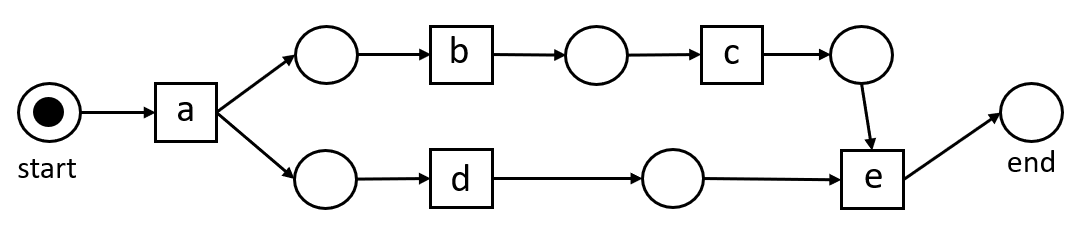
\includegraphics[width=0.8 \columnwidth]{figures/model1.png}
	\caption{The model of the process to which the case from Table \ref{table: table1} belongs. }
	\label{fig: model1}
	%width=1\columnwidth
\end{figure}
%
%
%
%


%extending the methods that measure how different or similar 

%\newpage
\begin{definition}[Petri Net]
A Petri Net is a tuple $N=(P,T,F)$ where $P$ is the set of places, $T$ the set of transitions, $P \cap T = \emptyset$ and $F \subseteq (P \times T) \cup (T \cup P)$.
A marking $M \in \mathcal{B}(P)$ is a multiset of places.
A petri net $N=(P,T,F)$ defines a directed bipartite graph where $P \cup T$ is the set of vertices and $F$ is the set of arcs.
\end{definition}

A marking describes the state of the petri net and it indicates how many \textit{tokens} are contained in each place.
For any place or transition $x \in P \cup T$, $\bullet x=\{x' \mid (x',x) \in F\}$ denotes the set of its input nodes, whereas $\bullet x=\{x' \mid (x,x') \in F\}$ denotes the set of its output nodes.
Note that the input and output nodes of places can only be transitions and vice-versa.
A transition is \textit{enabled} if there is at least one token in each of its input places.
An enabled transition can \textit{fire}, an action which removes one token from each input place and adds one token to each output place.
Given two markings $M$ and $M'$, we say that marking $M'$ is \textit{reachable} from $M$ if there exist transitions $\ t_1,...,t_n $ and markings $M_0,...,M_n$ such that $M_0=M$, $M_n=M'$, and for all $1 \leq i \leq n $: transition $t_i$ is enabled in $M_{i-1}$ and firing $t_i$ results in marking $M_i$.
In this case we also say that $M'$ is reachable from $M$ through the firing sequence $\langle t_1,...,t_n \rangle$.

\begin{definition}[Labeled Petri Net]
A labeled Petri Net $N=(P,T,F,\ell)$ is a Petri Net $(P,T,F)$ with a labeling function $\ell: ~ T \not \to \mathcal{U}_A$ which maps transitions to activity labels.
Given two markings $M$ and $M'$, we say $M'$ is reachable from $M$ through some activity sequence $\sigma_A$ if and only if there is a firing sequence $\sigma_T$ such that $M'$ is reachable from $M$ through $\sigma_T$ and $\ell(\sigma_T)=\sigma_A$.
\end{definition}


\begin{definition}[System Net]
A System Net is a triplet $SN=(N,M_{init},M_{final})$ where $N=(P,T,F,\ell)$ is a labeled Petri net, $M_{init} \in \mathcal{B}(P)$ is the initial marking, and $M_{final} \in \mathcal{B}(P)$ is the final marking.
Set $\phi(SN)$ contains all activity sequences through which $M_{final}$  is reachable from $M_{init}$.
\end{definition}

In Process Mining, we usually refer to any system net $(N,M_{init},M_{final})$ as a petri net with initial marking $M_{init}$ and final marking $M_{final}$.
We also call $\phi(SN)$ the set of \textit{replayable traces}.
Many process discovery algorithms applied on event data yield models in the form of petri nets.
The quality of those models depends on their simplicity, to what degree the replayable traces replicate exactly the traces from the log (\textit{fitness} and \textit{precision}) and so on.

\begin{definition}[Behavior Net \cite{conformance}] \label{def: bn}
Let $E \subseteq \mathcal{E}$ be the corresponding event set of some uncertain process instance, and let $bg(E)=(V,Arcs)$ be its behavior graph.
A behavior net $bn: \mathcal{P}(\mathcal{E}) \to \mathcal{U}_{SN}$ where $\mathcal{U}_{SN}$ denotes the universe of system nets is a system net $bn(E)=(P,T,F,\ell,M_{init},M_{final})$ such that:\\
-$P= Arcs \cup \\ 
\{(\textsc{start,v}) \mid \nexists_{v'\in V} s.t. (v',v) \in Arcs\} \cup  \\
\{(\textsc{v,\textsc{end}}) \mid \nexists_{v'\in V} s.t. (v,v') \in Arcs\}$\\
-$T=\{(v,a) \mid v \in V \wedge a \in \pi_a^{set}(v)\} \cup 
\{(v,\tau) \mid v \in V \wedge (\pi_o(v) = ? \vee \pi_o(v)=f_O \wedge f_O(?)>0 \}$\\
-$F= \{((\textsc{start},v_1),(v_2,a)) \in Arcs \times T \mid v_1 = v_2\} \cup \\
\{((v_1,a),(v_2,w)) \in T \times Arcs \mid v_1=v_2\} \cup \\
\{((w,v_1),(v_2,a)) \in Arcs \times T \mid v_1=v_2\} \cup \\
\{((v_1,a),(v_2,\textsc{end})) \in T \times Arcs \mid v_1 = v_2\} $\\
-$\ell=\{((v,a),a) \mid (v,a) \in T \wedge a \neq \tau\}$\\
-$M_{init} = [(\textsc{start},v) \mid v \in V]$\\
-$M_{final} = [(v,\textsc{end}) \mid v \in V]$.
\end{definition}


Similar to the behavior graph, the behavior net is a model that incorporates the uncertaity of a process instance.
As explained in \cite{conformance}, it is important to note that events whose timestamps overlap appear in an AND construct.
By definition of the behavior net, events which have a common predecessor in the behavior graph appear in an AND-split in the behavior net, whereas events that have a common sucessor in the behavior graph appear in an AND-join.
On the other hand, for events that have many possible activities, there is a transition for each of those activities in the behavior net and those transitions appear in and XOR-construct.
This indicates that every firing sequence starting in $M_{init}$ and ending in $M_{final}$ contains only one of those activities of the underlying event.
Similarly, whenever some event $e$ is indeterminate, there is also an explicit choice between a \textit{visible} transition, that is, a transition signaling the execution of a possible activity for $e$, and a \textit{silent} transition, which indicates skipping event $e$ by firing transition $(e,\tau)$.
It is shown in \cite{conformance} that the behavior net of an uncertain event set $E$ can replay all and only the activity trace realizations of $E$, that is: $\phi(bn(E)) = \mathcal{R}_a(E)$. 

The corresponding concept of the behavior net for certain process instances is the so-called \textit{event net}, which for a certain trace $\sigma$ of length $n$ contains $n$ visible transitions and $n+1$ places connected in a sequence.
The event net can only replay trace $\sigma$.
Note that the behavior graph of a certain trace would be a path of length $n-1$, containing $n$ vertices (one for each event) and $n-1$ arcs.\\

Next we introduce the concept of \textit{alignment} \cite{alignment}, which we later use to determine a conformance score between a trace and a given model.
\begin{definition}[Alignment]
Let $SN=(N,M_{init},M_{final})$ be a system net with $N=(P,T,F.\ell)$ 
and let $\sigma_L \in \mathcal{U}_A^*$ be some arbitrary trace.\\
An alignment between trace $\sigma_L$ and system net $SN$ is a pair $(\sigma_L^{\gg},\gamma_M^{\gg})$ with $\sigma_L^{\gg} \in (\mathcal{U}_a \cup \{\gg\})^*$ and $\gamma_M^{\gg} \in (T \cup \{\gg\})^*$, such that the following hold:\\
-$\sigma_L^{\gg} \downharpoonright_{\mathcal{U}_A} = \sigma_L$,\\
-$\gamma_M^{\gg} \downharpoonright_T = \gamma_M$ such that $M_{final}$ is reachable from $M_{init}$ through firing sequence $\gamma_M$,\\
-$|\sigma_L^{\gg}| = |\gamma_M^{\gg}| = n$ and for all $1 \leq i \leq n$ one of the following holds:
either $\sigma_L^{\gg}[i] = \ell(\gamma_M^{\gg}[i])$, or $\gamma_M^{\gg}[i] = \gg ~ \vee ~ \sigma_L^{\gg}[i] = \gg $.
\end{definition}
%
%
%
%
%\newpage
\begin{figure}[h!]
	\centering
	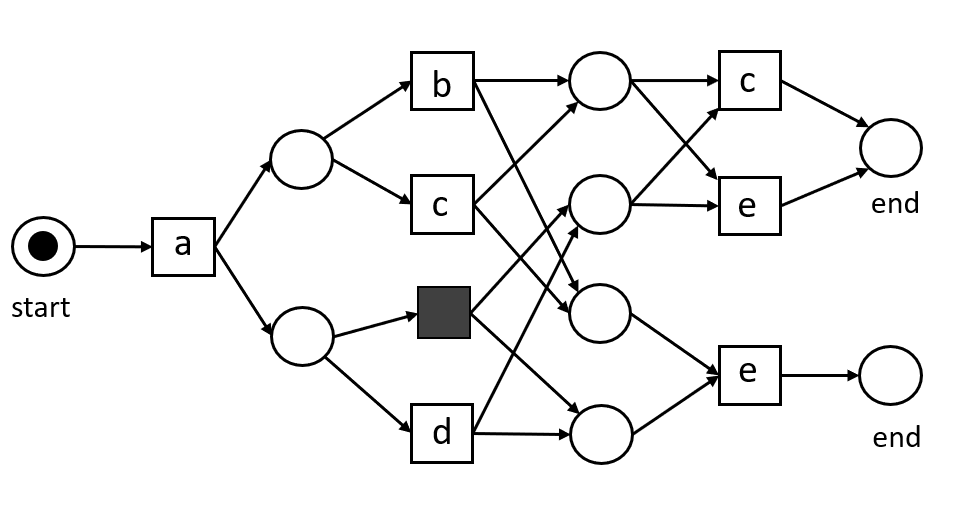
\includegraphics[width=0.8 \columnwidth]{figures/bn1.png}
	\caption{The behavior net corresponding to the event set from Table \ref{table: table1}. It can be constructed from the behavior graph shown in Figure \ref{fig: bg1}.}
	\label{fig: bn1}
	%width=1\columnwidth
\end{figure}
%
%
%
%
%
An alignment is used in conformance checking and describes a correspondence between a trace $\sigma_L$ from some log $L$ and a process model $M$, where each position in the alignment indicates a \textit{move}.
All the matching positions between the two sequences $\sigma_L^{\gg}$ and $\sigma_L^{\gg}$ as defined above indicate the similarities between trace $\sigma_L$ from the log and trace $\ell(\gamma_M)$ which is replayable in the model.
These moves are called the \textit{synchronous} moves.
If in a particular position sequence $\sigma_L^{\gg}$ contains symbol $\gg$, whereas $\gamma_M^{\gg}$ does not, this indicates a \textit{move only in the model}, implying that a particular behavior in the model is not replicated in the trace.
Similarly, if in a particular position sequence $\gamma_M^{\gg}$ contains symbol $\gg$, whereas $\sigma_L^{\gg}$ does not, this indicates a \textit{move only in the log}, implying that a particular behavior in the trace is not replicated in the model.
The \textit{cost} of an alignment depends on the number non-synchronous moves.
Usually, we assign cost 1 to \textit{only log moves} and \textit{only model moves}, and cost 0 otherwise.
While there might be more than one alignment between a trace and a model, the conformance score is determined by the cost of the optimal alignment between those two, that is, the alignment with minimal cost.
Such alignment describes how well the trace can be fitted in the model.
An alignment of cost 0 indicates that the trace is conforming to the model.
Not only do alignments provide a value quantifying conformance, but they also provide diagnostics by explicitly showing where a trace and a model deviate.
%
%
\begin{figure}[htp]
  \centering
 {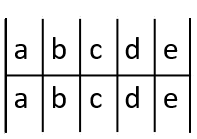
\includegraphics[width=30mm]{figures/align1.png}\label{align1}
	\subcaption{Optimal alignment between trace $\langle a,b,c,d,e \rangle$ and model from Fig. \ref{fig: model1} with cost 0.}
 	}
  %\hspace{2cm}
  {\label{align2}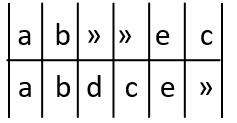
\includegraphics[width=36mm]{figures/align2.png}
	\subcaption{Optimal alignment between trace $\langle a,b,e,c \rangle$ and model from Fig. \ref{fig: model1} with cost 3.}
	}
	\label{fig: two alignments}
	\caption{Optimal alignments for two trace realizations of process instance from Table \ref{table: table1}.
	The projections of the first rows onto activity labels yield the two possible trace realizations, whereas the projections of the second rows onto activities yield the corresponding most similar traces from the model shown in Figure \ref{fig: model1}.}
\end{figure}
%
In this work, we also use the cost of optimal alignments as a measure for the conformance scores of possible trace realizations of uncertain process instances.
%
%
%
%
%
%
%

\chapter{Trace Realizations of Uncertain Process Instances} \label{chap:realizations}
In the remainder of this work, the starting point will be the set of events belonging to a particular uncertain process instance.
From now on, we assume we are given an uncertain log $L \subseteq \mathcal{E}$, where the case ID attribute of every event is always a unique value.
For every case $c \in \mathcal{U}_C^L$ and its corresponding event set $E_c$, we aim to estimate the probability of each possible activity trace corresponding to it.
For ease of notation, we omit the subscript $c$ when the case is clear from the context.

\section{Splitting Uncertain Traces}
We now show a naive method to compute the topological sortings of a directed acyclic graph through the \textsc{TopologicalSortings} algorithm (Algorithm \ref{alg:topo sortings}). 
Note that when the input graph is the follows graph of some event set $E$, according to Theorem \ref{theorem: topological sortings}, the topological sortings are equivalent to the correct evaluation orders on $(E,\prec_{\mathcal{E}})$.

\begin{algorithm}[h!]
	\caption{\textsc{TopologicalSortings($G$)}}
	\label{alg:topo sortings}
	\SetKwInOut{Input}{Input~}
	\SetKwInOut{Output}{Output~}
	\Input{~A directed graph $G=(V,A)$.}
	\Output{~Set $\mathcal{O}$ of topological sortings of $G$.}
	
	$\mathcal{S} \gets \mathcal{S}_V$ \tcp*{Set of all permutations over set $V$} \label{2: 1}
	
	\If{$|A| = 0$}{ \label{2: 2}
		\Return $\mathcal{S}$ \tcp*{All permutations are valid if $G$ has no arcs} \label{2: 3}} 
		
	$\mathcal{O} \gets \{ ~ \}$	\tcp*{Initialize set of valid permutations}
	
	\For{$s \in \mathcal{S}$}{ \label{2: 5}
		$previous \gets \{ ~ \}$ \tcp*{Events from $previous$ shouldn't appear \\ \label{2: 6}
		 later in $s$}
		$i \gets 1$
		
		\While{$i \leq |V|$}{ \label{2: 8}
			$current = s[i]$\\  \label{2: 9}
			\If{$i = |V|$}{ \label{2: 10}
				\If{$current \not \in previous$}{
					$\mathcal{O} \gets \mathcal{O} \cup {s}$ \label{2: 12}
					}
				}
			\Else{
				$incoming \gets \delta^{-}(s[i])$ \\ 
				\If{$(i=1 \wedge |incoming|>0) \vee current \in previous $ \label{2: 15} } 
				{
					\textbf{break} \tcp*{$s$ invalid, continue with next permutation} \label{2: 16}
					}
				$previous \gets previous \cup incoming$ \label{2: 17}	
				}
			}
		}
	\Return $\mathcal{O}$
	

\end{algorithm}

The algorithm goes through all permutations over the vertex set (line \ref{2: 5}) and adds the valid ones (the topological sortings) to set $\mathcal{O}$.
For a directed graph $G=(V,A)$ where $A$ is the set of arcs, for a particular vertex $v \in V$: 
$\delta^-(v)=\{u \in V \mid (u,v) \in A\}$ is the set of incoming neighbours of vertex $v$.
Note that if the current permutation is indeed a valid one, when encountering any vertex $v$ on position $i$, all vertices from $\delta^-(v)$ should have appeared previously in the permutation.
Otherwise, the permutation is not a topological sorting (Def. \ref{def: topological sorting} and Lemma \ref{lemma: edge path}).
For this reason, the set $previous$ is created for each permutation (line \ref{2: 6}) to contain all the vertices that should not appear later in the permutation.
We go through all vertices in their order of appearance in each permutation (lines \ref{2: 8}-\ref{2: 9}), and add their incoming neighbors to set $previous$ in line \ref{2: 17}.
If we later encounter some vertex from $previous$ in the current permutation, we discard the permutation as invalid and break (lines \ref{2: 15}-\ref{2: 16}).
Another reason to discard a permutation as invalid is if the current vertex is the first one in the current permutation, and it already has incoming neighbors, meaning vertices which should not appear after it (lines \ref{2: 15}-\ref{2: 16}).
We add the current permutation to the set of topological sortings in lines \ref{2: 10}-\ref{2: 12} if we make it to its last element without discarding it.

Note that it is the set of arcs in the input graph that poses constraints for the order of appearance of the vertices. 
If there are no arcs, then every permutation of the vertex set is valid (lines \ref{2: 2}-\ref{2: 3}). 

Computing $\mathcal{O}_G$ requires going through all permutations in $\mathcal{S}_V$ (a total number of $|V|!$ ) in order to obtain the ones which are a topological sorting.
When $V$ corresponds to a rather big event set, this might be problematic.
However, there might be many traces where despite uncertainty in timestamps, one can still partition the set of events of a case into smaller subsets which certainly happened sequentially. 
Think for example of processes with rather long traces where overlapping timestamps appear only in local parts of the process.
When the event set is timely partitioned, the task of computing $\mathcal{O}_G$ is reduced to computing the topological sortings (and this way, the correct evaluation orders) on the smaller subsets.
Depending on how well the uncertain trace can be fragmentized, this can help making the computation much more efficient.
Next, we explain how to obtain these subsets.
\pagebreak
%
%
% 
\begin{definition}[Comparability Graph]\label{def: comparability graph}
Let $E$ be the event set belonging to a process instance from some uncertain event log $L$.
The \emph{comparability graph} $\mathcal{C}omp(E)=(V_{\mathcal{C}omp},E_{\mathcal{C}omp})$ of event set $E$ is constructed as follows:
$V_{\mathcal{C}omp} = E$ and
$E_{\mathcal{C}omp} = \{ \{u,v\} \mid u \prec_{\mathcal{E}} v \vee v \prec_{\mathcal{E}} u\}$.
\end{definition}

\begin{proposition} \label{prop: comp = undirected}
Given an event set $E$, the comparability graph $\mathcal{C}omp(E)=(V_{\mathcal{C}omp},E_{\mathcal{C}omp})$ is the undirected variant of the follows graph $\mathcal{F}(E)=(V_{\mathcal{F}},E_{\mathcal{F}})$.
\end{proposition}

\begin{proof}
Let $\mathcal{F}(E)^U=(V_{\mathcal{F}}^U,E_{\mathcal{F}}^U)$ be the undirected variant of $\mathcal{F}(E)$ as defined in \ref{def: undirected variant}.
It holds that $V_{\mathcal{C}omp} = E = V_{\mathcal{F}} = V_{\mathcal{F}}^U$ by Def. \ref{def: comparability graph}, \ref{def: follows graph} and \ref{def: undirected variant} respectively.
Additionally, it holds that $\{u,v\} \in E_{\mathcal{C}omp} 
\overset{Def.\ref{def: comparability graph}}{\Longleftrightarrow} 
u \prec_{\mathcal{E}} v \vee v \prec_{\mathcal{E}} u 
\overset{Def. \ref{spo}}{\Longleftrightarrow}
(u \prec_{\mathcal{E}} v \vee v \prec_{\mathcal{E}} u) \wedge u \neq v
\overset{Def.\ref{def: follows graph}}{\Longleftrightarrow}
((u,v) \in E_{\mathcal{F}} \vee (v,u) \in E_{\mathcal{F}}) \wedge u \neq v
\overset{Def.\ref{def: undirected variant}}{\Longleftrightarrow}
\{u,v\} \in E_{\mathcal{F}}^U$.
%\qed
\end{proof}
 
The comparability graph is undirected and it contains an edge between a pair of events $e,e' \in E$ if and only if their time intervals are comparable, that is, there is no overlapping of their possible timestamps.
By ignoring the direction of the arcs in the follows graph, the comparability graph focuses on whether event pairs can be ordered in time, instead of indicating which one is the predecessor or the successor.


\begin{definition}[Interval Graph]\label{def: interval graph}
Let $E$ be the event set belonging to a process instance from some uncertain event log $L$.
The \emph{interval graph} of event set $E$ is the graph $\mathcal{I}(E)=(V_{\mathcal{I}},E_{\mathcal{I}})$ where
$V_{\mathcal{I}} = E$ and 
$E_{\mathcal{I}} = \{ \{u,v\} \mid t_{min}(u) \leq t_{max}(v) \wedge t_{min}(v) \leq t_{max}(u)\}$.
\end{definition}
Note that in the interval graph, two events are connected by an edge if and only if they have overlapping timestamps.
%\begin{proposition}
%Let $\mathcal{I}(E)=(V_{\mathcal{I}},E_{\mathcal{I}})$ be the interval graph of some event set $E$.
%Given $u,v \in V_{\mathcal{I}}$, it holds that $\{u,v\} \in E_{\mathcal{I}}$ if and only if $u$ and $v$ are not comparable w.r.t. $\prec_{\mathcal{E}}$.
%\end{proposition}

%\begin{proof}
%Let $u$ and $v$ be two events which have overlapping timestamps, that is, they are not comparable w.r.t $\prec_{\mathcal{E}}$.
%It holds that $u,v \in E$ not comparable w.r.t. $\prec_{\mathcal{E}} \Leftrightarrow
%u \not \prec_{\mathcal{E}} v \wedge v \not \prec_{\mathcal{E}} u
%\Leftrightarrow
%t_{max}(u) \not < t_{min}(v) \wedge t_{max}(v) \not < t_{min}(u)
%\Leftrightarrow
%t_{max}(u) \geq t_{min}(v) \wedge t_{max}(v) \geq t_{min}(u)
%\Leftrightarrow
%\{u,v\} \in E_{\mathcal{I}}$.
%\qed
%\end{proof}
%


\begin{proposition}\label{prop: interval = complement}
Given an event set $E$, the interval graph $\mathcal{I}(E)=(V_{\mathcal{I}},E_{\mathcal{I}})$ is the complement of the comparability graph $\mathcal{C}omp(E)=(V_{\mathcal{C}omp},E_{\mathcal{C}omp})$.
\end{proposition}

\begin{proof}
Let $\overline{\mathcal{C}}=\overline{\mathcal{C}omp(E)}=(V_{\overline{\mathcal{C}}}, E_{\overline{\mathcal{C}}})$ be the complement of the comparability graph $\mathcal{C}omp(E)=(V_{\mathcal{C}omp},E_{\mathcal{C}omp})$ of event set $E$.
It holds that $V_{\mathcal{I}}=E=V_{\mathcal{C}omp}=V_{\overline{\mathcal{C}}}$ by Def. \ref{def: interval graph}, \ref{def: comparability graph} and \ref{def: complement graph} respectively.
Additionally, it holds that 
$ \{u,v\} \in E_{\mathcal{I}}
\overset{Def. \ref{def: interval graph}}{\Longleftrightarrow}
t_{min}(u) \leq t_{max}(v) \wedge t_{min}(v) \leq t_{max}(u)
\overset{}{\Longleftrightarrow}
\neg \big( t_{min}(u) > t_{max}(v) \vee t_{min}(v) > t_{max}(u) \big)
\overset{Def. \ref{spo}}{\Longleftrightarrow}
\neg \big( v \prec_{\mathcal{E}} u \vee u \prec_{\mathcal{E}} v \big)
\overset{Def. \ref{def: comparability graph}}{\Longleftrightarrow}
\{u,v\} \not \in E_{\mathcal{C}omp}
\overset{Def. \ref{def: complement graph}}{\Longleftrightarrow}
\{u,v\} \in E_{\overline{\mathcal{C}}}
$.
%\qed
\end{proof}


\begin{theorem}\label{theorem: partitioning}
Let $\mathcal{I}(E)=(V_{\mathcal{I}},E_{\mathcal{I}})$ be the interval graph of some event set $E$.
The connected components of $\mathcal{I}(E)$ partition set $E$ into subsets of minimal size such that any two events from different subsets can be ordered in time.
\end{theorem}


\begin{proof}
\leavevmode \\ 
(1) \textit{Any two events from different components of the interval graph appear in the $\prec_{\mathcal{E}}$ relation.}\\
Suppose that $C_1, C_2 \subseteq V$ are two connected components of $\mathcal{I}(G)$ and let $e_1 \in C_1, e_2 \in C_2$ be two arbitrary vertices (representing events $e_1$ and $e_2$) from these components.
We know that $\{e_1,e_2\} \not \in E_{\mathcal{I}}$.
Since the interval graph is the complement graph of $\mathcal{C}omp(E)$ (Prop. \ref{prop: interval = complement}), then $\{e_1,e_2\} \in E_{\mathcal{C}omp}$.
By definition of the comparability graph, either $e_1 \prec_{\mathcal{E}} e_2$ or $e_2 \prec_{\mathcal{E}} e_1$ must hold.\\ \\
(2) \textit{There is no finer partition on the event set that satisfies (1) than the one induced by the connected components of the interval graph.}\\
Let $\mathcal{I}(E)$ be the interval graph of $E$  and let $V= C_1 \cup ... \cup C_n$ be its partition into connected components for which (1) holds.
Assume there is some component $C$ from $\{C_1,...,C_n\}$ which can be further partitioned into two non-empty subsets $C=C' \cup C''$ so that claim (1) still holds.
Let $e' \in C', e'' \in C''$ be two arbitrary vertices from $C'$ and $C''$.
Since $e',e'' \in C$, it holds that $\{e',e''\} \in E_{\mathcal{I}}$. 
Since the interval graph is the complement of the comparability graph $\mathcal{C}omp(E)$, then $\{e',e''\} \not \in E_{\mathcal{C}omp}$.
This means that both $e' \not \prec_{\mathcal{E}} e''$ and $e'' \not \prec_{\mathcal{E}} e'$ hold.
This contradicts the assumption that $C'$ and $C''$ satisfy (1).
%\qed
\end{proof}

\begin{proposition}\label{prop: clique}
Let $\mathcal{I}(E)=(V_{\mathcal{I}},E_{\mathcal{I}})$ be the integral graph of some event set $E$ and let $C \subseteq V_{\mathcal{I}}$ be some connected component of $\mathcal{I}(E)$.
If $C$ is a clique, then every permutation $s \in \mathcal{S}_C$ is a correct evaluation order on $(C,\prec_{\mathcal{E}})$.
\end{proposition}

\begin{proof} 
Let $C=\{e_1,...,e_{|C|}\}$ be a connected component of $\mathcal{I}(E)$ which is a clique.
Then, $\forall i,j \in \{1,...,|C|\}$ s.t. $i\neq j$, the pair $e_i, e_j$ is connected through an edge in $\mathcal{I}(E)$.
Since the interval graph $\mathcal{I}(E)$ is the complement of the comparability graph $\mathcal{C}omp(E)$, it holds from Prop. \ref{prop: interval = complement} that for every such pair of vertices, there is no edge between them in $\mathcal{C}omp(E)$.
This implies that $\forall i,j \in \{1,...,|C|\}$ s.t. $i \neq j$, neither $e_i \prec_{\mathcal{E}} e_j$ nor $e_j \prec_{\mathcal{E}} e_i$ hold.
This way, for every permutation $s \in \mathcal{S}_C$, the condition
$\forall ~ 1 \leq i < j \leq |s|: ~ s[j] \not \prec_{\mathcal{E}} s[i]$ is always satisfied.
Therefore, every $s \in \mathcal{S}_C$ is a correct evaluation order on $(C, \prec_{\mathcal{E}})$. 
%\qed 
\end{proof}

The claim in Proposition \ref{prop: clique} is not surprising, since it is equivalent to saying that all permutations of an event set are valid if their corresponding follows graph has no arcs.


%$(\Leftarrow)$
%Let $C=\{e^C_1,...,e^C_{|C|}\}$ be a set of events for which every permutation $s \in \mathcal{S}_C$ is a correct evaluation order on $(C,\prec_{\mathcal{E}})$.
%Then from Definition \ref{eval} follows that there are no $i,j \in \{1,...,|C|\}, i\neq j$ such that $s[i] \prec_{\mathcal{E}} s[j]$.
%Otherwise, every permutation where $s[j]$ appears before $s[i]$ would not be a correct evaluation order on $(C,\prec_{\mathcal{E}})$.
%This is equivalent to the claim: For every pair $i,j \in \{1,...,|C|\}, i\neq j$ it holds that neither $e^C_i \prec_{\mathcal{E}} e^C_j$ nor $e^C_j \prec_{\mathcal{E}} e^C_i$ hold.
%From Definition \ref{comp graph} of the comparability graph follows that $(e^C_i,e^C_j) \not \in E_{\mathcal{C}}$


\begin{proposition}\label{prop: component size}
Let $E$ be some event set and let $\mathcal{F}(E)$ be its corresponding follows graph.
If $\mathcal{F}(E)$ has more than one connected component, then only one of these components has size greater than 1.
\end{proposition}


\begin{proof}
%Let $E$ be some event set and let $\mathcal{F}(E)$ be its corresponding follows graph.
Assume there are two connected components $C', C''$ in $\mathcal{F}(E)$ which both have size greater than 1.
Note that we can always find two events from each component: $e_1, e_2 \in C'$ and $e_3, e_4 \in C''$,
such that both arcs $(e_1,e_2)$ and $(e_3,e_4)$ exist in $\mathcal{F}(E)$.
From the definition of the follows graph, we know that the following hold: 
$t_{max}(e_1) < t_{min}(e_2)$ and $t_{max}(e_3) < t_{min}(e_4)$.
Also, since the pairs lie in different connected components of $\mathcal{F}(E)$, there is no arc $(u,v)$ in $\mathcal{F}(E)$ such that $u \in C'$ and $v \in C''$ or vice-versa.
Since there is no arc between $e_3$ and $e_2$, it holds that $t_{min}(e_2) \leq t_{max}(e_3)$ (because $t_{max}(e_3) \not < t_{min}(e_2))$. 
From this follows:
$t_{max}(e_1) < t_{min}(e_2) \leq t_{max}(e_3) < t_{min}(e_4)$.
But this implies that $t_{max}(e_1) < t_{min}(e_4)$ so there must be an arc between $e_1$ and $e_4$.
%\qed
\end{proof}
%\textcolor{red}{Note:}
Equivalently, the claim in Proposition \ref{prop: component size} can be proved by showing that every interval graph is chordal (it has no cycle of length $\geq$ 4).
%\begin{proposition}
%Let $E$ be some event set and let $\mathcal{F}(E)$ and $\mathcal{I}(E)$ be its corresponding follows and interval graph respectively.
%Let $C_1,...,C_n$ be the connected components of the interval graph $\mathcal{I}(E)$.
%For all $i=1,..,n$ it holds that $\mathcal{F}(E)[C_i]$ has at most one connected component of size greater than 1.
%\end{proposition}
%\begin{proof}
%Follows directly from Proposition \ref{comp size}.
%\end{proof}
Propositions \ref{prop: clique} and \ref{prop: component size} contain two claims which we will exploit when constructing the set of correct evaluation orders in the next section.
Proposition \ref{prop: clique} says that if a connected component of the interval graph is a clique, then all permutations of its vertices induce topological sortings and thus also correct evaluation orders.
If the subgraph is not a clique, then we have to look at the corresponding follows graph in order to obtain the topological sortings.
According to Proposition \ref{prop: component size}, in this subgraph there is at most one connected component with more than one node and thus a non-trivial set of topological sortings. 
From here on, one could repeat the same reasoning for the subgraphs of the follows graph: using their interval graphs to split  them and then repeat the procedure until we arrive at trivial components of size one.
One would then have to merge their corresponding permutations step by step into full sequences.
The way the smaller subsequences should be merged depends on whether the graph components they were part of during the split belonged to the follows graph or the interval graph.
This is the idea behind the method that we introduce in the next section.
%
%
%
%
\section{Computing Event Trace Realizations: A New Approach}
In this section, we introduce an algorithm (Algorithm \ref{alg:valid permutations}) which computes the set of event trace realizations of a given event set $E$ in a non-naive way by exploiting the claims from Theorem \ref{theorem: partitioning}, Propositions \ref{prop: clique} and \ref{prop: component size}.
It relies on the following two arguments:
\begin{itemize}
\item Let $G$ be some directed acyclic graph with connected components $C_1,..,C_n$ where w.l.o.g. $C_1$ is the (only) big component.
Let $\mathcal{S}_1$ be the set of topological sortings of $G[C_1]$.
Then, any permutation $s \in \mathcal{S}_{V(G)}$ is a topological sorting in $G$ if and only if there exists $s_1 \in \mathcal{S}_1$ such that the elements of $s_1$ appear in $s$ in the same order: $s \downharpoonright_{C_1} = s_1$ ($s$ projected onto set $C_1$).
%\textcolor{red}{This is a bit complicated in the algorithm, corresponding part in the swappingAlg must be changed. It has to be done because it is still better than going through all permutations. Otherwise one could remove the whole recursive method and just do naive topological sorting on the first-level connected components of the interval graph}.
\item Given some follows graph $\mathcal{F}$ and its corresponding interval graph $\mathcal{I}$ which has $m$ connected components, one can timely order the components into $\langle C_1,...,C_m \rangle$ such that $\forall ~ 1 \leq i<j \leq m: ~ e_i \prec_{\mathcal{E}} e_j$ for every pair $e_i \in C_i$ and $e_j \in C_j$.
This follows from Theorem \ref{theorem: partitioning}.
Moreover, the topological sortings of $\mathcal{F}$ are the sequences $\langle s^1,...,s^m \rangle$ such that for all $i \in \{1,...,m\}$: $s^i$ is a topological sorting of $\mathcal{F}[C_i]$.
\end{itemize}
These two points constitute the idea behind our new method for computing the event trace realizations.
%On one hand, we use Algorithm \ref{alg: FollowsGraph Splitting} to handle each connected component of the follows graph separately.
%The valid permutations of these components are merged together using Algorithm \ref{alg:combine with}.
%The name \textsc{CombineWithSwapping} of Algorithm \ref{alg:combine with} indicates that any order of the sequences emerging from different follows graph components is valid. 
%The \textsc{Interweave} method used in Algorithm \ref{alg:combine with} exploits the knowledge that only one component might be of size greater than 1 to compute the merges more efficiently.
%For each component of the interval graph on the other hand, Algorithm \ref{alg: IntervalGraph Splitting} handles the connected components of the interval graph and detects their ordering.
%Their valid sequences are then merged together according to this order using Algorithm \ref{alg:combine without}.
%The name \textsc{CombineWithoutSwapping} of Algorithm \ref{alg:combine without} indicates that the components' order in the interval graph is fixed and no swapping takes place.
%
%Algorithms \ref{alg: FollowsGraph Splitting} and \ref{alg: IntervalGraph Splitting} call each-other interchangeably to efficiently make use of the graph structure to prune all invalid permutations of the vertices.
%The recursion breaks when the graph for which the valid permutations have to be computed has a single node.
%The recursion might be stopped earlier if in the \textsc{IntervalGraphSplitting} method it is noticed that the interval graph of a given connected follows graph still has no more than one single component.
%Here the algorithm relies again on the naive way using the \textsc{TopologicalSortings} method to obtain the valid permutations on that particular subgraph.
%In the end, the output of Algorithm \ref{alg:valid permutations} is a set containing all valid permutations on the input event set.
%
%
%
%
%
%
%
%
%
%
%
%
\begin{algorithm}[h!]
	\caption{\textsc{CombineWithSwapping}($\{P_1,...,P_k \}$)}
	\label{alg:combine with}
	\SetKwInOut{Input}{Input~}
	\SetKwInOut{Output}{Output~}
	\Input{~A set of sets $P_i$ each containing sequences.}
	\Output{~Set of (full sequences) where each is a combination of sequences from the sets $P_i$ in any possible order.}	
	
	\If{$k=1$}{
		\Return $P$ \tcp*{Nothing to merge when there is only one set}
		} 
	\If{$\forall 1 \leq i \leq k: ~ |P_i[1]| = 1$}{
		\Return $S_{\{s_1,...,s_k\}}$ \tcp*{Here, all $P_i$-s are singleton sets, \\ so all permutations are valid.}}
		
		
	$FullSequences \gets \{ ~ \}$	
	
	$orderedSets \gets list(P_1,...,P_k)$ \tcp*{create some arbitrary ordering}
	
	$b \gets BigComponent(P_1,...,P_k)$ \tcp*{identifying the index of the \\ (single) set with non-trivial sequences}
	
	$swappings = \mathcal{S}_{\{1,...,k\} \setminus \{b\}}$ \tcp*{all possible swappings of singleton sets}
	
	$singletonPermutations \gets \{ ~ \}$
	
	\For{$swap \in swappings$}{
		$combinedSingletons \gets \bigotimes_{j=swap[1]}^{swap[|swap|]} P_j $	
		
		\For{$s \in combinedSingletons$}{
			$singletonPermutations \gets singletonPermutations \cup \{\widehat{s}\}$ \tcp*{All \\ permutations without the big component}
			}	
		}
	$FullSequences \gets \{~\}$ \\
	
	%\textcolor{blue}{	
	\For{$s_b \in P_b$}{ \label{3: 15}
		\For{$s \in singletonPermutations$}{
			$interweavings \gets $ \textsc{Interweave}($s_b,s$) \\
			$FullSequences \gets FullSequences \cup interweavings$
			} \label{3: 18}
		}
	%}
	\Return $FullSequences$
\end{algorithm}
%\caption{Given sets $P_1,...,P_k$ where each one contains sequences, \emph{combining} them means obtaining the (flattened) full sequences from their cartesian product, while \emph{swapping} means that all orderings of sets in the cartesian product are possible.}
%
%
%
%
%
%
%
%
%
%
%
%
\begin{algorithm}[h!]
	\caption{\textsc{Interweave}($s_b,s$)}
	\label{alg:place}
	\SetKwInOut{Input}{Input~}
	\SetKwInOut{Output}{Output~}
	\Input{~Two sequences $s_b$ and $s$ where $s_b$ comes from the big component and $s$ is a permutation of singleton sequences.}
	\Output{~A list of full sequences interweaving elements from $s_b$ and $s$ without changing the ordering.}	

	\If{$s_b=\langle ~ \rangle$ \tcp*{stop when all elements from $s_b$ were picked}}{
		\Return ${s}$}
		
	$interweavings \gets \{ ~ \} $ \\
	$event \gets s_b[1]$ \tcp*{Start with first element of $s_b$}
	
	\For{$pos \in \{0,...,|s|\}$}{
		$s_{new} \gets s$ \tcp*{create a copy of sequence $s$}
		$s_{new}.insert(pos,event)$ \tcp*{Insert event to $s$ at position $pos$} 
		$interweavings \gets interweavings \cup \{
		 \textsc{Interweave}(s_b[2:],s_{new}, pos+1) \} $  %\tcp*{insert the rest of $s_b$ }
		}
	\Return $interweavings$
		
\end{algorithm}
%
%
%
%
%
%
%
%
%
%
%
%
\begin{algorithm}[h!]
	\caption{\textsc{CombineWithoutSwapping}($\langle P_1,...,P_k \rangle$)}
	\label{alg:combine without}
	\SetKwInOut{Input}{Input~}
	\SetKwInOut{Output}{Output~}
	\Input{~A list of sets $P_i$, each containing sequences.}
	\Output{~Set of (full) sequences where each comes from the cartesian product of the $P_i$-s.}
	
	\If{$k=1$}{
		\Return $P$ \tcp*{Nothing to merge when there is only one set}
		}
		
	$FullSequences \gets \{ ~ \}$	
	
	$combinedSequences \gets \bigotimes_{i=1}^k P_i$ \tcp*{cartesian product of sets} \label{5: 4}
	
	\For{$s \in combinedSequences$}{
		$FullSequences \gets FullSequences \cup \{\widehat{s}\}$ 
		\tcp*{flatten list $s$} \label{5: 6}
		}		
	\Return $FullSequences$
\end{algorithm}
%
%
%
%
%
%
%
%
%
%
%
%
\begin{algorithm}[h!]
	\caption{\textsc{FollowsGraphSplitting($\mathcal{F},\mathcal{I},V$)}}
	\label{alg: FollowsGraph Splitting}
	\SetKwInOut{Input}{Input~}
	\SetKwInOut{Output}{Output~}
	\Input{~A directed acyclic graph $\mathcal{F}$ and its corresponding interval graph $\mathcal{I}$, $V$ a subset of their vertex set.}
	\Output{~Set $\mathcal{O}$ of topological sortings of $\mathcal{F}[V]$.}
		
	
	\If{$V=\{v\}$}{ \label{6: 1}
		\Return $\{ \{ \langle v \rangle \} \}$ \tcp*{If $V$ has only one vertex, return \\ single set with trivial topo. sorting}
		}	\label{6: 2}
	$G \gets \mathcal{F}[V]$\\ \label{6: 3}
	$components \gets CC(G)$ \tcp*{Compute connected components of $G$} \label{6: 4}
	
	%$n_c \gets |components|$
	
	$P_{sets} \gets \{ ~ \}$
	
	\For{$C \in components$}{ \label{6: 6}
		$P_i \gets \textsc{IntervalGraphSplitting}(\mathcal{F},\mathcal{I},C)$		\label{6: 7}
		
		$P_{sets} \gets P_{sets} \cup \{\{P_i\}\}$
		}	
	$\mathcal{O} \gets \textsc{CombineWithSwapping}(P_{sets})$ \label{6: 9}
	
	
	\Return $\mathcal{O}$
\end{algorithm}
%
%
%
%
%
%
%
%
%
%
\begin{algorithm}[h!]
	\caption{\textsc{IntervalGraphSplitting($\mathcal{F},\mathcal{I},V$)}}
	\label{alg: IntervalGraph Splitting}
	\SetKwInOut{Input}{Input~}
	\SetKwInOut{Output}{Output~}
	\Input{~A directed acyclic graph $\mathcal{F}$ and its corresponding interval graph $\mathcal{I}$, $V$ a subset of their vertex set.}
	\Output{~Set $\mathcal{O}$ of topological sortings of $\mathcal{F}[V]$.}
	
	
	\If{$V=\{ v\}$}{ \label{7: 1}
		\Return $\{\{ \langle v \rangle \}\}$ \tcp*{If $V$ has only one vertex, return \\ trivial topo. sorting} \label{7: 2}
		}
	
	$G \gets \mathcal{I}[V]$\\	\label{7: 3}
	$components \gets CC(G)$ \tcp*{Compute connected components of $G$} \label{7: 4}
	
	 \If{$|components| = 1$}{ \label{7: 5}
		$\mathcal{O} \gets \textsc{TopologicalSortings}(\mathcal{F}[V])$ \tcp*{If graph cannot be splitted \\ further, use naive method.} \label{7: 6}
		\Return $\mathcal{O}$	
	 	}
	 	
	$C_{list} \gets \langle ~ \rangle$ \label{7: 8}
	
	\For{$C \in components$}{
		$start \gets min\{t_{min}(e) \mid e \in C\}$
		}
		
		$C_{list} \gets C_{list} \oplus (start,C)$
	
	$\textsc{Sort}(C_{list})$ \tcp*{Sort components on their minimal timestamps} \label{7: 12}
	
	$P_{list} \gets \langle ~ \rangle$
	
	\For{$C \in C_{list}$}{ \label{7: 14}
	
		$P_i \gets\textsc{FollowsGraphSplitting}(\mathcal{F},\mathcal{I},C)$ \label{7: 15}
		
		$P_{list} \gets P_{list} \oplus P_i$		
		}
	
	$\mathcal{O} \gets \textsc{CombineWithoutSwapping}(P_{list})$ \label{7: 17}
	
	\Return $\mathcal{O}$
\end{algorithm}
%
%
%
%
%
%
%
%
%
%
\begin{algorithm}[h!]
	\caption{\textsc{ValidPermutations($E$)}}
	\label{alg:valid permutations}
	\SetKwInOut{Input}{Input~}
	\SetKwInOut{Output}{Output~}
	\Input{~An event set $E$.}
	\Output{~Set $\mathcal{R}_e(E)$ of correct evaluation orders on $(E,\prec_{\mathcal{E}})$.}

	$\mathcal{F} \gets \textsc{FollowsGraph}(E)$ \label{8: 1}
	
	$\mathcal{C}omp \gets \mathcal{F}^U$ \tcp*{Build undirected variant of $\mathcal{F}$.} \label{8: 2}
	
	$\mathcal{I} \gets \overline{\mathcal{C}omp}$ \tcp*{Build complement graph of $\mathcal{C}omp$.} \label{8: 3}
	
	$\mathcal{R}_e \gets \textsc{FollowsGraphSplitting}(\mathcal{F},\mathcal{I},V_{\mathcal{F}})$ \label{8: 4}
	
	\Return $\mathcal{R}_e$
\end{algorithm}
%
%
%
%
%
%\newpage

We first construct the follows and interval graph of the given event set in lines \ref{8: 1}-\ref{8: 3} of Algorithm \ref{alg:valid permutations}.
Then, the \textsc{FollowsGraphSplitting} method is called on the follows- and interval graph with the original vertex set in line \ref{8: 4}.
The \textsc{FollowsGraphSplitting} method in Algorithm \ref{alg: FollowsGraph Splitting} handles subgraphs of the follows graph induced by the input vertex set (line \ref{8: 3}).
If the graph has a single node, the trivial permutation is returned for that subgraph (lines \ref{6: 1}-\ref{6: 2}).
Otherwise, the connected components are detected (line \ref{6: 4}), and for each of those components the interval graph technique is used by calling the \textsc{IntervalGraphSplitting} method in Algorithm  \ref{alg: IntervalGraph Splitting} (lines \ref{6: 6}-\ref{6: 7}).
The valid partial permutations yielded by Algorithm \ref{alg: IntervalGraph Splitting} for each of those components are then merged back together using the \textsc{CombineWithSwapping} method (line \ref{6: 9}).
This indicates that valid permutations of different components originating from the follows graph can be combined together in any order, as long as the ordering within the component is preserved.
From Proposition \ref{prop: component size} we know that there is at most one component of size greater than 1.
Whenever that is the case, the \textsc{CombineWithSwapping} method in Algorithm \ref{alg:combine with} calls the \textsc{Interweave} function (lines \ref{3: 15}-\ref{3: 18}), which constructs all valid mergings of the singleton components with the big component.

As we mentioned, the \textsc{IntervalGraphSplitting} method in Algorithm \ref{alg: IntervalGraph Splitting} is applied on a connected component of the follows graph and handles the subgraph of the interval graph induced by the input vertex set. 
In the end, it yields the valid permutations on the input vertex set of that component.
To do this, it first checks whether the input is a single vertex in line \ref{7: 1}.
If that is the case, then the trivial permutation is returned in line \ref{7: 2}.
Otherwise, the subgraph of the interval graph induced by the input vertex set is computed in line \ref{7: 3}.
The set of connected components in the subgraph of the interval graph is computed (line \ref{7: 4}) and their order is detected (lines \ref{7: 8}-\ref{7: 12}).
Each of those components represents a smaller instance of the original input, that is, smaller vertex sets for which the valid orderings have to be computed according to the arcs connecting them in the original follows graph.
At this point, the next recursion round starts, where the \textsc{FollowsGraphSplitting} method is called on each component of the interval graph (lines \ref{7: 14}-\ref{7: 15}).
Since those components have a fixed ordering which was computed before, to merge them back together the \textsc{CombineWithoutSwapping} method from Algorithm \ref{alg:combine without} is used (line \ref{7: 17}).
As the name indicates, the partial permutations of the components originating from an interval graph subgraph are combined with a fixed order.
This is easily done by obtaining the cartesian product of the sets containing the valid sequences of each component (lines \ref{5: 4}-\ref{5: 6} of Algorithm \ref{alg:combine without}).
It could also happen that the interval graph corresponding to the follows graph induced by the input vertex set in the \textsc{IntervalGrapSplitting} method does not further split the vertex set into smaller sets.
Continuing the recursion with the \textsc{FollowsGraphSplitting} method here would lead to non-termination.
For this reason, in the \textsc{IntervalGraphSplitting} method in Algorithm \ref{alg: IntervalGraph Splitting}, we check whether the subgraph of the interval graph induced by the input vertex set has only one component (line \ref{7: 5}). 
Whenever that is the case, we fall back on the naive \textsc{TopologicalSortings} method of Algorithm \ref{alg:topo sortings} to obtain the set of valid sequences for that vertex subset (line \ref{7: 6}).
In the end, all valid subsequences are merged together to yield the full valid permutations.\\
Next, we see how the algorithm is applied on a running example. 
%
%
%
%
%

\newpage
Suppose an uncertain trace consists of the 8 uncertain events which are shown in Table \ref{table:8 events}.
We apply Algorithm \ref{alg:valid permutations} to this set of events in order to efficiently obtain the set of correct evaluation orders on this set.

\begin{table}[h!]
	\centering
	\caption{A set of 8 uncertain events corresponding to the process instance identified through case ID 1112.}
	\begin{tabular}{ccccc}
		\textbf{Case ID} & \textbf{Event ID}        & \textbf{Activity}                                                                                                     & \textbf{Timestamp}             & \multicolumn{1}{l}{\textbf{Event Type}} \\ \hline
		\multicolumn{1}{|c|}{1112} & \multicolumn{1}{|c|}{$e_1$} &
		\multicolumn{1}{c|}{a} & \multicolumn{1}{c|}{\begin{tabular}[c]{@{}c@{}} 02-12-2020\end{tabular}}                                                                                 & \multicolumn{1}{c|}{!}                    \\ \hline
		\multicolumn{1}{|c|}{1112} & \multicolumn{1}{|c|}{$e_2$} &
		\multicolumn{1}{c|}{b} & \multicolumn{1}{c|}{\begin{tabular}[c]{@{}c@{}}[01-12-2020, 03-12-2020]\end{tabular}}                                                                         &  \multicolumn{1}{c|}{!}                    \\ \hline
		\multicolumn{1}{|c|}{1112} & \multicolumn{1}{|c|}{$e_3$} &
		\multicolumn{1}{c|}{c}        & \multicolumn{1}{c|}{\begin{tabular}[c]{@{}c@{}}[04-12-2020, 05-12-2020]\end{tabular}}                                                                          &	\multicolumn{1}{c|}{!}                    \\ \hline
		\multicolumn{1}{|c|}{1112} & \multicolumn{1}{|c|}{$e_4$} &
		\multicolumn{1}{c|}{d} & \multicolumn{1}{c|}{\begin{tabular}[c]{@{}c@{}}[06-12-2020, 07-12-2020]\end{tabular}}                                                                         &  \multicolumn{1}{c|}{!}                    \\ \hline
		\multicolumn{1}{|c|}{1112} & \multicolumn{1}{|c|}{$e_5$} &
		\multicolumn{1}{c|}{e}        & \multicolumn{1}{c|}{\begin{tabular}[c]{@{}c@{}}09-12-2020 \end{tabular}}                                                                         &  \multicolumn{1}{c|}{!}                    \\ \hline
		\multicolumn{1}{|c|}{1112} & \multicolumn{1}{|c|}{$e_6$} &
		\multicolumn{1}{c|}{f} & \multicolumn{1}{c|}{\begin{tabular}[c]{@{}c@{}}[08-12-2020, 10-12-2020]\end{tabular}}                                                                         &  \multicolumn{1}{c|}{!}                    \\ \hline
		\multicolumn{1}{|c|}{1112} & \multicolumn{1}{|c|}{$e_7$} &
		\multicolumn{1}{c|}{g} & \multicolumn{1}{c|}{\begin{tabular}[c]{@{}c@{}}[04-12-2020, 10-12-2020]\end{tabular}}                                                                          &  \multicolumn{1}{c|}{!}                    \\ \hline
		\multicolumn{1}{|c|}{1112} & \multicolumn{1}{|c|}{$e_8$} &
		\multicolumn{1}{c|}{i}        & \multicolumn{1}{c|}{\begin{tabular}[c]{@{}c@{}}13-12-2020 \end{tabular}}                                                                         &  \multicolumn{1}{c|}{!}                    \\ \hline
		\end{tabular}
		\caption{A set of 8 uncertain events corresponding to the process instance identified with case ID 1112.}
		\label{table:8 events}
\end{table}
%
Fig. \ref{fig:follows graph} and \ref{fig:interval graph} show the initial follows graph and interval graph of the given event set.
%
%
%
%
%
%
%
%
%
%
\begin{figure}[h]
	\centering
	%\resizebox{\textwidth}{!}
	{
	\begin{tikzpicture}[->,>=stealth',shorten >=1pt,node distance=2.5cm,auto,main node/.style={circle,draw,align=center}]
	\node[main node]	(A)	at (0,2)			{$e_1$};
	\node[main node]	(B)	at (0,0)			{$e_2$};
	\node[main node]	(C)	at (2,2)			{$e_3$};
	\node[main node]	(D)	at (4,2)			{$e_4$};
	\node[main node]	(E)	at (6,3)       		{$e_5$};
	\node[main node]	(F)	at (6,1)			{$e_6$};
	\node[main node]	(G)	at (4,0)			{$e_7$};
	%\node[main node]	(H)	[right=3.5cm of D]			{$e_8$};
	\node[main node]	(I)	at (8,1)			{$e_8$};

	\path
	(A) edge (C)
	(A) edge (G)
	(A) edge [bend left] (D)
	(A) edge [bend left] (E)
	(A) edge [bend right] (F)
	%(A) edge [bend left] (H)
	(A) edge [bend left] (I)
	
	(B) edge (C)
	(B) edge (G)
	(B) edge [bend right] (D)
	(B) edge [bend right] (E)
	(B) edge [bend right] (F)
	%(B) edge [bend right] (H)
	(B) edge [bend right] (I)
	
	(C) edge (D)
	(C) edge [bend left] (E)
	(C) edge [bend right] (F)
	%(C) edge [bend left] (H)
	(C) edge [bend right] (I)
	
	(D) edge (E)
	(D) edge (F)
	%(D) edge (H)
	(D) edge [bend left] (I)
	
	%(E) edge (H)
	(E) edge (I)
	
	%(F) edge (H)
	(F) edge (I)
	
	%(G) edge [bend right] (H)
	(G) edge (I)
	;
	\end{tikzpicture}
	}
	\caption{The \emph{Follows Graph} $\mathcal{F}(E)$ where $E=\{e_1,...,e_8\}$ is the set of events from Table \ref{table:8 events}.
	There is an arc from event $e_i$ to event $e_j$ whenever event $e_i$ certainly occurred before event $e_j$, that is $e_i \prec_{\mathcal{E}} e_j$, as described in Def. \ref{def: follows graph} or $t_{max}(e_i) < t_{min}(e_j)$, as computed in Algorithm \ref{alg:follows graph}.}
	\label{fig:follows graph}
\end{figure}
%
%
%
%
%
%
%
%
%
%
%
%
%
%
%
\begin{figure}[h]
	\centering
	%\resizebox{\textwidth}{!}
	{
	\begin{tikzpicture}[-,>=stealth',shorten >=1pt,node distance=2.5cm,auto,main node/.style={circle,draw,align=center}]
	\node[main node]	(A)	at (0,2)			{$e_1$};
	\node[main node]	(B)	at (0,0)			{$e_2$};
	\node[main node]	(C)	at (2,2)			{$e_3$};
	\node[main node]	(D)	at (4,2)			{$e_4$};
	\node[main node]	(E)	at (6,3)       		{$e_5$};
	\node[main node]	(F)	at (6,1)			{$e_6$};
	\node[main node]	(G)	at (4,0)			{$e_7$};
	%\node[main node]	(H)	[right=3.5cm of D]			{$e_8$};
	\node[main node]	(I)	at (8,1)			{$e_8$};

	\path
	(A) edge (B)
	
	(G) edge (C)
	(G) edge (D)
	(G) edge (E)
	(G) edge (F)
	(E) edge (F)
	
	%(H) edge (I)
	;
	\end{tikzpicture}
	}
	\caption{The \emph{Interval Graph} $\mathcal{I}(E)$ where $E=\{e_1,...,e_8\}$ is the set of events from Table \ref{table:8 events}.
	It is the complement of the undirected variant of the follows graph from Fig. \ref{fig:follows graph}.
	Each event pair connected through an edge has overlapping timestamps.
	}
	\label{fig:interval graph}
\end{figure}
%
%
%
%
%
%
%
%
%
%\newpage
\begin{figure}
	\centering
	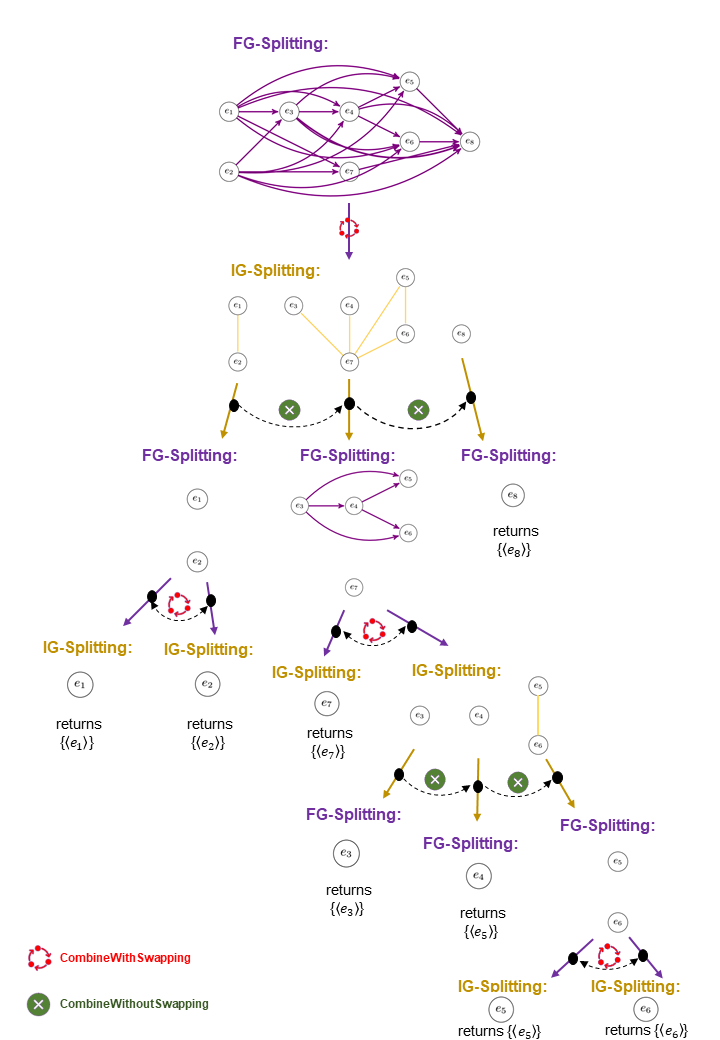
\includegraphics[width=1 \columnwidth]{figures/alg_visualization_paper.png}
	\caption{A visualization of the full recursion tree of the \textsc{ValidPermutations} algorithm when applied on the example event set from Table \ref{table:8 events}.}
	\label{fig: algorithm visualization}
	%width=1\columnwidth
\end{figure}
%
%
%
%
%
%
% 

Fig. \ref{fig: algorithm visualization} provides a visualization of all recursion rounds of Algorithm \ref{alg:valid permutations} on input set $E$ from Table \ref{table:8 events}.
The directed graphs with violet arcs represent the subgraphs induced from the follows graph.
The violet arcs pointing outwards from any violet graph each represent a connected component of that graph.
As we explained earlier, the valid sequences of these violet components are then merged together with swapping.
The red circling lines symbolize the \textsc{CombineWithSwapping} method on these components.
The undirected graphs with yellow edges show the subgraphs induced by the interval graph.
Similarly, the yellow arcs pointing outwards from any yellow graph each represent a connected component of that graph.
The valid sequences from these components are merged back together by preserving a fixed ordering.
The green cross in the visualization symbolizes the cartesian product over those components computed by the \textsc{CombineWithoutSwapping} method.
In this example, the recursion breaks as all subgraphs are split until they consist of single nodes.
The violet and yellow graphs guide the top-down view of the algorithm, starting from the original single follows graph and partitioning the vertex set in each round until we arrive at trivial nodes.
The green cross and the red circle over the arrows connecting different components guide the bottom-up view of the algorithm.
They indicate how valid subsequences are to be merged together in every step, starting from the trivial singleton sequences and ending with the full sequences of size $|E|$.
%
%
%
%
%
%
%Then Algorithm \ref{alg: FollowsGraph Splitting} is called on input $(\mathcal{F}(E),\mathcal{I}(E),E)$.
%$\mathcal{F}(E)$ has only one component, for which Algorithm \ref{alg: IntervalGraph Splitting} is called.
%In lines 4-9, the connected components of the interval graph $\mathcal{I}(E)$ are computed and ordered into $\langle \{e_1,e_2\},\{e_3,e_4,e_5,e_6,e_7\},\{e_8,\} \rangle$.
%Then for each of them, Algorithm \ref{alg: PrecGraph Splitting} is called again with the corresponding vertex subset:\\
%- On component $\{e_1,e_2\}$: $\mathcal{F}[\{e_1,e_2\}]$ has two components, namely the two single nodes.
%When calling Algorithm $\ref{alg: IntervalGraph Splitting}$ on each one of these nodes, the trivial outputs $\{\langle e_1 \rangle\}, \{\langle e_2 \rangle\}$ are yielded.
%In line 9 (Alg. \ref{alg: PrecGraph Splitting}) these two are combined with swapping by Algorithm \ref{alg:combine with} which yields set $\{ \langle e_1, e_2 \rangle, \langle e_2, e_1 \rangle \}$.\\
%- On component $\{e_3,e_4,e_5,e_6,e_7\}$: $\mathcal{F}[\{e_3,...,e_7\}]$ has two connected components, namely $\{e_3,e_4,e_5,e_6\}$ and $\{e_7\}$.
%Algorithm \ref{alg: IntervalGraph Splitting} applied to $\{e_7\}$ yields the trivial set $\{e_7\}$.
%On input $\{e_3,e_4,e_5,e_6\}$, it computed the interval graph and sorts its components into $\langle \{e_3\}, \{e_4\}, \{e_5,e_6\} \rangle$.
%Algorithm \ref{alg: PrecGraph Splitting} applied to the three directed subgraphs induced by these three vertex sets yields (after another round of calling Alg. \ref{alg: IntervalGraph Splitting} and \ref{alg:combine with}) the outputs $\{ \langle e_3 \rangle \}$, $\{ \langle e_4 \rangle \}$ and $\{ \langle e_5,e_6 \rangle, \langle e_6, e_5 \rangle \}$ respectively.
%These three outputs have exactly this order when they are combined without swapping in line 14 of Algorithm \ref{alg: IntervalGraph Splitting}.
%This yields the set $\{ \langle e_3,e_4,e_5,e_6\rangle, \langle e_3,e_4,e_6,e_5 \rangle\}$.
%On a later round, the sets $\{\langle e_3,e_4,e_5,e_6\rangle, \langle e_3,e_4,e_6,e_5 \rangle\}$ and $\{\langle e_7 \rangle\}$ are combined with swapping: In this case, event $e_7$ is put to every possible position of each of the longer lists (\textcolor{red}{lines 10-16}) of Algorithm \ref{alg:combine with} yielding 10 valid permutations.\\
%- On component $\{e_8\}$: Algorithm \ref{alg: IntervalGraph Splitting} yields the trivial set $\{\langle e_8 \rangle\}$.

%In the end, the sets yieled for components $\{e_1,e_2\}$, $\{e_3,e_4,e_5,e_6,e_7\}$ and $\{e_8\}$ are all combined in this order into full sequences of length 8 in line 14 of Algorithm \ref{alg: IntervalGraph Splitting}, yielding in the end the set of all $20 ~ (2 \times 10 \times 1)$ topological sortings of the original $\mathcal{F}(E)$ and this way $\mathcal{R}_e(E)$ conatining:
Applied on the example event set, the \textsc{ValidPermutations} algorithm yields the following 20 sequences:
\begin{itemize}
\item $\langle e_1,e_2,e_3,e_4,e_5,e_6,e_7,e_8\rangle$ 
\item $\langle e_1,e_2,e_3,e_4,e_6,e_5,e_7,e_8\rangle$ 
\item $\langle e_1,e_2,e_3,e_4,e_5,e_7,e_6,e_8\rangle$
\item $\langle e_1,e_2,e_3,e_4,e_6,e_7,e_5,e_8\rangle$ 
\item $\langle e_1,e_2,e_3,e_4,e_7,e_5,e_6,e_8\rangle$
\item $\langle e_1,e_2,e_3,e_4,e_7,e_6,e_5,e_8\rangle$
\item $\langle e_1,e_2,e_3,e_7,e_4,e_5,e_6,e_8\rangle$
\item $\langle e_1,e_2,e_3,e_7,e_4,e_6,e_5,e_8\rangle$
\item $\langle e_1,e_2,e_7,e_3,e_4,e_5,e_6,e_8\rangle$
\item $\langle e_1,e_2,e_7,e_3,e_4,e_6,e_5,e_8\rangle$
\item $\langle e_2,e_1,e_3,e_4,e_5,e_6,e_7,e_8\rangle$ 
\item $\langle e_2,e_1,e_3,e_4,e_6,e_5,e_7,e_8\rangle$ 
\item $\langle e_2,e_1,e_3,e_4,e_5,e_7,e_6,e_8\rangle$
\item $\langle e_2,e_1,e_3,e_4,e_6,e_7,e_5,e_8\rangle$ 
\item $\langle e_2,e_1,e_3,e_4,e_7,e_5,e_6,e_8\rangle$
\item $\langle e_2,e_1,e_3,e_4,e_7,e_6,e_5,e_8\rangle$
\item $\langle e_2,e_1,e_3,e_7,e_4,e_5,e_6,e_8\rangle$
\item $\langle e_2,e_1,e_3,e_7,e_4,e_6,e_5,e_8\rangle$
\item $\langle e_2,e_1,e_7,e_3,e_4,e_5,e_6,e_8\rangle$
\item $\langle e_2,e_1,e_7,e_3,e_4,e_6,e_5,e_8\rangle$
\end{itemize}
%
%
%
%
%
%
%
\section{Complexity Analysis}
The \textsc{ValidPermutations} Algorithm (\ref{alg:valid permutations}) computes the set of correct evaluation orders on the input event set by using the interval graph technique, that is, partitioning the event set into subsets that can be ordered in time and then recursively computing the valid orderings for the smaller event sets.
When computing the interval graph on some given event set partitions it further, then the subsets for which the orderings have to be computed get smaller and smaller.
The recursion breaks on trivial components of size one yielding the trivial singleton sequence.
If the input event set cannot be divided into smaller timely comparable event subsets, then the method relies on the naive \textsc{TopologicalSortings} algorithm (\ref{alg:topo sortings}) to compute the correct evaluation orders on the current event set.
In both scenarios, the recursion breaks at some point and the smaller sequences are merged back together until they yield the full valid sequences.
Thus, the \textsc{ValidPermutations} algorithm always terminates.

It is easy to determine that for the naive method, that is, constructing the follows graph (Algorithm \ref{alg:follows graph}) and then applying the \textsc{TopologicalSortings} method (\ref{alg:topo sortings}) on it, the runtime is $\mathcal{O}(n \cdot n!)$.
Constructing the follows graph in Algorithm \ref{alg:follows graph} requires $\mathcal{O}(n^2)$.
The \textsc{TopologicalSortings} algorithm goes through all possible permutations over the vertex set of the input graph which runs in $\mathcal{O}(n!)$.
Then, it checks validity for every single one of them, which costs $\mathcal{O}(n)$ for going through each vertex and checking whether the current vertex is in the \textit{previous} set.
Thus, the total running time of the naive method is $\mathcal{O}(n^2) + \mathcal{O}(n \cdot n!) = \mathcal{O}(n \cdot n!)$.

Determining the complexity of the \textsc{ValidPermutations} algorithm is not as straighforward, since the runtime heavily depends on the graph structure of the follows graph and whether the algorithm falls back into the naive method or not.
The graph structure affects how well the interval graph technique works on the input event set and how many recursion rounds are completed before termination.
First, we analyze the runtime assuming that the recursion only breaks on trivial components, that is, the naive method is never called.
The visualization of the example run in Fig. \ref{fig: algorithm visualization} can be helpful when conducting this runtime analysis.
A full recursion round consists of calling \textsc{FollowsGraphSplitting} and \textsc{IntervalGraphSplitting} once.
In the visualization, this would consist of a round of a violet and yellow graphs pair.
Computing the initial follows and interval graph in Algorithm \ref{alg:valid permutations} each costs $\mathcal{O}(n^2)$ resulting in $\mathcal{O}(2n^2)$.
In each recusion round, a follows graph and an interval graph are computed, which runs in $\mathcal{O}(2n^2)$, and for each graph, the connected components are detected, which results in an additional $\mathcal{O}(2n^2)$.
Sorting the components in the \textsc{IntervalGraphSplitting} method runs in $\mathcal{O}(n \cdot log(n))$.
In total, these operations contribute to a runtime of $\mathcal{O}(4n^2)+\mathcal{O}(n \cdot log(n)) = \mathcal{O}(n^2)$ for each round.
Suppose $S$ is the set of all valid permutations over the input event set.
Since every $s \in S$ is reconstructed from its subsequences by explicitly dictating only the valid positions for each element from the event set, each valid sequence from $S$ contributes $\mathcal{O}(1)$ in each recusion round.
In total this is $\mathcal{O}(|S|)$.
If $d$ is the maximal recursion depth, then the total runtime is $d \cdot \big(\mathcal{O}(n^2) + \mathcal{O}(|S|) \big) = \mathcal{O}(dn^2 + d|S|)$.
On the other hand, if the recursion breaks by returning to the naive method because that particular subset of the input event set can not be further fragmentized, then there is an added runtime which is asymptotic in the size of that component.
That is why for the general case, the runtime method is $\mathcal{O}(dn^2 + d|S| + k!)$, where $k$ is the size of the biggest component whose valid sequences are determined through the naive method.
The impact of the fallback into the naive method may, however, not be as dramatic if $k$ is a lot smaller than $n$.
Note that regardless of whether the naive method is called at some point, in the worst-case scenario, the runtime is still $\mathcal{O}(n!)$.
If a very high number (close to $n!$) of sequences are valid, then all those sequences will have to be constructed, therefore the $|S|$ term is also very large. 

Next, we show two input examples, one on which the \textsc{ValidPermutations} algorithm performs particularly well compared to the naive method, and one on which its execution is very similar to the naive method. 
%
%
%
%
\begin{figure}[h!]
\centering

	\begin{tikzpicture}[->,>=stealth',shorten >=1pt,node 						distance=2.5cm,auto,main node/.style={circle,draw,align=center}]
	%\draw [help lines] (0,0) grid (7,3);
	\node[main node] (A) at (1,1) {$e_1$};
	\node[main node] (B) at (3,1) {$e_2$};
	\node[main node] (C) at (5,1) {$e_3$};
	\node[main node] (D) at (7,1) {$e_4$};
	\node[main node] (E) at (9,1) {$e_5$};
	
	\path
	(A) edge (B)
	(A) edge [bend right] (C)
	(A) edge [bend right] (D)
	(A) edge [bend right] (E)
	(B) edge (C)
	(B) edge [bend right] (D)
	(B) edge [bend right] (E)
	(C) edge (D)
	(C) edge [bend right] (E)
	(D) edge (E)

	;
	\end{tikzpicture}
	
	\vspace{1cm}
	
	\begin{tikzpicture}[->,>=stealth',shorten >=1pt,node 						distance=2.5cm,auto,main node/.style={circle,draw,align=center}]
	%\draw [help lines] (0,0) grid (7,3);
	\node[main node] (A) at (1,1) {$e_1$};
	\node[main node] (B) at (3,1) {$e_2$};
	\node[main node] (C) at (5,1) {$e_3$};
	\node[main node] (D) at (7,1) {$e_4$};
	\node[main node] (E) at (9,1) {$e_5$};
	
	\path


	;
	\end{tikzpicture}
	\caption{The upper graph shows the follows graph of some uncertain process instance where no event pair has overlapping time intervals.
	The lower graph is the corresponding interval graph.}
	\label{fig: runtime example 1}
\end{figure}
%
%
%
%
%
\begin{figure}[h!]
\centering

	\begin{tikzpicture}[->,>=stealth',shorten >=1pt,node 						distance=2.5cm,auto,main node/.style={circle,draw,align=center}]
	%\draw [help lines] (0,0) grid (10,5);
	\node[main node] (A) at (0,1) {$e_1$};
	\node[main node] (B) at (0,4) {$e_2$};
	\node[main node] (C) at (3,1) {$e_5$};
	\node[main node] (D) at (3,2.5) {$e_4$};
	\node[main node] (E) at (3,4) {$e_3$};
	
	\path
	(A) edge (C)
	(B) edge (C)
	(B) edge (D)
	(B) edge (E)

	;
	%\end{tikzpicture}
	%
	%
	%
	%
	%\begin{tikzpicture}[-,>=stealth',shorten >=1pt,node 						distance=2.5cm,auto,main node/.style={circle,draw,align=center}]
	\node[main node] (A) at (6,1) {$e_1$};
	\node[main node] (B) at (6,4) {$e_2$};
	\node[main node] (C) at (9,1) {$e_5$};
	\node[main node] (D) at (9,2.5) {$e_4$};
	\node[main node] (E) at (9,4) {$e_3$};
	
	\path
	(A) edge [-] (B)
	(A) edge [-] (D)
	(A) edge [-] (E)
	(C) edge [-] (D)
	(C) edge[bend right,-] (E)
	(D) edge [-] (E)
	;
	\end{tikzpicture}
	\caption{The left graph shows the follows graph of some uncertain process instance, whereas the right graph shows its corresponding interval graph.}
	\label{fig: runtime example 2}
\end{figure}
%
%
%
%

Consider the 5 events whose follows and interval graphs are shown in Fig. \ref{fig: runtime example 1}.
Note that the corresponding behavior graph of this event set would be a path, indicating that there is only one valid permutation.
When applied on this example, the \textsc{ValidPermutations} algorithm constructs the graphs from Fig. \ref{fig: runtime example 1} and already during the first recursion round, the  \textsc{IntervalGraphSplitting} method detects the 5 trivial components and orders them.
The unique valid sequence is obtained as a cartesian product from the 5 sets containing the singleton sequences.
In the naive method, the set of topological sortings are computed on the follows graph.
Since there are 5 events, all 5!=120 permutations are considered and checked for validity, even though only one is a topological sorting and thus a correct evaluation order.

Now consider the 5 events in the example from Fig. \ref{fig: runtime example 2} which shows their corresponding follows and interval graph.
After computing both graphs, already in the first recursion round of \textsc{ValidPermutations}, the \textsc{IntervalGraphSplitting} method detects that the interval graph has only one connected component.
This indicates that the event set can not be partitioned into comparable subsets.
At this point, the set of topological sortings is computed using the naive \textsc{TopologicalSortings} method, which goes through all 5!=120 possible permutations, even though                                only 18 of them are correct.   
%
%
%
%
%
%
%\newpage
\section{Runtime Experiments}
Both the naive (Algorithm \ref{alg:topo sortings}) and the novel method (Algorithm \ref{alg:valid permutations}) of obtaining the correct evaluation orders over a set of uncertain events are implemented in Python\footnote{\url{https://github.com/biankabakullari/UncertainLogProbabilities/tree/master/code/Trace_Realizations_Alg}}.
In this section, we show the results of two series of experiments that aim to compare the running times of the new \textsc{ValidPermutations} algorithm and the naive \textsc{TopologicalSortings} method.
In both of them, the input is a set of events represented as triples containing the event ID, the minimum and maximum timestamp.
Each event set is generated the following way: First, we generate a synthetic log containing a single certain trace of a specific length using the PM4Py framework \cite{pm4py}.
More specifically, given a parameter $n$, we first generate a Petri net with $n$ visible transitions which can only replay a single sequence.
Then, we run a simulator on this Petri net to obtain synthetic event data in form of a log containing the unique replayable trace.
To add uncertainty to the data, we use the functionalities provided by the PROVED \cite{proved} library.
More specifically, we make use of a function that given a certain trace and a parameter $p$, randomly generates minimum and maximum timestamp values for the events so that the probability that any two subsequent events overlap is $p$.
Timestamps are represented by their distance from the \textit{Unix Epoch}.
We let both algorithms run on identical events sets and measure the elapsed time for each of them.
The plotted performance results are obtained as an average of 10 runs of the corresponding experiment.

In the first series of experiments, we compare the novel algorithm \textsc{ValidPermutations} with the naive \textsc{TopologicalSortings} method by using an input event set of a fixed length $n=8$, where timestamp uncertainty is generated with increasing probability $p$.
%
%
%
\begin{figure}
	\centering
	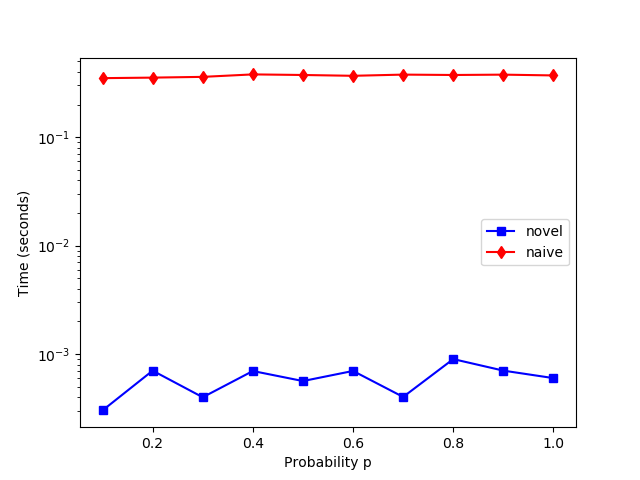
\includegraphics[width=0.8\columnwidth]{figures/n_fixed_8_logscale.png}
	\caption{Time in seconds for computing the correct evaluation orders on a set of 8 events with timestamp uncertainty.}
	\label{fig: series1}
	%width=1\columnwidth
\end{figure}
%
%
%

As expected, the results in Fig. \ref{fig: series1} show that the \textsc{ValidPermutations} Algorithm terminates in a fraction of the time required by the naive method of the \textsc{TopologicalSortings} algorithm.
As we explained before, the new algorithm performs particularly well if the input event set can be partitioned into comparable subsets.
This avoids the asymptotic runtime of checking all possible permutations, most of which are invalid.
In the second series of experiments, the parameter $p$ for generating timestamp uncertainty is kept fixed at either $0.2$ or $0.8$, while the size $n$ of the input event set varies from 1 to 10.
%To generate such event sets with rather few overlappings, we use a probability $p=0.4$ when adding uncertain timestamps to the data and compare the runtime for different input sizes.
%
%
%
\begin{figure}
	\centering
	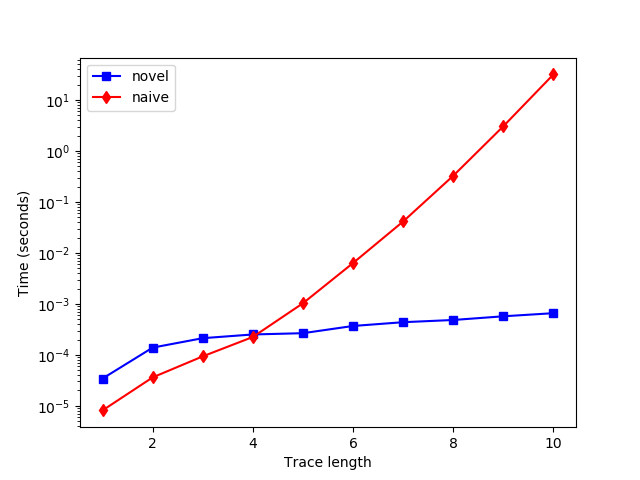
\includegraphics[width=0.8\columnwidth]{figures/fixed_p_08_logscale.png}
	\caption{Time in seconds for computing the correct evaluation orders on an event set of increasing size. The probability of two neighboring events to have overlapping timestamps is $p=0.8$.}
	\label{fig: series21}
	%width=1\columnwidth
\end{figure}
%
%2
%
As expected, Fig. \ref{fig: series21} and \ref{fig: series22} show how the benefit of fragmentizing the input event set to avoid checking all permutations increases dramatically for increasing input size $n$.
Only for very small $n$ ($<4$), the novel method seems to be slower than the naive one, indicating that in such cases, computing the follows and interval graphs is less efficient than checking all possible permutations for validity.
%
%
%
\begin{figure}
	\centering
	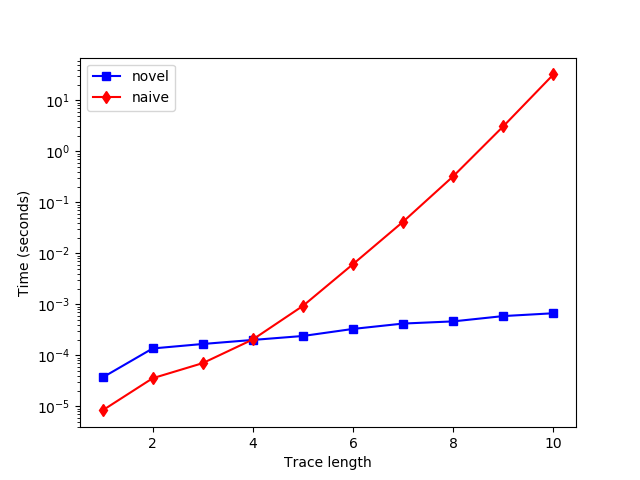
\includegraphics[width=0.8\columnwidth]{figures/fixed_p_02_logscale.png}
	\caption{Time in seconds for computing the correct evaluation orders on an event set of increasing size. The probability of two neighboring events to have overlapping timestamps is $p=0.2$.}
	\label{fig: series22}
	%width=1\columnwidth
\end{figure}
%
%
%
%
%
%
%
%

In summary, our experiments show that the novel algorithm has a much better performance than the naive method and the runtimes between the two differ exponentially with increasing input size.
This might lie on the fact that the function we use to add timestamp uncertainty to the certain data mostly creates timestamp overlappings of neighboring events.
Such uncertain event sets offer a well partitionable input to the novel method, making it less affectable by the input size, whereas the runtime of the naive algorithm still increases exponentially.
While the novel algorithm still might show a runtime in seconds that is noticeably above 0 for larger inputs, the naive method is far too slow on those inputs for its runtime to be plotted meaningfully.
%
%
%
%
%
%\newpage
\section{Event Trace Realizations with Indeterminate Events}
In the previous section, we saw how we can compute a set of valid permutations for any event set $E$.
Note that in the computed valid permutations, every event of $E$ appears in all permutations yielded by the algorithm.
Thus, the computed valid permutations cover all correct evaluation orders on $(E, \prec_{\mathcal{E}})$ if and only if all events in $E$ are determinate.
Otherwise, we have to extend the set of valid permutations by the missing sequences in which indeterminate events do not appear.
This can be done the following way:
Let $E$ be an event set and let $\overline{E}=\{e \in E \mid \pi_o(e) \neq  ~! \vee \big( \pi_o(e)=f_O \in F_{\mathcal{U}_O} \wedge f_O(?) > 0 \big)\}$ denote the set of indeterminate events from $E$.
Similarly, we can indicate indeterminate events by overlining them. 
This way, for every valid permutation $s$ we have computed in Algorithm \ref{alg:valid permutations}, we add the remaining $2^{|\overline{E}|} - 1 $ sequences missing from the event trace realizations. \\ 
%

For example, let $E=\{e_1,\overline{e_2},\overline{e_3},e_4\}$ be some event set and suppose that $\langle e_1,e_2,e_3,e_4 \rangle$ and $\langle e_1,e_3,e_2,e_4 \rangle$ are the valid permutations computed from Algorithm \ref{alg:valid permutations}.
The missing sequences are $\langle e_1, e_2, e_4 \rangle, \langle e_1, e_3, e_4 \rangle$ and $\langle e_1, e_4 \rangle$.
Finally, we update $\mathcal{R}_e(E)$ so that it contains all 5 possible event trace realizations.

From now on, we assume that the computed set $\mathcal{R}_e(E)$ of some event set $E$ already contains all event trace realizations of $E$.
%Besides already having a possibly non-empty set $\overline{E} \subseteq E$ containing the indeterminate events, one can also notice whether the case corresponding to $E$ has indeterminate events by looking at the lengths of the sequences of event trace realizations.
%These sequences have all length $|E|$ when there are no indeterminate events.
%
%
%
%
%
%
%


\chapter{Estimating Probabilities for Trace Realizations}
\label{chap:estimates}
\section{Obtaining Probabilities from Information on Uncertainty}
In this section we obtain probability estimates for all activity trace realizations related to a particular uncertain process instance.
It is important to stress our assumption that the information on uncertainty related to a particular attribute in some event satisfies the following:
It is independent from the uncertainty information on the same attribute present in other events (same attribute different events independence) and it is independent from the uncertainty information on the other attributes of the same event (same event different attributes independence).
As we will see, this assumption underlies the way the probability estimates for the activity trace realizations are obtained in the remainder of this work.

Furthermore, for any given event set of some uncertain process instance we identify its uncertainty type as we explained in Chapter \ref{chap:prelim}.
Then we can treat all events belonging to the same instance as if they had this particular uncertainty type.
This poses no constraint since as we showed in Chapter \ref{chap:prelim}, each attribute value of another uncertainty type can be modified into an equivalent one with the desired uncertainty type.

In the remainder of this section we always assume that for a given case $c$, we are provided with its event set $E$ and the set $\mathcal{R}_e$ containing all possible event trace realizations of case $c$.
From a process point of view, we are rather interested in the activity trace corresponding to the uncertain process instance identified by case $c$.
The set $\mathcal{R}_a$ of possible activity traces must however be obtained from the sets $A(s_e)$ for all $s_e \in \mathcal{R}_e$, that is, the set of activity sequences enabled by each possible event sequence (Def. \ref{def: activity trace realizations}).
From here one can observe that the probability $\textbf{p}(s_a)$ that an activity sequence $s_a \in \mathcal{R}_a$ is indeed the activity trace of case $c$ depends from the set of all event sequences enabling it.

%
%
%
%
%
%
\begin{figure}[h]
	\centering

	\begin{tikzpicture}[->,>=stealth',shorten >=1pt,node 						distance=2.5cm,auto,main node/.style={circle,draw,align=center}]
	%\draw [help lines] (0,0) grid (10,3);
	\node[main node,label=above: \large $a$] (A) at (3,2) {$e_1$};
	\node[main node,label=above: \large ${\{b,c\}}$] (B) at (5,3) {$e_2$};
	\node[main node,label=above: \large ${\{c,d\}}$] (C) at (5,1) {$e_3$};
	\node[main node,label=above: \large $d$] (D) at (7,2) {$e_4$};
	
	\path
	(A) edge (B)
	(A) edge (C)
	(B) edge (D)
	(C) edge (D)
	

	;
	\end{tikzpicture}
	\caption{The two event sequences $\langle e_1,e_2,e_3,e_4 \rangle$ and $\langle e_1,e_3,e_2,e_4 \rangle$ both enable activity sequence $\langle a,c,c,d \rangle$.
	}
	\label{fig: two enablers}
\end{figure}
%
%
%
%
%
%
Figure \ref{fig: two enablers} shows the behavior graph of a process instance containing 4 events.
Both possible event sequences enable a common activity trace.
The more event sequences enable a particular activity trace, the higher its likelihood.
Furthermore, for each such event sequence, one can construct a probability function $P_e(s_e)$ reflecting the likelihood of sequence $s_e$ itself and a probability function $P_a(s_a \mid s_e)$ reflecting the likelihood that the activity trace corresponding to $s_e$ is indeed $s_a$.
The value of $P_e$ is affected from the uncertainty information in timestamps and indeterminate events while the value of $P_a$ is aggregated from the uncertainty information in the activity labels.
We will see some examples for this later.

From now on, we refer to the set of event trace and activity trace realizations with $\mathcal{R}_e$ and $\mathcal{R}_a$ respectively.
Furthermore, for any $s_a \in \mathcal{R}_a$ we define the set 
$ Enablers(s_a):= \{s_e \in \mathcal{R}_e \mid s_a \in A(s_e)\}$ containing the event sequences from $\mathcal{R}_e$ which might have executed activity sequence $s_a$.

Given some activity trace realization $s_a$ of some uncertain process instance and the set of its enablers, its probability is computed as following:
\begin{align*}
\textbf{p}(s_a) = \sum_{s_e \in Enablers(s_a)}P_e(s_e) \cdot P_a(s_a\mid s_e)
\end{align*} 

In the next two subsections we show how $P_e$ and $P_a$ are aggregated from the uncertainty information given on event and attribute level.
For any uncertain process instance with activity trace realizations $\mathcal{R}_a$ it holds that $\sum_{s_a \in \mathcal{R}_a} \textbf{p}(s_a) = 1$ since both $P_e$ and $P_a$ are each constructed to be (independent) probability distributions.
%Also, the multiplication of the $P_e$ and $P_a$ values reflects our assumption that the uncertainty information on any attribute is independent from any uncertainty information on other attributes of the same event. 
The exact equations for $P_e$ and $P_a$ depend on the uncertainty type of the process instance in question.
For this reason, the event set of the uncertain instance must be part of the input of the probability function $\textbf{p}(\cdot)$ together with the activity trace.
For ease of notation, we omit the event set from the signature and assume the uncertainty type of the process instance in question is known or has already been determined.


\subsection{Uncertainty in Activities}
As we mentioned, $P_a(s_a \mid s_e)$ yields the probability that event sequence $s_e$ executes activity sequence $s_a$.
This value can be aggregated from the information on the uncertainty of activity labels.
If there is no uncertainty in activities, then each event has a unique activity label, that is, $\pi_a(e)$ always yields a single label from $\mathcal{U}_A$ for all $e \in s_e$.
Thus the whole event sequence $s_e$ enables a unique activity trace $s_a$ and the value of $P_a(s_a \mid s_e)$ is trivially 1.

This is not the case whenever there is uncertainty in activities.
In that case, each event sequence $s_e \in \mathcal{R}_e$ enables every activity trace from $A(s_e)$ as defined in Chapter \ref{chap:prelim}.

\begin{itemize}
\item
\underline{$[A]_{\mathbb{S}}$}:
If there is strong uncertainty in activities, then each event has a set of possible activity labels and no information on the likelihood of each activity.
For this reason we suppose that each activity is equally possible which in turn implies that every sequence from $A(s_e)$ for any $s_e \in \mathcal{R}_e$ is equally possible.
Precisely, for any $s_e \in \mathcal{R}_e$ and $s_a \in A(s_e)$:
\begin{align*}
P_a(s_a \mid s_e) = \frac{1}{|A(s_e)|}.
\end{align*}

\item
\underline{$[A]_{\mathbb{W}}$}:
If there is weak uncertainty in activities, then for each event $e \in s_e$ and activity label $a \in \pi_a^{set}(e)$ the probability that $e$ executes $a$ is given by $f_A^e(a) \in F_{\mathcal{U}_A}$ where $f_A^e = \pi_a(e)$.
Again, we assume that for all $e \in s_e$, the distributions over their activity sets are independent.
Thus, for every $s_e=\langle e_1,...,e_n \rangle \in \mathcal{R}_e$ and $s_a = \langle a_1,...,a_n \rangle \in A(s_e)$, the value $P_a$ can be easily aggregated from these distributions the following way:
\begin{align*}
P_a(s_a \mid s_e) = \prod_{i=1}^{n} f_A^{e_i}(a_i) 
\end{align*}
\end{itemize}
Figures \ref{fig: activities strong} and \ref{fig: activities weak} show the examples of a process instance with uncertainty in activities.
In the first example (Fig. \ref{fig: activities strong}) we only know the set of possible labels of events $e_2$ and $e_3$.
Here all activity traces enabled by the same event trace are equally possible.
In the second case in Fig. \ref{fig: activities weak} we also know the likelihood of each possible activity label of events $e_2$ and $e_3$.
These values are now taken into consideration when computing the probability that a sequence $s_e$ enables a particular activity trace $s_a \in A(s_e)$.
%
%
%
%
%
\begin{figure}[h]
\centering

	\begin{tikzpicture}[->,>=stealth',shorten >=1pt,node 						distance=2.5cm,auto,main node/.style={circle,draw,align=center}]
	%\draw [help lines] (0,0) grid (7,3);
	\node[main node,label=above: \large $a$] (A) at (1,2) {$e_1$};
	\node[main node,label=above: \large ${\{b,c\}}$] (B) at (3,3) {$e_2$};
	\node[main node,label=above: \large ${\{c,d\}}$] (C) at (5,3) {$e_3$};
	\node[main node,label=above: \large $d$] (D) at (4,1) {$e_4$};
	\node[main node,label=above: \large $e$] (E) at (7,2) {$e_5$};
	
	\path
	(A) edge (B)
	(B) edge (C)
	(A) edge (D)
	(C) edge (E)
	(D) edge (E)
	

	;
	\end{tikzpicture}
	\caption{Example of a process instance with strong uncertainty in activities. 
	Here $\mathcal{R}_e=\{ 
	s_e^1=\langle e_1,e_2,e_3,e_4,e_5 \rangle, 
	s_e^2=\langle e_1,e_2,e_4,e_3,e_5 \rangle, 
	s_e^3=\langle e_1,e_4,e_2,e_3,e_5 \rangle \}$.
	For every $s_a \in A(s_e^1)=\{
	\langle a,b,c,d,e \rangle,
	\langle a,c,c,d,e \rangle,
	\langle a,b,d,d,e \rangle,
	\langle a,c,d,d,e \rangle\}$
	we have $P_a(s_a \mid s_e^1) = 1/4$.	
	}
	\label{fig: activities strong}
\end{figure}
%
%
%
%
%
%
%
%
%
%
\begin{figure}[h] 
\centering

	\begin{tikzpicture}[->,>=stealth',shorten >=1pt,node 						distance=2.5cm,auto,main node/.style={circle,draw,align=center}]
	%\draw [help lines] (0,0) grid (7,3);
	\node[main node,label=above: \large $a$] (A) at (1,2) {$e_1$};
	\node[main node,label=above: \Large ${\substack{b:~0.7 \\ c:~0.3}}$] (B) at (3,3) {$e_2$};
	\node[main node,label=above: \Large ${\substack{c:~0.4 \\ d:~0.6}}$] (C) at (5,3) {$e_3$};
	\node[main node,label=above: \large $d$] (D) at (4,1) {$e_4$};
	\node[main node,label=above: \large $e$] (E) at (7,2) {$e_5$};
	
	\path
	(A) edge (B)
	(B) edge (C)
	(A) edge (D)
	(C) edge (E)
	(D) edge (E)
	

	;
	\end{tikzpicture}
	\caption{Example of a process instance with weak uncertainty in activities.
	Sequence $s_e=\langle e_1,e_2,e_3,e_4,e_5 \rangle \in \mathcal{R}_e$ is a possible event trace.
	For $s_a'=\langle a,b,d,d,e\rangle, s_a''=\langle a,c,c,d,e \rangle \in A(s_e)$ we have
	$P_a(s_a' \mid s_e)=f_A^{e_1}(a) \cdot f_A^{e_2}(b) \cdot f_A^{e_3}(d) \cdot f_A^{e_4}(d) \cdot f_A^{e_5}(e) = 1 \cdot 0,7 \cdot 0,6 \cdot 1 \cdot 1 
	= 0,42$ whereas 
	$P_a(s_a'' \mid s_e)=f_A^{e_1}(a) \cdot f_A^{e_2}(c) \cdot f_A^{e_3}(c) \cdot f_A^{e_4}(d) \cdot f_A^{e_5}(e) = 1 \cdot 0,3 \cdot 0,4 \cdot 1 \cdot 1 
	= 0,12.
	$}
	\label{fig: activities weak}
\end{figure}
%
%
%
%
%

Through the value of $P_a$ we can assess the likelihood that any given event trace executes a particular activity trace.
The next step is to assess the probability of each event trace itself.


\subsection{Timestamp Uncertainty and Indeterminate Events}

In this section we estimate the probability of each event sequence from set $\mathcal{R}_e$.
Depending on the uncertainty in timestamps and indeterminate events, not every event ordering on event set $E$ is equally likely.
For the simple case where there is no uncertainty in timestamps and all events are determinate, there is one unique event sequence.
Trivially we can assign a $P_e$ value of 1 to this sequence.
In the following we go through all uncertainty scenarios that affect the likelihood of the sequences from $\mathcal{R}_e$ for some event set $E$.

\begin{itemize}
\item
$\underline{[O]_{\mathbb{S}}}:$
Since there is no uncertainty in timestamps, all events from $E$ can be totally ordered.
The behavior graph of such process instances is always a path.
Any event from $\overline{E}$ might have happened or not, but there is no information on which is more likely.
Thus, we view each sequence $s_e$ from $\mathcal{R}_e$ as equally possible:
\begin{align*}
P_e(s_e) = \frac{1}{|\mathcal{R}_e|} = \frac{1}{2^{|\overline{E}|}}.
\end{align*}

\item
$\underline{[O]_{\mathbb{W}}}:$
Since there is no uncertainty in timestamps, all events from $E$ can be totally ordered.
For any event $\overline{e} \in \overline{E}$, the function $f_O^{\overline{e}}$ yields how likely or unlikely it is that the event really happened.
For each sequence $s_e$ from $\mathcal{R}_e$ we define:
\begin{align*}
P_e(s_e) = \prod_{\substack{\overline{e} \in \overline{E}: \\ \overline{e} \in s_e}} f_O^{\overline{e}}(!)
\prod_{\substack{\overline{e} \in \overline{E}: \\ \overline{e} \not \in s_e}} f_O^{\overline{e}}(?).
\end{align*}

%
%
%
%
%
\begin{figure}[h]
\centering

	\begin{tikzpicture}[->,>=stealth',shorten >=1pt,node 						distance=2.5cm,auto,main node/.style={circle,draw,align=center}]
	%\draw [help lines] (0,0) grid (7,3);
	\node[main node] (A) at (1,1) {$e_1$};
	\node[main node,dashed] (B) at (3,1) {$e_2$};
	\node[main node] (C) at (5,1) {$e_3$};
	\node[main node,dashed] (D) at (7,1) {$e_4$};
	
	\path
	(A) edge (B)
	(B) edge (C)
	(C) edge (D)
	

	;
	\end{tikzpicture}
	\caption{The behavior graph of a process instance with indeterminate events. 
	Here $\overline{E} = \{e_2,e_4\}$ and there are four ($4=2^{|\overline{E}|}$) possible event traces: 
	$\mathcal{R}_e = \langle e_1,e_2,e_3,e_4\rangle, 
	\langle e_1,e_2,e_3\rangle, 
	\langle e_1,e_3,e_4\rangle, $ and
	$\langle e_1,e_3\rangle $.
	For each of those sequences $s_e \in \mathcal{R}_e$ we have $P_e(s_e)=1/4$.}
	\label{fig: strong indeterminate}
\end{figure}
%
%
%
%
%
%
%
%
%
%
\begin{figure}[h]
\centering

	\begin{tikzpicture}[->,>=stealth',shorten >=1pt,node 						distance=2.5cm,auto,main node/.style={circle,draw,align=center}]
	%\draw [help lines] (0,0) grid (7,3);
	\node[main node] (A) at (1,1) {$e_1$};
	\node[main node,dashed,label=above: ${!:0.6, ~?:0.4}$] (B) at (3,1) {$e_2$};
	\node[main node] (C) at (5,1) {$e_3$};
	\node[main node,dashed,label=above: ${!:0.2, ~?:0.8}$] (D) at (7,1) {$e_4$};
	
	\path
	(A) edge (B)
	(B) edge (C)
	(C) edge (D)
	

	;
	\end{tikzpicture}
	\caption{Example of a process instance with indeterminate events $e_2$ and $e_4$ where there is information on the likelihood of their occurrence.
	Here we have $P_e(\langle e_1,e_2,e_3,e_4\rangle)=
	f_O^{e_1}(!) \cdot f_O^{e_2}(!) \cdot f_O^{e_3}(!) \cdot f_O^{e_4}(!)
	= 1 \cdot 0,6 \cdot 1 \cdot 0,2 = 0,12$ whereas 
	$P_e(\langle e_1,e_3\rangle)=
	f_O^{e_1}(!) \cdot f_O^{e_2}(?) \cdot f_O^{e_3}(!) \cdot f_O^{e_4}(?) 		= 1 \cdot 0,4 \cdot 1 \cdot 0,8 = 0,32$.}
	\label{fig: weak indeterminate}
\end{figure}
%
%
%
%
%
Figures \ref{fig: strong indeterminate} and \ref{fig: weak indeterminate} show two small examples for these scenarios.


\item
$\underline{[T]_{\mathbb{S}}}:$
In this scenario, all events are determinate but they might be only partially ordered.
Events with overlapping timestamps might have happened in any order and we only know the time interval for every event.
Here one has two alternatives on how to assess the likelihood of each ordering of events. 
One can view each ordering of overlapping events as equally possible.
This leads to $P_e$ assigning probability $\frac{1}{|\mathcal{R}_e|}$ to every $s_e \in \mathcal{R}_e$.
The other alternative arises from the assumption that from a possible time interval $[t_{min}(e), t_{max}(e)]$ of an event $e$ where $t_{min}(e) < t_{max}(e)$, one can conclude that the probability that event $e$ happened at some time $t \in [t_{min(e)}, t_{max}(e)]$ is $\frac{1}{t_{max}(e) - t_{min}(e)}$.
In this case, the strong uncertainty in timestamps is viewed as a special case of weak uncertainty where the distributions on time intervals are always uniform.
The calculation of $P_e$ can be therefore taken from the $[T]_{\mathbb{W}}$ scenario analyzed below.
Figure \ref{fig: strong timestamp} shows the same process instance as Figure \ref{fig: activities strong} as an example of a process instance with strong uncertainty in timestamps where each event is determinate.
%
%
%
%
%
\begin{figure}[h]
\centering

	\begin{tikzpicture}[->,>=stealth',shorten >=1pt,node 						distance=2.5cm,auto,main node/.style={circle,draw,align=center}]
	%\draw [help lines] (0,0) grid (7,3);
	\node[main node] (A) at (1,2) {$e_1$};
	\node[main node] (B) at (3,3) {$e_2$};
	\node[main node] (C) at (5,3) {$e_3$};
	\node[main node] (D) at (4,1) {$e_4$};
	\node[main node] (E) at (7,2) {$e_5$};
	
	\path
	(A) edge (B)
	(B) edge (C)
	(A) edge (D)
	(C) edge (E)
	(D) edge (E)
	

	;
	\end{tikzpicture}
	\caption{Behavior graph of a process instance where there is strong uncertainty in timestamps and all events are determinate. Here we have $\mathcal{R}_e=\{ 
	\langle e_1,e_2,e_3,e_4,e_5 \rangle, 
	\langle e_1,e_2,e_4,e_3,e_5 \rangle, 
	\langle e_1,e_4,e_2,e_3,e_5 \rangle \}$ and each sequence has probability $1/3$.}
	\label{fig: strong timestamp}
\end{figure}
%
%
%
%
%
\item
$\underline{[T]_{\mathbb{W}}}:$
In this scenario, all events are determinate but they are only partially ordered.
Events with overlapping timestamps might have happened in any order and for every event $e$, the value of $f_T^e(t)$ yields the probability that event $e$ happened on timestamp $t$.
This value is always 0 for all $t < t_{min}(e)$ and $t > t_{max}(e)$ (by definition of $t_{min}$ and $t_{max}$ in the weak uncertainty scenario).
Here we make use of this information by making the natural assumption that a particular order between any two overlapping events is more likely if the interval of one event lies further in the future than the other one's, or if the spikes in their timestamp distributions appear in a certain order.
Moreover, since the universe of timestamps is a continuous set, there is always an infinite number of timestamp values each picked from some time interval, such that their odering induces the same ordering of the corresponding events.
For this reason, the value of $P_e$ is assessed as precisely as possible by using integrals.
For a sequence $s_e=\langle e_1,...,e_n \rangle \in \mathcal{R}_e$, let $a_i:=t_{min}(e_i)$ and $b_i:=t_{max}(e_i)$ for all $1 \leq i \leq n$.
Then we define:
\begin{align*}
I(s_e) &= \int_{a_1}^{min\{b_1,...,b_n\}} f_T^{e_1}(x_1)
\int_{max\{a_2,x_1\}}^{min\{b_2,...,b_n\}} f_T^{e_2}(x_2)
\cdot \cdot \cdot \\
&
\int_{max\{a_i,x_{i-1}\}}^{min\{b_i,...,b_n\}} f_T^{e_i}(x_i)
\cdot \cdot \cdot 
\int_{max\{a_n,x_{n-1}\}}^{b_n} f_T^{e_n}(x_n) ~
d_{x_n} ... d_{x_1} \\
&=
\int_{a_1}^{min\{b_1,...,b_n\}} 
\int_{max\{a_2,x_1\}}^{min\{b_2,...,b_n\}} 
\cdot \cdot \cdot 
\int_{max\{a_i,x_{i-1}\}}^{min\{b_i,...,b_n\}} 
\cdot \cdot \cdot 
\int_{max\{a_n,x_{n-1}\}}^{b_n} \\
&
\prod_{i=1}^{n} f_T^{e_i}(x_i) ~
d_{x_n} ... d_{x_1}.
\end{align*}

Note that the value of $I(s_e)$ sums the probabilities of all timestamp values $x_1,...,x_n$ for events $e_1,...,e_n$ where the events have happened in the order given by $s_e$, that is: $x_1 \leq ... \leq x_n$.
For the timestamps to satisfy the inequalities $x_1 \leq  ...  \leq x_n$ where each $x_i$ yields some possible timestamp of event $e_i$, each $e_i$ can only start after event $e_{i-1}$ has finished (except $e_1$ which can start at $a_1$).
Thus the minimal possible value for $x_i$ is $max\{a_i,x_{i-1}\}$.
Also, event $e_i$ has to finish early enough so that the rest of the future events can still happen.
Therefore the maximal possible value for $x_i$ is $min\{b_i,...,b_n\}$.
Note that one can calculate the value of $I$ for any possible ordering from $\mathcal{S}_E$.
However, $I(s_e)=0$ if $s_e \not \in \mathcal{R}_e$.
In this scenario we set $P_e(s_e)= I(s_e)$ for all $s_e \in \mathcal{R}_e$.

The integral values for the event orderings were computed using \texttt{scipy.integrate.nquad} in Python.
We implemented a method which enables generating events with uniform and normal distributions, and then automatically orders the generated pdfs in an arguments' list which is then fed to the \texttt{nquad} method of \texttt{scipy}. 
%
%
%
\begin{table}[h]
\caption{Example of an event set with weak uncertainty on timestamps where the distributions are all uniform over the time intervals.}
	\centering
	\begin{tabular}{ccc}
		\textbf{Case ID} & \textbf{Event ID} & \textbf{Timestamp} \\ \hline
	%\multicolumn{1}{c}{\cellcolor{black!30}\textbf{Case ID}} & 
  %\multicolumn{1}{c}{\cellcolor{black!30}\textbf{Event ID}} &
  %\multicolumn{1}{c}{\cellcolor{black!30}\textbf{Timestamp}}
  %\\\hline
	\multicolumn{1}{|c|}{2133} & 
	\multicolumn{1}{|c|}{$e_1$} &
  	\multicolumn{1}{c|}{\begin{tabular}[c]{@{}c@{}} $U$(11-12-2020 12:00, 11-12-2020 14:00) \end{tabular}} 
\\ \hline
	\multicolumn{1}{|c|}{2133} & 
	\multicolumn{1}{|c|}{$e_2$} &
	\multicolumn{1}{c|}{\begin{tabular}[c]{@{}c@{}}$U$(11-12-2020 15:00, 11-12-2020 17:00)\end{tabular}}                                                                                        \\ \hline
	\multicolumn{1}{|c|}{2133} & 
	\multicolumn{1}{|c|}{$e_3$} &
    \multicolumn{1}{c|}{\begin{tabular}[c]{@{}c@{}}$U$(11-12-2020 18:00, 11-12-2020 20:00)\end{tabular}}                                                                                        \\ \hline
	\multicolumn{1}{|c|}{2133} & 
	\multicolumn{1}{|c|}{$e_4$} &
	\multicolumn{1}{c|}{\begin{tabular}[c]{@{}c@{}}$U$(11-12-2020 16:00, 11-12-2020 19:00)\end{tabular}}                                                                                          \\ \hline
	\multicolumn{1}{|c|}{2133} & 
	\multicolumn{1}{|c|}{$e_5$} &
    \multicolumn{1}{c|}{\begin{tabular}[c]{@{}c@{}}$U$(11-12-2020 20:00, 11-12-2020 21:00) \end{tabular}}                                                                                     \\ \hline
		
	\end{tabular}
	\label{table: weak timestamps}
\end{table} 
%
%
%

To illustrate this with an example, consider the event set shown in Table \ref{table: weak timestamps}.
Each of the events has a possible time interval and the probability distribution on each interval follows a uniform one.
The distribution of the events in time is nicely visualized in the gantt chart in Figure \ref{fig: gantt}. 
%
%
%
\begin{figure}
	\centering
	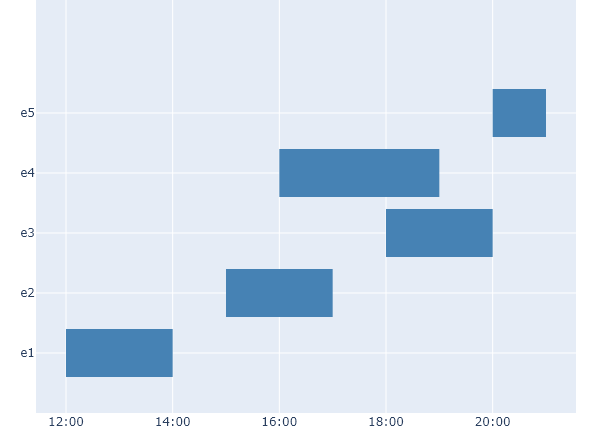
\includegraphics[width=0.8\columnwidth]{figures/gantt_thesis.png}
	\caption{The Gantt chart of the uncertain process instance from Table \ref{table: weak timestamps}.}
	\label{fig: gantt}
	%width=1\columnwidth
\end{figure}
%
%
%
The behavior graph of this event set is the same as the one in Figure \ref{fig: strong timestamp}.
Whether the uncertainty in timestamps is weak or strong does not affect the behavior graph since the latter only captures which events overlap with each other.
As we will see in this example, however, weak uncertainty in timestamps may lead to a probability distribution over the possible event sequences that is much different from a uniform distribution.
A uniform distribution is what we assume when we have strong uncertainty in timestamps and make the decision to consider all event sequences equally likely.

Figure \ref{fig: weak timestamp} visualizes the behavior graph for the event set together with their possible time intervals.
Note that here we have mapped the set of timestamps to a set of numbers.
This is an equivalent transformation regarding the calculation of the probabilities from $I$ since they are only affected from the relative time distances between the lower and upper bounds of the overlapping time intervals.
%
%
%
\begin{figure}[h] 
\centering

	\begin{tikzpicture}[->,>=stealth',shorten >=1pt,node 						distance=2.5cm,auto,main node/.style={circle,draw,align=center}]
	%\draw [help lines] (0,0) grid (7,3);
	\node[main node,label=above:  {$[0,2]$}] (A) at (1,2) {$e_1$};
	\node[main node,label=above:  {$[3,5]$}] (B) at (3,3) {$e_2$};
	\node[main node,label=above:  {$[6,8]$}] (C) at (5,3) {$e_3$};
	\node[main node,label=above:  {$[4,7]$}] (D) at (4,1) {$e_4$};
	\node[main node,label=above:  {$[8,9]$}] (E) at (7,2) {$e_5$};
	
	\path
	(A) edge (B)
	(B) edge (C)
	(A) edge (D)
	(C) edge (E)
	(D) edge (E)
	

	;
	\end{tikzpicture}
	\caption{ Behavior graph of event set from Table \ref{table: weak timestamps} where the extremes of the time intervals are mapped to a set of numbers.
	}
	\label{fig: weak timestamp}
\end{figure}
%
%
As we already saw in the previous example, for this case the set of possible event sequences is $\mathcal{R}_e = \{
\langle e_1,e_2,e_3,e_4,e_5\rangle,
\langle e_1,e_2,e_4,e_3,e_5\rangle,
\langle e_1,e_4,e_2,e_3,e_5\rangle
\}$.
By computing the values of the integrals in $I$ as defined, we obtain  $P_e(\langle e_1,e_2,e_3,e_4,e_5\rangle) = P_e(\langle e_1,e_4,e_2,e_3,e_5 \rangle) \simeq 0.0833$,
while the second sequence is highly more likely with $P_e(\langle e_1,e_2,e_4,e_3,e_5 \rangle) \simeq 0.8333$.
The variance in the probability estimates for the three possible event traces is not surprising since according to the Gantt chart in Figure \ref{fig: gantt}, the trace where event $e_4$ happens between $e_2$ and $e_3$ seems the most likely one. 

%
%
%
Note that the value of $I$ is 0 as soon as one of the events has a certain timestamp as a result of the lower and upper bound of the integral having the same value.
\footnote{Whenever we have certain timestamps, to avoid the integral taking value 0 for every ordering, we can also change the $t_{max}$ value into $t_{max}+\varepsilon$ where $\varepsilon > 0$ is a very small value, e.g. $10^{-10}$.}
\definecolor{mygray}{gray}{0.3}
%\textcolor{mygray}{
However, the equation for computing the integral can be modified to also consider certain timestamps. 
%The integrals in this case go only over the events with uncertain timestamps, while the certain timestamps affect the lower and upper bounds.
The intuition is the following: The timestamp has more than one possible value only for the events with uncertainty in timestamps.
For this reason we do not need to use a variable $x$ in the interval equation for the events with certain timestamps, since its value is fixed.
For a given event sequence we construct the equation just as before but we exclude the events with certain timestamps.
The positions of the events with certain timestamps in the sequence indicate however when the other events are allowed to start and end, thereby affecting the lower and upper bounds of the integrals.
Each event having a variable in the integral has to satisfy an additional condition:
it can only happen both after the last certain event appearing before it in the sequence, and before the first certain event appearing after it in the sequence.
In the following we formalize this idea.\\
For a given event set $E$ of size $n$ let 
$E^{CT} = \{e \in E \mid t_{min}(e) = t_{max}(e)\}$
be the set of events of $E$ with a certain timestamp.
Let $CT = \{t_{min}(e) \mid e \in E^{CT}\}$ be the set of the certain timestamps of events in $E^{CT}$.
Suppose $s_e=\langle e_1,...,e_n \rangle \in \mathcal{R}_e$ is a possible event ordering for which we want to estimate $I(s_e)$.
For every event $e_j \in s$ with $j \in \{1,...,n\}$ such that $e_j \in E \setminus E_{CT}$, we define the following sets:
\begin{align*}
before(e_j) &= \{t \in CT \mid t=t_{min}(e_i) \text{ for some } e_i \in s_e, ~ s.t. ~ e_i \in E_{CT} \wedge i<j\} \\
after(e_j) &= \{t \in CT \mid t=t_{min}(e_i) \text{ for some } e_i \in s_e, ~ s.t. ~ e_i \in E_{CT} \wedge i>j\}.
\end{align*}
From these sets we can obtain two values: 
\begin{align*}
ts^*_{before}(e_j) &= \begin{cases}
	max\{t \in before(e_j)\} & \mbox{if} \; before(e_j) \neq \emptyset,\\
	t_{min}(e_j) & \mbox{otherwise}, \; 
	\end{cases} \\
	%\text{ and } \\
ts^*_{after}(e_j) &= \begin{cases}
	min\{t \in after(e_j)\} & \mbox{if} \; after(e_j) \neq \emptyset,\\
	t_{max}(e_j) & \mbox{otherwise}. \; 
	\end{cases} \\
\end{align*}
Here $ts^*_{before}(e_j)$ yields the certain timestamp of the last event from $E_{CT}$ that appears before $e$ in the ordering, while $ts^*_{after}(e_j)$ yields the certain timestamp of the first event from $E_{CT}$ that appears after $e$ in the ordering.\\
To obtain the probability of having a particular event ordering $s_e \in \mathcal{R}_e$, we first obtain the subsequence $s_e'\sqsubseteq s_e$ such that $s_e' = s_e \downharpoonright_{E \setminus E^{CT}}$, that is, the projection of $s_e$ onto the events with uncertain timestamps.
For $s_e'=\langle e'_1,...,e'_m \rangle$ we compute:
\begin{align*}
I(s_e') &= \int_{max\{a'_1,ts^*_{before}(e'_1)\}}^{min\{b'_1,...,b'_m,ts^*_{after}(e'_1)\}} f_T^{e'_1}(x_1)
\int_{max\{a'_2,x_1,ts^*_{before}(e'_2)\}}^{min\{b'_2,...,b'_m,ts^*_{after}(e'_2)\}} f_T^{e'_2}(x_2)
\cdot \cdot \cdot \\
&
\int_{max\{a'_i,x_{i-1},ts^*_{before}(e'_i)\}}^{min\{b'_i,...,b'_m,ts^*_{after}(e'_i)\}} f_T^{e_i}(x_i)
\cdot \cdot \cdot 
\int_{max\{a'_m,x_{m-1},ts^*_{before}(e'_m)\}}^{b'_m,ts^*_{after}(e'_m)} f_T^{e'_m}(x_m) ~\\
&
d_{x_m} ... d_{x_1} \\
&=
\int_{max\{a'_1, ts^*_{before}(e'_1)\}}^{min\{b'_1,...,b'_m,ts^*_{after}(e'_1)\}}
\int_{max\{a'_2,x_1,ts^*_{before}(e'_2)\}}^{min\{b'_2,...,b'_m,ts^*_{after}(e'_2)\}}
\cdot \cdot \cdot \\
&
\int_{max\{a'_i,x_{i-1},ts^*_{before}(e'_i)\}}^{min\{b'_i,...,b'_m,ts^*_{after}(e'_i)\}}
\cdot \cdot \cdot 
\int_{max\{a'_m,x_{m-1},ts^*_{before}(e'_m)\}}^{b'_m} \\
&
\prod_{i=1}^{m} f_T^{e'_i}(x_i) ~
d_{x_m} ... d_{x_1}.
\end{align*}
To make this clear we use an example.
%
%
%
\begin{figure}[h] 
\centering
	\begin{tikzpicture}[->,>=stealth',shorten >=1pt,node 						distance=2.5cm,auto,main node/.style={circle,draw,align=center}]
	%\draw [help lines] (0,0) grid (7,3);
	\node[main node,label=above:  {$[0,2]$}] (A) at (1,2) {$e_1$};
	\node[main node,label=above:  {$5$}] (B) at (3,3) {$e_2$};
	\node[main node,label=above:  {$[6,8]$}] (C) at (5,3) {$e_3$};
	\node[main node,label=above:  {$[4,7]$}] (D) at (4,1) {$e_4$};
	\node[main node,label=above:  {$9$}] (E) at (7,2) {$e_5$};	
	\path
	(A) edge (B)
	(B) edge (C)
	(A) edge (D)
	(C) edge (E)
	(D) edge (E);
	\end{tikzpicture}
	\caption{Behavior graph of an uncertain process instance. Events $e_2$ and $e_5$ have a certain timestamp.}
	\label{fig: weak timestamp modified}
\end{figure}
In Figure \ref{fig: weak timestamp modified} we have $E=\{e_1,e_2,e_3,e_4,e_5\}$, $E^{CT}=\{e_2,e_5\}$ and $CT=\{t_{min}(e_2),t_{min}(e_5)\} \allowbreak = \{5,9\}$.
Suppose we want to compute the probability $P_e$ of sequence $s=\langle e_1,e_4,e_2,e_3,e_5\rangle$.
First we obtain the following values:
$ts^*_{before}(e_1)=t_{min}(e_1)=0,
ts^*_{after}(e_1)=min\{5,9\}=5,
ts^*_{before}(e_3)=max\{5\}=5,
ts^*_{after}(e_3)=min\{9\}=9,
ts^*_{before}(e_4)=t_{min}(e_4)=4,
ts^*_{after}(e_4)=min\{5,9\}=5.$
Then we estimate $I(s')$ where $s'=\langle e_1,e_4,e_3\rangle$ is the projection of $s$ onto the set of events with uncertain timestamps.
\begin{align*}
I(s'=\langle e_1,e_4,e_3\rangle) &= 
\int_{min\{a_1,ts^*_{before}(e_1)\}}^{min\{b_1,b_3,b_4,ts^*_{after}(e_1)\}} f_T^{e_1}(x_1)
\int_{max\{a_4,x_1,ts^*_{before}(e_4)\}}^{min\{b_3,b_4,ts^*_{after}(e_4)\}} f_T^{e_4}(x_4) \\
&
\int_{max\{a_3,x_4,ts^*_{before}(e_3)\}}^{min\{b_3,ts^*_{after}(e_3)\}} f_T^{e_3}(x_3) \;
d_{x_3} d_{x_4} d_{x_1} \\
&=
\int_{a_1}^{b_1} f_T^{e_1}(x_1)
\int_{a_4}^{ts^*_{after}(e_4)} f_T^{e_4}(x_4) 
\int_{max\{a_3,x_4\}}^{b_3} f_T^{e_3}(x_3) \;
d_{x_3} d_{x_4} d_{x_1} \\
&=
\int_{a_1}^{b_1} f_T^{e_1}(x_1)
\int_{a_4}^{ts^*_{after}(e_4)} f_T^{e_4}(x_4) 
\int_{a_3}^{b_3} f_T^{e_3}(x_3) \;
d_{x_3} d_{x_4} d_{x_1} \\
&=
\int_{a_4}^{ts^*_{after}(e_4)} f_T^{e_4}(x_4) \; d_{x_4} 
= \int_4^5 1/|7-4| \; d_{x_4} \\
&= 1/3.
\end{align*}
Thus $P_e(s)=I(s')=1/3$. 

%}\\ %for textcolor
%
%
%
%
When both uncertainty in timestamps and indeterminate events are present, the sequences in $\mathcal{R}_e$ contain events which appear in different orders and also events which do not appear in all sequences.
%There are $2^{|\overline{E}|}$ distinct event sequences where $\overline{E} ~ (\subseteq E)$ is the set of indeterminate events.
For an event trace $s_e$, its probability is aggregated from the two following values:
\begin{itemize}
\item the probability that the event trace contains the corresponding specific set of events, which is determined by the uncertainty information on the event type 
\item the probability that the corresponding set of events appears in the given particular order, which is determined by the timestamp intervals and if applicable, the distributions over them. 
\end{itemize}
Multiplying the two values obtained above to yield a probability estimate for the event sequence reflects our assumption that timestamp and event type uncertainty are independent.


\item
$\underline{[T,O]_{\mathbb{S}}}$:
In this scenario, strong uncertainty in the event type indicates that the occurrings vs. non-occurrings of indeterminate events are equally likely.
On the other hand, strong uncertainty in timestamps indicates that all event sequences which contain the same events but in different orders are equally likely.
For $k:=2^{|\overline{E}|}$, one can partition $\mathcal{R}_e$ into $k$ non-empty disjoint sets: $\mathcal{R}_e = S_1 \cup ... \cup S_k$ such that for each $S_i$ with $1 \leq i \leq k$ it holds that $\forall s_e, s_e' \in S_i: ~ set(s_e) = set(s_e')$.
In other words, the event sequences in the same subset contain the same events.
Note that when there are no indeterminate events (as in case $[T]_{\mathbb{S}}$) we have $k=1$ because each sequence in $\mathcal{R}_e$ contains all events from $E$.
Otherwise $k = 2^{\overline{E}}$ because each indeterminate events either appears in the sequence or not.
From hereon, we aggregate the probability estimate for any event sequence $s_e \in S_i \subseteq \mathcal{R}_e$ for all $1 \leq i \leq k$:
\begin{align*}
P_e(s_e) = \frac{1}{|S_i|} \cdot \frac{1}{k}.
\end{align*}
Note that 
\begin{align*}
\sum_{s_e \in \mathcal{R}_e} P_e(s_e) = \sum_{i=1}^k \sum_{s_e \in S_i} P_e(s_e) = \sum_{i=1}^k \frac{1}{k} = 1,
\end{align*}
so $P_e$ describes a probability distribution over the set $\mathcal{R}_e$.
The coefficient $\frac{1}{k}$ reflects the assumption that all sets $S_i$ are equally likely from the uncertain event type point of view.
The coefficient $\frac{1}{|S_i|}$ reflects the assumption that given a particular set of events, all possible orderings between them are equally likely.

Consider the small example from Figure \ref{fig: strong timestamp and qualifier}.
It shows three events with pairwise overlapping time intervals.
Since every ordering on the three events is a correct evaluation order, there are $3!=6$ event sequences containing all three events, and $2!=2$ event sequences of length 2 where the indeterminate event $e_2$ does not appear.
Note that $k=2^1=2$.
We can partition $\mathcal{R}_e = S_1 \cup S_2$ where $S_1$ contains the 6 sequences where all three events appear, and $S_2$ contains the two sequences where $e_2$ is not executed.
For $\langle s_1,s_2,s_3 \rangle \in S_1$ we have $P_e(\langle s_1,s_2,s_3 \rangle) = \frac{1}{6} \cdot \frac{1}{2} = \frac{1}{12}$, whereas for $\langle s_1,s_3 \rangle \in S_2$ we have $P_e(\langle s_1,s_3 \rangle) = \frac{1}{2} \cdot \frac{1}{2} = \frac{1}{4}$.

If it is reasonable to interpret the strong uncertainty in timestamps as weak uncertainty with uniform distributions, then the computation of $P_e$ can be obtained from the $[T]_{\mathbb{W}}[O]_{\mathbb{S}}$ scenario.
%
%
%
%
%
\begin{figure}[h]
\centering

	\begin{tikzpicture}[->,>=stealth',shorten >=1pt,node 						distance=2.5cm,auto,main node/.style={circle,draw,align=center}]
	%\draw [help lines] (0,0) grid (7,3);
	\node[main node] (A) at (2,2) {$e_1$};
	\node[main node,dashed] (B) at (4,2) {$e_2$};
	\node[main node] (C) at (6,2) {$e_3$};

	\path
	
	

	;
	\end{tikzpicture}
	\caption{Behavior graph of a process instance with 3 pairwise overlapping events. Event $e_2$ in addition is indeterminate.
	In this case there are 8 event trace realizations, 6 of length three and 2 of length two.}
	\label{fig: strong timestamp and qualifier}
\end{figure}
%
%
%
%
%

\item
$\underline{[T]_{\mathbb{S}}[O]_{\mathbb{W}}}$:
In contrast to the scenario above, we do not have to assume a uniform distribution across the sets $S_i$ partitioning $\mathcal{R}_e$ as we described before, since there is explicit information on the probability of the occurrence of each event.
Therefore, for any $s_e \in S_i \subseteq \mathcal{R}_e$ where $1 \leq i \leq k$ and $k := 2^{|\overline{E}|}$, we determine:
\begin{align*}
P_e(s_e) = \frac{1}{|S_i|} \cdot \prod_{\substack{\overline{e} \in \overline{E}: \\ \overline{e} \in s_e}} f_O^{\overline{e}}(!)
\prod_{\substack{\overline{e} \in \overline{E}: \\ \overline{e} \not \in s_e}} f_O^{\overline{e}}(?).
\end{align*} 
Consider the example from Figure \ref{fig: strong timestamp weak qualifier}, which is very similar to the last one from Figure \ref{fig: strong timestamp and qualifier}, with the exception that the probability of $e_2$ ocurring is 0.3.
In this case, we have $P_e(\langle e_1,e_2,e_3 \rangle) = \frac{1}{6} \cdot 1 \cdot 0.3 \cdot 1 = 0.05$, whereas $P_e(\langle e_1,e_3 \rangle) = \frac{1}{2} \cdot 1 \cdot 0.7 \cdot 1 = 0.35$.

Again, if it is reasonable to interpret the strong uncertainty in timestamps as weak uncertainty with uniform distributions, then the computation of $P_e$ can be obtained from the $[T,O]_{\mathbb{W}}$ scenario. \\
%
%
%
%
%
\begin{figure}[h]
\centering

	\begin{tikzpicture}[->,>=stealth',shorten >=1pt,node 						distance=2.5cm,auto,main node/.style={circle,draw,align=center}]
	%\draw [help lines] (0,0) grid (7,3);
	\node[main node] (A) at (2,2) {$e_1$};
	\node[main node,dashed,label=above:  \Large $\substack{!:~ 0.3 \\ ?:~0.7}$] (B) at (4,2) {$e_2$};
	\node[main node] (C) at (6,2) {$e_3$};

	\path
	
	

	;
	\end{tikzpicture}
	\caption{Behavior graph of a process instance with 3 pairwise overlapping events. Event $e_2$ occurrs with probability $0.3$.
	In this case there are 8 event trace realizations, 6 of length three and 2 of length two.}
	\label{fig: strong timestamp weak qualifier}
\end{figure}
%
%
%
%
%
%
%
\item
$\underline{[T]_{\mathbb{W}}[O]_{\mathbb{S}}}$:
In this scenario, there is information on the distribution of the timestamp values for each event.
Additionally, some events are indeterminate.
In order for $P_e$ to reflect the probability of each sequence $s_e \in \mathcal{R}_e$ as precisely as possible, we must include the value of $I(s_e)$ while also taking into account that each indeterminate event from $\overline{E}$ might have happened or not.
Again, we partition the set $\mathcal{R}_e = S_1 \cup ... \cup S_k$ where $k=2^{|\overline{E}|}$ such that the sequences in each set $S_i$ contain exactly the same events.
For every set $S_i$, the integral $I$ yields a probability distribution over the event sequences present in $S_i$.
Because of indeterminate events there are $k$ such sets.
Since there is no information on the likelihood of indeterminate events,  we want to view the sequences across sets as equally likely w.r.t the event set they contain.
Thus we multiply constant $1/k$ to the values yielded by each $I$.
More precisely, for any $s_e \in \mathcal{R}_e$ we define:
\begin{align*}
P_e(s_e) = \frac{1}{k} \cdot I(s_e).
\end{align*}

Note that 
\begin{align*}
\sum_{s_e \in \mathcal{R}_e} I(s_e) = \sum_{i=1}^k \sum_{s_e \in S_i} \frac{1}{k} \cdot I(s_e) = \sum_{i=1}^k \frac{1}{k} \sum_{s_e \in S_i} I(s_e) = \sum_{i=1}^k \frac{1}{k} = 1.
\end{align*} 


\begin{figure}[h] 
\centering

	\begin{tikzpicture}[->,>=stealth',shorten >=1pt,node 						distance=2.5cm,auto,main node/.style={circle,draw,align=center}]
	%\draw [help lines] (0,0) grid (7,3);
	\node[main node,label=above:  {$[0,2]$}] (A) at (1,2) {$e_1$};
	\node[main node,dashed,label=above:  {$[3,5]$}] (B) at (3,3) {$e_2$};
	\node[main node,label=above:  {$[6,8]$}] (C) at (5,3) {$e_3$};
	\node[main node,label=above:  {$[4,7]$}] (D) at (4,1) {$e_4$};
	\node[main node,dashed,label=above:  {$[8,9]$}] (E) at (7,2) {$e_5$};
	
	\path
	(A) edge (B)
	(B) edge (C)
	(A) edge (D)
	(C) edge (E)
	(D) edge (E)
	

	;
	\end{tikzpicture}
	\caption{The behavior graph of event set from Table \ref{table: weak timestamps} where events $e_2$ and $e_5$ are indeterminate and $e_4$ overlaps with both of them.
	}
	\label{fig: weak timestamp, strong qualifier}
\end{figure}

To illustrate this scenario, consider the example in Figure \ref{fig: weak timestamp, strong qualifier}.
It is the behavior graph of the event set from Table \ref{table: weak timestamps} where additionally events $e_2$ and $e_5$ are indeterminate.
The full length sequences obtain the same $I$-values we computed in the $[T]_{\mathbb{W}}$ scenario.
There are however 7 additional possible event sequences here:
The ones where only $e_2$ does not appear: 
$\langle e_1,e_3,e_4,e_5 \rangle$ and $\langle e_1,e_4,e_3,e_5 \rangle$ with $I$-values 0.0833 and 0.9167 respectively, the ones where only $e_5$ does not appear:
$\langle e_1,e_2,e_3,e_4 \rangle, \langle e_1,e_2,e_4,e_3 \rangle$ and $\langle e_1,e_4,e_2,e_3 \rangle$ with $I$-values 0.0833, 0.8333 and 0.0833 respectively, and the sequences where no indeterminate events appear: $\langle e_1,e_3,e_4 \rangle$ and $\langle e_1,e_4,e_3 \rangle$ with $I$-values 0.0833 and 0.9167 respectively.
Note that $k=2^2=4$ and for each of the categories mentioned above, the $I$-values yield the probability that an event sequence containing a particular set of events has the events appearing in a particular order.
By dividing them by $1/4$ we normalize the set of these values while indicating at the same time that the occurrence and non-occurrence of each indeterminate event is equally likely.

\item
$\underline{[T,O]_{\mathbb{W}}}$:
Here both uncertainty in timestamps and the information on indeterminate events are accompanied by probability distributions.
To compute the probability of each event sequence from $\mathcal{R}_e$, we combine both the probability of the events having appeared in a particular order and the probability that the sequence contains exactly those events.
The first one can be aggregated by the distributions given on timestamps using integral $I$ while the second one is obtained from the indeterminate events and their probability of having a "?" or "!" type.
More precisely, given $s_e \in \mathcal{R}_e$ we compute:
\begin{align*}
P_e(s_e)= I(s_e) \cdot \prod_{\substack{\overline{e} \in \overline{E}: \\ \overline{e} \in s_e}} f_O^{\overline{e}}(!)
\prod_{\substack{\overline{e} \in \overline{E}: \\ \overline{e} \not \in s_e}} f_O^{\overline{e}}(?).
\end{align*}

Figure \ref{fig: weak timestamp, weak qualifier} shows the behavior graph of an uncertain process instance with weak uncertainty in timestamps and event type. 
In this case, we have 
$P_e(\langle e_1, e_4, e_3, e_5\rangle) =  
I(\langle e_1, e_4, e_3, e_5\rangle) \cdot f_O^{e_2}(?) \cdot f_O^{e_5}(!)= 0.9167 \cdot 0.4 \cdot 0.2 = 0.07336$ while 
$P_e(\langle e_1, e_2, e_4, e_3\rangle) =  
I(\langle e_1, e_2, e_4, e_3\rangle) \cdot f_O^{e_2}(!) \cdot f_O^{e_5}(?)= 0.833 \cdot 0.6 \cdot 0.8 = 0.39984$.
%
\end{itemize}
%
%
%
\begin{figure}[h] 
\centering

	\begin{tikzpicture}[->,>=stealth',shorten >=1pt,node 						distance=2.5cm,auto,main node/.style={circle,draw,align=center}]
	%\draw [help lines] (0,0) grid (7,3);
	\node[main node,label=above:  {$[0,2]$}] (A) at (1,2) {$e_1$};
	\node[main node,dashed,label=above: \Large {$\substack{[3,5] \\ !:~0.6 \\ ?:~0.4}$}] (B) at (3,3) {$e_2$};
	\node[main node,label=above:  {$[6,8]$}] (C) at (5,3) {$e_3$};
	\node[main node,label=above:  {$[4,7]$}] (D) at (4,1) {$e_4$};
	\node[main node,dashed,label=above: \Large {$\substack{[8,9] \\ !:~0.2 \\ ?:~0.8}$}] (E) at (7,2) {$e_5$};
	
	\path
	(A) edge (B)
	(B) edge (C)
	(A) edge (D)
	(C) edge (E)
	(D) edge (E)
	

	;
	\end{tikzpicture}
	\caption{The behavior graph of an uncertain process instance where events $e_2$ and $e_5$ are indeterminate with the given probabilities.
	}
	\label{fig: weak timestamp, weak qualifier}
\end{figure}
%
%
%
%
%
In Figure \ref{fig: Pa + Pe} we have the behavior graph of a process instance with strong uncertainty in activities and weak uncertainty in timestamps.
The distributions on the timestamps are all uniform over the lower and upper bounds shown in the figure.
Activity trace $s_a=\langle a,c,c,e \rangle$ is enabled by both sequence $s_e^1=\langle e_1,e_2,e_4,e_3\rangle$ and sequence $s_e^2=\langle e_1,e_4,e_2,e_3\rangle$.
The probability $\textbf{p}(s_a)$ is computed as following:
\begin{align*}
\textbf{p}(s_a) &= \sum_{s_e \in \{s_e^1, s_e^2\}} P_e(s_e) \cdot P_a(s_a \mid s_e) \\
&= P_e(s_e^1) \cdot P_a(s_a \mid s_e^1) + P_e(s_e^2) \cdot P_a(s_a \mid s_e^2) \\
&= 0.77083 \cdot (0.4 \cdot 0.8) + 0.0625 \cdot (0.8 \cdot 0.4)\\
&= 0.26667.
\end{align*}
%
%
%
%
%
\begin{figure}[h]
	\centering

	\begin{tikzpicture}[->,>=stealth',shorten >=1pt,node 						distance=2.5cm,auto,main node/.style={circle,draw,align=center}]
	%\draw [help lines] (0,0) grid (10,3);
	\node[main node,label=above: \Large $\substack{a \\ [1,2]}$] (A) at (3,2) {$e_1$};
	\node[main node,label=above: \Large $\substack{\{b: 0.6,~c: 0.4\} \\ [3,5]}$] (B) at (5,3) {$e_2$};
	\node[main node,label=above: \Large $\substack{e \\ [6,9]}$] (C) at (8,3) {$e_3$};
	\node[main node,label=above: \Large $\substack{\{c: 0.8,~d: 0.2\} \\ [4,8]}$] (D) at (6.5,1) {$e_4$};
	
	\path
	(A) edge (B)
	(A) edge (D)
	(B) edge (C)
	%(C) edge (D)
	

	;
	\end{tikzpicture}
	\caption{The behavior graph of a process instance with uncertainty type $[T,A]_{\mathbb{W}}$. There are three possible event sequences which together enable eleven distinct activity traces.
	}
	\label{fig: Pa + Pe}
\end{figure}
%
%
%
%
%
%
%
%
%
%
%
%
%
%
\section{Using Probability Estimates in Conformance Checking} \label{sec: expected cc}
A motivation behind the computation of probability estimates for each possible activity trace of an uncertain process instance is to obtain better conformance scores by exploting the information that comes with explicit uncertainty. 
The distinct traces might have different conformance scores.
A single conforming trace may be highly more likely than many non-conforming ones.
An estimate for conformance could reflect this by weighing the conformance score of each possible trace realization with its probability.
This way, for a given event set $E$ belonging to an uncertain process instance, we compute \textit{the expected conformance score} the following way:
\begin{align*}
Conf(E) = \sum_{s_a \in \mathcal{R}_a(E)} \textbf{p}(s_a) \cdot conf(s_a,M)
\end{align*}
where $M$ is a process model and $conf(s_a,M)$ yields the conformance score of sequence $s_a$ and model $M$.
This might be for example the cost of the optimal alginment between trace $s_a$ and model $M$.

Note that the probability estimates may strongly affect the expected conformance score since the weights may have a high variance as we saw in the examples of the last section.

\subsection{Running Example}
In this section we demonstrate how one can obtain the expected conformance score of an uncertain process instance, given its event set and a normative model of the process.
The example we analyze here is a simplified generalization of the remote credit card fraud investigation process.
Remote fraud, or card-not-present fraud, is any situation when someone fraudulently uses another person's credit card account to make a purchase, such as shopping online.
In such cases, the credit card is not physically stolen and usually still lies with its legal owner.
This process is visualized in the petri net in Figure \ref{fig: petrinet}.

The process starts at the moment the credit card owner alerts the credit card company of a suspected fraudulent transaction.
While this may not immediately mean that there is indeed fraud taking place, the credit card company opens a new credit card fraud case with the identity of the cardholder.
The customer may either notify his credit card company by calling them on their 24 hour available hotline service number (activity \textit{alert hotline}) or he may arrange an urgent meeting with his personal counselor from the bank that issued his credit card (activity \textit{alert bank}).
In both scenarios, his credit gets frozen immediately (activity \textit{freeze credit}) to prevent further damage like the opening of loans or credit accounts in his name.
In order to be able to substantiate that fraud has actually occurred, the credit company asks its customer to provide additional details or documentation about the transaction. 
All information on the customer's side is summarized when filing the formal report (activity \textit{file report}).
As a next step, the credit card company tries to contact the merchant that charged the credit card.
If this happens (activity \textit{contact merchant}), the credit card company clarifies whether there has been just a mistake (e.g. merchant overcharging for a purchase but failing to deliver a product, billing mistake and so on) on the merchant's side. 
In such cases, the customer gets refunded from the merchant (activity \textit{refund from merchant}) and the case is closed.
Another outcome might be when the investigators discover that a friendly fraud took place (activity \textit{friendly fraud}), which is when a cardholder makes a purchase and then disputes it as fraud even though it wasn't.
This might be uncovered by identifying common scenarios such as when the free trial period ends and regular billing kicks in, the in-app purchases made by an unsupervised child, and so on. 
If contacting the merchant is impossible (the person/company charging the card can not be found), a fraud investigation is initiated (activity \textit{fraud investigation}).
In this case, fraud investigators will usually start with the transaction data and look for timestamps, geolocation, IP addresses, and other elements that can be used to prove whether or not the cardholder was involved in the transaction.
The outcome might be either friendly fraud or true fraud (activity \textit{true fraud}).
True fraud can also happen when both the merchant and the cardholder are affected by the fraud.
Here the cardholder receives a (partial or full) refund from the credit institute (activity \textit{refund credit institute}) and the case is closed.


\begin{figure}
	\centering
	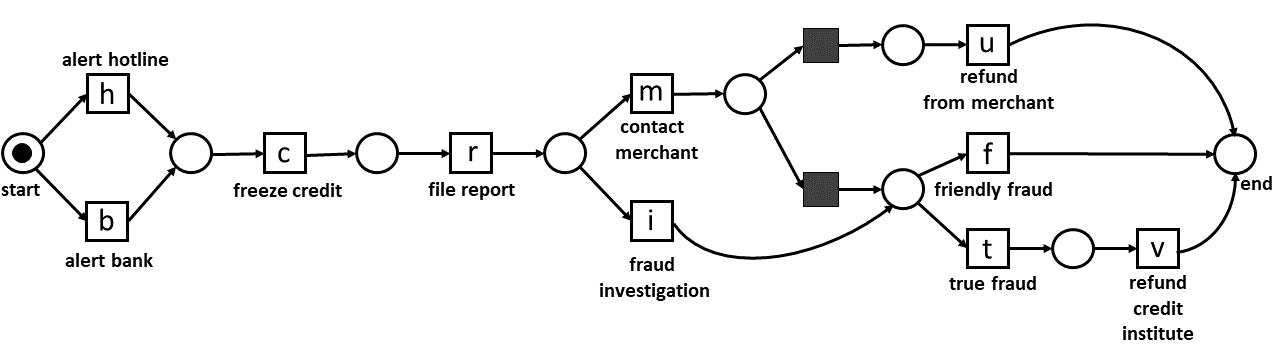
\includegraphics[width=1\columnwidth]{figures/petrinet_cc.png}
	\caption{A petri net visualizing the remote credit card fraud investigation process. This model allows for 10 possible activity traces.}
	\label{fig: petrinet}
	%width=1\columnwidth
\end{figure}

Note that for simplicity, we have used single letters to represent the activity labels in the petri net transitions.
Some possible traces in this process are for example:
$\langle h,c,r,m,u \rangle$,
$\langle b,c,r,m,f \rangle$,
$\langle h,c,r,i,f \rangle$ and
$\langle b,c,r,i,t,v \rangle$.

Suppose that the credit card company wants to do conformance checking to identify deviant process runs.
While some non-conforming cases may indicate that an investigation was not carried out transparently, other frequently reoccurring deviances may indicate that the process model should be updated as it does not reflect the real process anymore.
The company uses conformance checking to become aware of both these aspects.

In the following we will analyze a process instance identifying cardholder with ID 5167 and containing 6 events, some of which are uncertain (shown in Table \ref{table: credit card case}).
%
%
%
\begin{table}[h]
\caption{Example of an uncertain case from the credit card fraud investigation process.}
	%\centering
	\hspace{-1cm}
	\begin{tabular}{ccccc}
		\textbf{Case ID} & \textbf{Event ID} & \textbf{Activity} & \textbf{Timestamp} & \textbf{Type}\\ \hline
	%\multicolumn{1}{c}{\cellcolor{black!30}\textbf{Case ID}} & 
  %\multicolumn{1}{c}{\cellcolor{black!30}\textbf{Event ID}} &
  %\multicolumn{1}{c}{\cellcolor{black!30}\textbf{Timestamp}}
  %\\\hline
	\multicolumn{1}{|c|}{5167} & 
	\multicolumn{1}{|c|}{$e_1$} &
	\multicolumn{1}{|c|}{$h$ (alert hotline)} &
  	\multicolumn{1}{c|}{\begin{tabular}[c]{@{}c@{}} 05-10-2020 23:00
  	\end{tabular}}&
	\multicolumn{1}{|c|}{$!$} 
\\ \hline
	\multicolumn{1}{|c|}{5167} & 
	\multicolumn{1}{|c|}{$e_2$} &
	\multicolumn{1}{|c|}{$c$ (freeze credit)} &
  	\multicolumn{1}{c|}{\begin{tabular}[c]{@{}c@{}} 06-10-2020 \end{tabular}}&
	\multicolumn{1}{|c|}{$!$} 
\\ \hline
	\multicolumn{1}{|c|}{5167} & 
	\multicolumn{1}{|c|}{$e_3$} &
	\multicolumn{1}{|c|}{$r$ (file report)} &
  	\multicolumn{1}{c|}{\begin{tabular}[c]{@{}c@{}} $U$(05-10-2020 20:00, 06-10-2020 10:00) \end{tabular}}&
	\multicolumn{1}{|c|}{$!$} 
\\ \hline
	\multicolumn{1}{|c|}{5167} & 
	\multicolumn{1}{|c|}{$e_4$} &
	\multicolumn{1}{|c|}{$i$ (fraud investigation)} &
  	\multicolumn{1}{c|}{\begin{tabular}[c]{@{}c@{}} 09-10-2020 10:00 \end{tabular}}&
	\multicolumn{1}{|c|}{$!$} 
\\ \hline
	\multicolumn{1}{|c|}{5167} & 
	\multicolumn{1}{|c|}{$e_5$} &
	\multicolumn{1}{|c|}{\shortstack{$\{f: 0.3$ (friendly fraud), \\ $t: 0.7$ (true fraud)$\}$}} &
  	\multicolumn{1}{c|}{\begin{tabular}[c]{@{}c@{}} 14-10-2020 09:00 \end{tabular}}&
	\multicolumn{1}{|c|}{$!$} 
\\ \hline
	\multicolumn{1}{|c|}{5167} & 
	\multicolumn{1}{|c|}{$e_6$} &
	\multicolumn{1}{|c|}{$v$ (refund credit institute)} &
  	\multicolumn{1}{c|}{\begin{tabular}[c]{@{}c@{}} 15-10-2020 10:00 \end{tabular}}&
	\multicolumn{1}{|c|}{$?$} 
\\ \hline
	\end{tabular}
	\label{table: credit card case}
\end{table} 
%
%
%
Suppose that in the first half of October 2020, the company was implementing a new system for automatic event data generation.
During this time, the event data regarding the credit card fraud investigation process often had to be inserted manually from the employees.
Such manual recordings were subject to inaccuracies, leading to imprecise or missing data affecting the cases during this period.
The process instance from Table \ref{table: credit card case} is one of the affected instances.
Here the events $e_2,e_3,e_5,e_6$ are uncertain.
The timestamp of event $e_2$ is not precise enough so the possible timestamp lies between 06-10-2020 00:00 and 07-10-2020 00:00.
Event $e_3$ has happened some time between 20:00 on October 5th and 10:00 on October 6th. 
Event $e_5$ has two possible activity labels: $f$ with probability $0.3$ and $t$ with probability $0.7$.
Refunding the customer (event $e_6$) has been recorded in the system but the customer has not received the money yet, that is why the event is indeterminate.

Figure \ref{fig: beh graph credit card} shows the behavior graph of this event set.
%
%
%
%
\begin{figure}[h] 
\centering

	\begin{tikzpicture}[->,>=stealth',shorten >=1pt,node 						distance=2.5cm,auto,main node/.style={circle,draw,align=center}]
	%\draw [help lines] (0,0) grid (7,2);
	\node[main node,label=above:  {$h$}] (A) at (0,2) {$e_1$};
	\node[main node,label=above: {$c$}] (B) at (2,2) {$e_2$};
	\node[main node,label=above:  {$r$}] (C) at (1,0) {$e_3$};
	\node[main node,label=above:  {$i$}] (D) at (4,1) {$e_4$};
	\node[main node,label=above: {$\{f,t\}$}] (E) at (6,1) {$e_5$};
	\node[main node,dashed,label=above: {$v$}] (F) at (8,1) {$e_6$};
	
	\path
	(A) edge (B)
	(B) edge (D)
	(C) edge (D)
	(D) edge (E)
	(E) edge (F)
	

	;
	\end{tikzpicture}
	\caption{The behavior graph of event set from Table \ref{table: credit card case}. The labels above the nodes indicate the activities executed by each event, the dashed nodes indicate indeterminate events while the graph structure incorporates the uncertainty in timestamps.
	}
	\label{fig: beh graph credit card}
\end{figure}
%
%
%
After computing the valid permutations on set $E=\{e_1,...,e_6\}$, we obtain 
$\mathcal{R}_e$=$\{
\underbrace{\langle e_1,e_2,e_3,e_4,e_5,e_6\rangle}_{s_e^1}$, 
$\underbrace{\langle e_1,e_3,e_2,e_4,e_5,e_6\rangle}_{s_e^2}$,
$\underbrace{\langle e_3,e_1,e_2,e_4,e_5,e_6\rangle}_{s_e^3}$,
$\underbrace{\langle e_1,e_2,e_3,e_4,e_5\rangle}_{s_e^4}$,
$\underbrace{\langle e_1,e_3,e_2,e_4,e_5\rangle}_{s_e^5}$,
$\underbrace{\langle e_3,e_1,e_2,e_4,e_5\rangle}_{s_e^6}
\}$.
Each of these sequences enables two activity traces:
\begin{align*}
A(s_e^1)&= \{ \underbrace{\langle h,c,r,i,f,v \rangle}_{s_a^{1'}}, \underbrace{\langle h,c,r,i,t,v \rangle}_{s_a^{1''}}\} ~,~~
A(s_e^2)= \{ \underbrace{\langle h,r,c,i,f,v \rangle}_{s_a^{2'}}, \underbrace{\langle h,r,c,i,t,v \rangle}_{s_a^{2''}}\}, \\
A(s_e^3)&= \{ \underbrace{\langle r,h,c,i,f,v \rangle}_{s_a^{3'}}, \underbrace{\langle r,h,c,i,t,v \rangle}_{s_a^{3''}}\} ~,~~
A(s_e^4)= \{ \underbrace{\langle h,c,r,i,f \rangle}_{s_a^{4'}}, \underbrace{\langle h,c,r,i,t \rangle}_{s_a^{4''}}\}, \\
A(s_e^5)&= \{ \underbrace{\langle h,r,c,i,f \rangle}_{s_a^{5'}}, \underbrace{\langle h,r,c,i,t \rangle}_{s_a^{5''}}\} ~,~~
A(s_e^6)= \{ \underbrace{\langle r,h,c,i,f \rangle}_{s_a^{6'}}, \underbrace{\langle r,h,c,i,t \rangle}_{s_a^{6''}}\}.
\end{align*}
Note that each activity trace is only enabled by a single event trace.
This is always the case when there are no two events sharing a common activity label.

Each event sequence enables two activity sequences because event $e_5$ has two possible activity labels.
Since for events $e \in E \setminus \{e_5\}$ we have $f_A^e$ equal to 1 for their corresponding unique activity label, the probability that an event sequence $s_e \in \mathcal{R}_e$ has some activity trace $s_a \in A(s_e)$ only depends on whether the trace $s_a$ contains activity $f$ or $t$.
Thus, for traces $s_a^{1'},s_a^{2'},s_a^{3'},s_a^{4'},s_a^{5'},s_a^{6'}$ and their unique enabling sequences we always have $P_a(s_a^{i'} \mid s_e^{i}) = f_A^{e_5}(f) = 0.3$ where $i \in \{1,...,6\}$.
Similarly, for traces $s_a^{1''},s_a^{2''},s_a^{3''},s_a^{4''},s_a^{5''},s_a^{6''}$ and their unique enabling sequences we always have $P_a(s_a^{i''} \mid s_e^{i}) = f_A^{e_5}(t) = 0.7$ where $i \in \{1,...,6\}$.

Next we calculate the $P_e$ values for the 6 possible event sequences in $\mathcal{R}_e$.
First we determine that the uncertain process instance has weak uncertainty in timestamps and strong uncertainty in the event qualifier, so it belongs to the $[T]_{\mathbb{W}}[O]_{\mathbb{S}}$ scenario.
Since there is only one indeterminate event, we have $k = 2$.
The $P_e$-values are displayed in Table \ref{table: Pe values}.

%
%
%
\begin{table}[h]
\caption{The possible event sequences of the process instance from Table \ref{table: credit card case} and their probabilities.}
	\centering
	\begin{tabular}{ccc}
		\textbf{Event sequences} & \textbf{$I(s_e)$} & \textbf{$P_e(s_e)$}
		\\ \hline
	%\multicolumn{1}{c}{\cellcolor{black!30}\textbf{Case ID}} & 
  %\multicolumn{1}{c}{\cellcolor{black!30}\textbf{Event ID}} &
  %\multicolumn{1}{c}{\cellcolor{black!30}\textbf{Timestamp}}
  %\\\hline
	\multicolumn{1}{|c|}{$~ s_e^1:~\langle e_1,e_2,e_3,e_4,e_5,e_6\rangle ~$} & 
	\multicolumn{1}{|c|}{$~ 0.14859 ~$} &
	\multicolumn{1}{|c|}{$~ 0.07429 ~$} 
\\ \hline
	\multicolumn{1}{|c|}{$s_e^2:~\langle e_1,e_3,e_2,e_4,e_5,e_6\rangle$} & 
	\multicolumn{1}{|c|}{$0.77989$} &
	\multicolumn{1}{|c|}{$0.38995$} 
\\ \hline
	\multicolumn{1}{|c|}{$s_e^3:~\langle e_3,e_1,e_2,e_4,e_5,e_6\rangle$} & 
	\multicolumn{1}{|c|}{$0.07151$} &
	\multicolumn{1}{|c|}{$0.03576$} 
\\ \hline
	\multicolumn{1}{|c|}{$s_e^4:~\langle e_1,e_2,e_3,e_4,e_5\rangle$} & 
	\multicolumn{1}{|c|}{$0.14859$} &
	\multicolumn{1}{|c|}{$0.07429$} 
\\ \hline
	\multicolumn{1}{|c|}{$s_e^5:~\langle e_1,e_3,e_2,e_4,e_5\rangle$} & 
	\multicolumn{1}{|c|}{$0.77989$} &
	\multicolumn{1}{|c|}{$0.38995$} 
\\ \hline
	\multicolumn{1}{|c|}{$s_e^6:~\langle e_3,e_1,e_2,e_4,e_5\rangle$} & 
	\multicolumn{1}{|c|}{$0.07151$} &
	\multicolumn{1}{|c|}{$0.03576$} 
\\ \hline
	\end{tabular}
	\label{table: Pe values}
\end{table} 
%
%
%
One can notice that the $I$ values only depend on the ordering of the first three events, which are also the only ones with overlapping timestamps.
Since the indeterminate event $e_6$ does not overlap with any other event, pairs of sequences where the first three events have the same order also have the same probability.
This reflects our assumption that the occurrence and non-occurrance of $e_6$ are both equally possible.
Table \ref{table: p values} displays the calculations for the computation of the $\textbf{p}$ values for all activity traces.
Note that the numbers in both Tables \ref{table: Pe values} and \ref{table: p values} have been rounded.

%
%
%
\begin{table}[h]
	\caption{The set of possible activity traces of the example from Table \ref{table: credit card case}, their enablers, their probabilities and their conformance scores. The conformance score is equal to the cost of the optimal alignment between the trace and the petri net in Fig. \ref{fig: petrinet}. In this example, every activity trace has only one event sequence enabling it.}
	\centering
	\begin{tabular}{cccc}
		\textbf{Activity trace $s_a$} & \textbf{Enablers}($s_a$) & \textbf{$\textbf{p}(s_a)$} & \textbf{$Conf(s_a,M)$}
		\\ \hline
	%\multicolumn{1}{c}{\cellcolor{black!30}\textbf{Case ID}} & 
  %\multicolumn{1}{c}{\cellcolor{black!30}\textbf{Event ID}} &
  %\multicolumn{1}{c}{\cellcolor{black!30}\textbf{Timestamp}}
  %\\\hline
	\multicolumn{1}{|c|}{$~s_a^{1'}: ~ \langle h,c,r,i,f,v \rangle~$} & 
	\multicolumn{1}{|c|}{$~ s_e^1 ~$} & 
	\multicolumn{1}{|c|}{$~ P_e(s_e^1) \cdot P_a(s_a^{1'} \mid s_e^1) = 0.02229 ~$} &
	\multicolumn{1}{|c|}{$~ 1 ~$}
\\ \hline
	\multicolumn{1}{|c|}{$s_a^{1''}: ~ \langle h,c,r,i,t,v \rangle$} & 
	\multicolumn{1}{|c|}{$s_e^1$} & 
	\multicolumn{1}{|c|}{$~ P_e(s_e^1) \cdot P_a(s_a^{1''} \mid s_e^1) = 0.05201 ~$} &
	\multicolumn{1}{|c|}{$~ 0 ~$}
\\ \hline
	\multicolumn{1}{|c|}{$s_a^{2'}: ~ \langle h,r,c,i,f,v\rangle$} & 
	\multicolumn{1}{|c|}{$s_e^2$} & 
	\multicolumn{1}{|c|}{$~ P_e(s_e^2) \cdot P_a(s_a^{2'} \mid s_e^2) =  0.11698~$} &
	\multicolumn{1}{|c|}{$~ 3 ~$}
\\ \hline
	\multicolumn{1}{|c|}{$s_a^{2''}: ~ \langle h,r,c,i,t,v\rangle$} & 
	\multicolumn{1}{|c|}{$s_e^2$} & 
	\multicolumn{1}{|c|}{$~ P_e(s_e^2) \cdot P_a(s_a^{2''} \mid s_e^2) = 0.27296~$} &
	\multicolumn{1}{|c|}{$~ 2 ~$}
\\ \hline
	\multicolumn{1}{|c|}{$s_a^{3'}: ~ \langle r,h,c,i,f,v\rangle$} & 
	\multicolumn{1}{|c|}{$s_e^3$} & 
	\multicolumn{1}{|c|}{$~ P_e(s_e^3) \cdot P_a(s_a^{3'} \mid s_e^3) = 0.01073~$} &
	\multicolumn{1}{|c|}{$~ 3 ~$}
\\ \hline
	\multicolumn{1}{|c|}{$s_a^{3''}: ~ \langle r,h,c,i,t,v\rangle$} & 
	\multicolumn{1}{|c|}{$s_e^3$} & 
	\multicolumn{1}{|c|}{$~ P_e(s_e^3) \cdot P_a(s_a^{3''} \mid s_e^3) = 0.02503~$} &
	\multicolumn{1}{|c|}{$~ 2 ~$}
\\ \hline
\multicolumn{1}{|c|}{$~s_a^{4'}: ~ \langle h,c,r,i,f \rangle~$} & 
	\multicolumn{1}{|c|}{$~ s_e^4 ~$} & 
	\multicolumn{1}{|c|}{$~ P_e(s_e^4) \cdot P_a(s_a^{4'} \mid s_e^4) = 0.02229 ~$} &
	\multicolumn{1}{|c|}{$~ 0 ~$}
\\ \hline
	\multicolumn{1}{|c|}{$s_a^{4''}: ~ \langle h,c,r,i,t \rangle$} & 
	\multicolumn{1}{|c|}{$s_e^4$} & 
	\multicolumn{1}{|c|}{$~ P_e(s_e^4) \cdot P_a(s_a^{4''} \mid s_e^4) = 0.05201~$} &
	\multicolumn{1}{|c|}{$~ 1 ~$}
\\ \hline
	\multicolumn{1}{|c|}{$s_a^{5'}: ~ \langle h,r,c,i,f\rangle$} & 
	\multicolumn{1}{|c|}{$s_e^5$} & 
	\multicolumn{1}{|c|}{$~ P_e(s_e^5) \cdot P_a(s_a^{5'} \mid s_e^5) = 0.11698~$} &
	\multicolumn{1}{|c|}{$~ 2 ~$}
\\ \hline
	\multicolumn{1}{|c|}{$s_a^{5''}: ~ \langle h,r,c,i,t\rangle$} & 
	\multicolumn{1}{|c|}{$s_e^5$} & 
	\multicolumn{1}{|c|}{$~ P_e(s_e^5) \cdot P_a(s_a^{5''} \mid s_e^5) = 0.27296~$} &
	\multicolumn{1}{|c|}{$~ 3 ~$}
\\ \hline
	\multicolumn{1}{|c|}{$s_a^{6'}: ~ \langle r,h,c,i,f\rangle$} & 
	\multicolumn{1}{|c|}{$s_e^6$} & 
	\multicolumn{1}{|c|}{$~ P_e(s_e^6) \cdot P_a(s_a^{6'} \mid s_e^6) = 0.01073~$} &
	\multicolumn{1}{|c|}{$~ 2 ~$}
\\ \hline
	\multicolumn{1}{|c|}{$s_a^{6''}: ~ \langle r,h,c,i,t\rangle$} & 
	\multicolumn{1}{|c|}{$s_e^6$} & 
	\multicolumn{1}{|c|}{$~ P_e(s_e^6) \cdot P_a(s_a^{6''} \mid s_e^6) = 0.02503~$} &
	\multicolumn{1}{|c|}{$~ 3 ~$}
\\ \hline
	\end{tabular}
	\label{table: p values}
\end{table} 
% 
%
%
Now we can compute the expected conformance score for the uncertain process instance with event set $E=\{e_1,...,e_6\}$:
\begin{align*}
Conf(E) &= \sum_{s_a \in \mathcal{R}_a(E)} \textbf{p}(s_a) \cdot conf(s_a,M) \\
&= 0.02229 \cdot 1 + 0.05201 \cdot 0 + 0.11698 \cdot 3 + 0.27296 \cdot 2 \\ 
&+ 0.01073 \cdot 3 + 0.02503 \cdot 2 +
0.02229 \cdot 0 + 0.05201 \cdot 1 \\
&+ 0.11698 \cdot 2 + 0.27296 \cdot 3 + 0.01073 \cdot 2 + 0.02503 \cdot 3 \\
&= 2.2028.
\end{align*}

Given that the information on uncertainty and the assumptions made regarding the independencies within that information are correct, this conformance score is a better estimate of the real conformance score compared to taking the best, worst or average scores with values 0, 3 and 1.75 respectively. 
%Assuming uniform distribution over the above set of activity trace realizations, the weighted conformance score would equate the average conformance score of 1.75.\\


\section{Validation of Probability Estimates}
In this section we compute the probability estimates for the trace realizations of some example process instance and then validate those estimates on two different aspects:
First we show how the expected conformance score of an uncertain trace might be much different than taking the best, worst or average score.
Second, we show that the obtained estimate values are correct by conducting a Monte Carlo simulation on the behavior net of the uncertain trace.
We run the simulation 100000 times and then compare the frequency of each trace realization during the simulation with the probability estimate we computed with our new method.
The experiment has been implemented in Python \textcolor{red}{codelink}.
%
%
%
%
\begin{figure}[h] 
\centering

	\begin{tikzpicture}[->,>=stealth',shorten >=1pt,node 						distance=2.5cm,auto,main node/.style={circle,draw,align=center}]
	%\draw [help lines] (0,0) grid (8,5);
	\node[main node,label=above:  \large{$a$}] (A) at (2,2) {$e_1$};
	\node[main node,label=above: \Large{$\substack{b:~0.9\\ c:~0.1}$}] (B) at (4,3) {$e_2$};
	\node[main node,dashed,label=above: \large{$d$}, label=below:  \Large{$\substack{!:~0.2\\ ?:~0.8}$}] (C) at (4,1) {$e_3$};
	\node[main node,label=above:  \large{$e$}] (D) at (6,2) {$e_4$};

	
	\path
	(A) edge (B)
	(A) edge (C)
	(C) edge (D)
	(B) edge (D)
	

	;
	\end{tikzpicture}
	\caption{The behavior graph of a process instance with strong uncertainty in timestamps and weak uncertainty in activities and event type.
	}
	\label{fig: validation beh graph}
\end{figure}
%
%
%
%
%
%
\begin{table}[h]
	\centering
	\hspace{-1cm}
	\begin{tabular}{cccc}
		\textbf{Trace $s_a$} & \textbf{Enablers}($s_a$) & \textbf{$\textbf{p}(s_a)$} & \textbf{$Conf(s_a,M)$}
		\\ \hline
	%\multicolumn{1}{c}{\cellcolor{black!30}\textbf{Case ID}} & 
  %\multicolumn{1}{c}{\cellcolor{black!30}\textbf{Event ID}} &
  %\multicolumn{1}{c}{\cellcolor{black!30}\textbf{Timestamp}}
  %\\\hline
	\multicolumn{1}{|c|}{$~s_a^{1}: ~ \langle a,b,e \rangle~$} &                                                 	\multicolumn{1}{|c|}{$~s_e^{1}: ~ \langle e_1,e_2,e_4 \rangle~$} & 
	\multicolumn{1}{|c|}{$P_e(s_e^1) \cdot P_a(s_a^1 | s_e^1) 
		=  0.8 \cdot 0.9  = 0.72$}  & 
	\multicolumn{1}{|c|}{$3$} 
\\ \hline  
	\multicolumn{1}{|c|}{$s_a^{2}: ~ \langle a,b,d,e \rangle$} & 
	\multicolumn{1}{|c|}{$s_e^2: \langle e_1,e_2,e_3,e_4 \rangle$} & 
	\multicolumn{1}{|c|}{$~ P_e(s_e^2) \cdot P_a(s_a^2 \mid s_e^2) = (0.5 \cdot 0.2) \cdot 0.9 = 0.09 ~$} &
	\multicolumn{1}{|c|}{$~ 2 ~$}
\\ \hline
	\multicolumn{1}{|c|}{$s_a^{3}: ~ \langle a,d,b,e \rangle$} & 
	\multicolumn{1}{|c|}{$s_e^3: \langle e_1,e_3,e_2,e_4 \rangle$} & 
	\multicolumn{1}{|c|}{$~ P_e(s_e^3) \cdot P_a(s_a^3 \mid s_e^3) =  (0.5 \cdot 0.2) \cdot 0.9 = 0.09 ~$} &
	\multicolumn{1}{|c|}{$~ 2 ~$}
\\ \hline
	\multicolumn{1}{|c|}{$~s_a^{4}: ~ \langle a,c,e \rangle~$} &                                                       	\multicolumn{1}{|c|}{$~s_e^{4}: ~ \langle e_1,e_2,e_4 \rangle~$} & 
	\multicolumn{1}{|c|}{$P_e(s_e^4) \cdot P_a(s_a^4 | s_e^4)
		=0.8 \cdot 0.1 = 0.08$ }  & 
	\multicolumn{1}{|c|}{$1$}  
\\ \hline  
	\multicolumn{1}{|c|}{$s_a^{5}: ~ \langle a,c,d,e \rangle$} & 
	\multicolumn{1}{|c|}{$s_e^5: \langle e_1,e_2,e_3,e_4 \rangle$} & 
	\multicolumn{1}{|c|}{$~ P_e(s_e^5) \cdot P_a(s_a^5 \mid s_e^5) = (0.5 \cdot 0.2) \cdot 0.1 = 0.01~$} &
	\multicolumn{1}{|c|}{$~ 0 ~$}
\\ \hline
	\multicolumn{1}{|c|}{$s_a^{6}: ~ \langle a,d,c,e \rangle$} & 
	\multicolumn{1}{|c|}{$s_e^6: \langle e_1,e_3,e_2,e_4 \rangle$} & 
	\multicolumn{1}{|c|}{$~ P_e(s_e^6) \cdot P_a(s_a^6 \mid s_e^6) = (0.5 \cdot 0.2) \cdot 0.1 = 0.01~$} &
	\multicolumn{1}{|c|}{$~ 0 ~$}
\\ \hline
	\end{tabular}
	\hfill
	\caption{The set of activity trace realizations of the process instance from Figure \ref{fig: validation beh graph}, their enablers, their probabilities and their conformance scores. The conformance score is equal to the cost of the optimal alignment between the trace and the petri net in Fig. \ref{fig: validation model}.}
	\label{table: validation estimates}
\end{table} 
% 
%
%
%

The process instance of our example has strong uncertainty in timestamps and weak uncertainty in activities and event type.
It consists of 4 events: $e_1,e_2,e_3$ and $e_4$, where $e_2$ and $e_3$ have overlapping timestamps.
Event $e_2$ executes $b$ with probability 0.9 and $c$ with probability 0.1.
Event $e_3$ is indeterminate and there is a probability of 0.2 that it did not occurr.
Figure \ref{fig: validation beh graph} shows the corresponding behavior graph.
The first two columns from Table \ref{table: validation estimates} list all the possible activity traces beside the event sequences enabling them.
The third column shows how the probabilities are obtained for each trace realization considering the $[T]_{\mathbb{S}}[A,O]_{\mathbb{W}}$ uncertainty scenario.
In the last column the alignment scores between each possible trace and the model from Figure \ref{fig: validation model} are shown.
Notice how in this specific example, traces that show a worse conformance score are the most likely ones, while the conforming traces are very unlikely in comparison.
The uncertain trace in the example has an expected conformance score of 2.6.
Assuming uniform distribution over the trace realizations would yield a more optimistic expected conformance score of approximately 1.33, while taking the best conformance score 0 would be even further from our computed score.
%
%
%
\begin{figure}
	\centering
	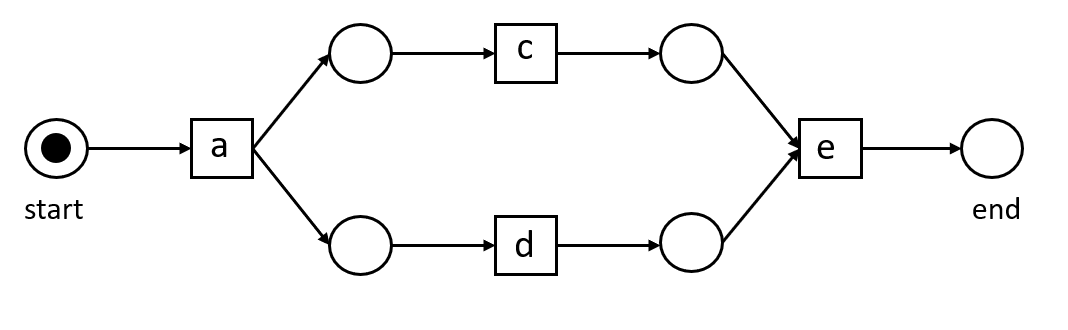
\includegraphics[width=0.8\columnwidth]{figures/model_validation.png}
	\caption{A petri net visualizing the normative model of the process during which the instance from Table \ref{table: validation estimates} was executed.}
	\label{fig: validation model}
	%width=1\columnwidth
\end{figure}
%
%
%
%
%
%
\begin{figure}
	\centering
	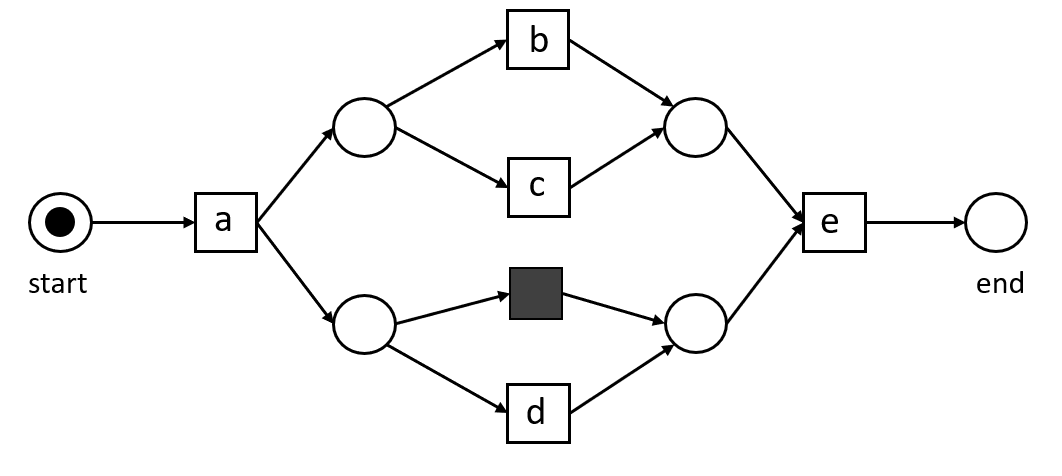
\includegraphics[width=0.8\columnwidth]{figures/behaviornet.png}
	\caption{The behavior net obtained from the behavior graph in Figure \ref{fig: validation beh graph}.}
	\label{fig: behavior net}
	%width=1\columnwidth
\end{figure}
%
%
%
%
%
%
For the same process instance from Figure \ref{fig: validation beh graph}, we now validate our obtained probability estimates quantitatively by means of the Monte Carlo simulation approach.
First we construct the behavior net corresponding to the uncertain process instance which is shown in Figure \ref{fig: behavior net}.
The set of replayable traces in this behavior net is exactly the set of activity trace realizations for the uncertain instance.
Then we run a simulator on the behavior net 100000 times producing 100000 possible traces.
After each run, we divide the accumulated count of each trace variant by the number of runs, and compare those values to our probability estimates.
The simulator we use here is provided in the PM4Py library and it is called a stochastic simulator.
The stochastic simulator picks in every step of the simulation one transition out of the set of enabled transitions according to a stochastic map, assigning a weight to each transition in the petri net (here: behavior net). 
The next transition to fire is picked randomly following a probability distribution over the set of enabled transitions. 
If not specified otherwise, each transition $t$ initially has $weight(t)=1$ in the stochastic map. 
In each step, a new probability distribution is computed over the set of enabled transitions by dividing their weight with the sum of the weights of the enabled transitions (normalization). 
By default, this distribution is always uniform. 
One can also assign specific weights to the transitions. 
These weights become relevant by (potentially) leading to non-uniform distributions when the simulator randomly picks the next transition to fire. 
There are two scenarios on when the weights affect the random choice the simulator: 
\begin{itemize}
\item The XOR-split:
The transitions in an XOR-split pairwise exclude each-other. 
How often each of them is chosen will roughly reflect how their weights compare to each-other.
\item The AND-split:
All paths following the AND-split will certainly be taken by the simulator. 
\end{itemize}
Since the weights are only defined for transitions and not explicitly for arcs in the petri net, which path is taken first (or second and so on) depends on the probability distribution over all enabled transitions at that moment. 
The probability of one particular path being taken (meaning one of its transitions is fired) is then equal to the sum of the weights of the transitions that are enabled following that particular path over the sum of the weights of all enabled transitions over all paths in the AND-split.\\
To simulate our uncertainties in activities, events and timestamps we do the following: 
Possible activities executed by the same event appearing in an XOR-split in the behavior net get weights so that in relation to each-other their weights reflect how much more likely one activity is compared to the other one(s). 
Whether an event with a unique activity is executed or not (uncertainty in event type), is equivalently modeled as an XOR-choice between a visible transition and a silent one in the behavior net (see Def. \ref{def: bn}). 
If there are two or more possible acitivities for an indeterminate event, then the sum of the weights of the visible transitions in relation to the weight of the silent transition should be the same as in the distribution given in the event type uncertainty information.
Regarding timestamps, through the simulator we can only simulate strong uncertainty, that is, uniform distribution over the possible event orderings. Whenever there are events with overlapping timestamps, these appear in an AND-split in the behavior net. 
Which path of the AND-split is taken first (out of the ones that are enabled) signals which event is executed at that moment.
Since one event might have many possible activities and thus transitions, to simulate a uniform distrubution over the choice of the path at any moment, the sum of transitions' weights enabled immediately after following each path should sum up to 1.

In our example behavior net, we assign weights $0.9$, $0.1$, $0.2$ and $0.8$ to transitions $b$, $c$, $d$ and $\tau$ (the silent transition) respectively.
In the beginning, only $a$ can fire.
Afterwards, $b$, $c$, $d$ or $\tau$ are picked, each being assigned probability $weight(\cdot)/ (0.9+0.1+0.8+0.2)$, yielding a probability distribution over the enabled transitions assigning weights $0.45,0.05,0.4,0.1$ to $b$, $c$, $d$ and $\tau$ respectively. 
Executing $b$ is still $0.9/0.1=0.45/0.05=9$ times more likely than executing $c$ and thus reflecting the weak uncertainty in activities, whereas executing $d$ is still $0.2/0.8=0.1/0.4=1/4$ times less likely than skipping it and thus reflecting the weak uncertainty in the event type.
In the simulation, there is always the choice of whether the upper path is taken first ($b$ or $c$ fires first), or whether the lower path is taken (executing $d$ or skipping it). 
This decision is made when all four transitions: $b$, $c$, $d$ and $\tau$ make up the set of enabled transitions. 
For example, the probability of executing $b$ will be:
$weight(b)/(weight(b)+weight(c)+weight(d)+weight(\tau))$. 
Since taking the upper path first implies $e_2$ happening before $e_3$ whereas the lower path implies $e_3$ happening before $e_2$, and we have no information on which is more likely, we want each of those paths to be taken equally often. 
This is possible whenever $weight(b) + weight(c)=weight(d)+weight(\tau)$. 
By construction, whenever those three transitions are enabled, in roughly half the cases $b$ or $c$ will be executed first, and in the other half $d$ or $\tau$.
If $b$ or $c$ happens first, then executing $d$ in the next step will have probability 0.2/(0.8+0.2) = 0.2. 
If $d$ or $\tau$ fires first, then the enabled transitions will be $b$ and $c$, where $b$ will get probability 0.9 and $c$ 0.1.

Applying the stochastic simulator $n$ times on the the behavior net where the transitions have the particular weights we explained above, yields $n$ traces.
For each possible trace out of the 6 trace realizations for the uncertain process instance, dividing the frequency of that trace by $n$ yields a probability estimate for that trace.
As expected, Figures \ref{fig: abe}-\ref{fig: adce} show how for greater $n$, this estimate converges to the probability estimate we computed with our equations in Table \ref{table: validation estimates}.
While we run the simulator for 100000 rounds to obtain more reliable values, we also plot the results for $n$ going from 1 to 1000 runs, to show how the fluctuations of the probabilities decrease and converge to the expected value when $n$ increases.

\begin{figure}%
    \centering
    {{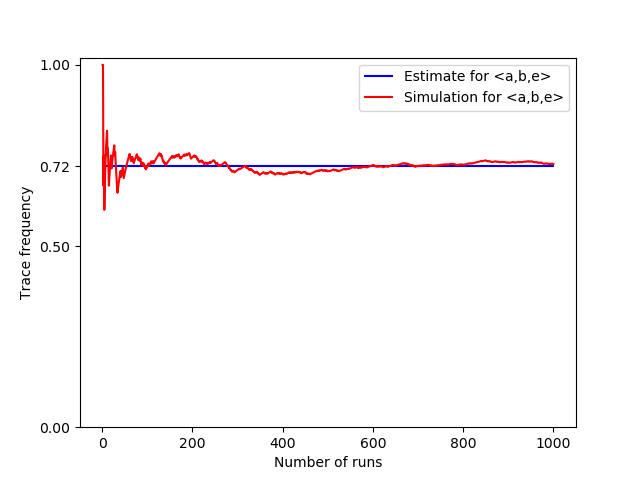
\includegraphics[width=10cm]{figures/abe1.png} }}%
    \qquad
   {{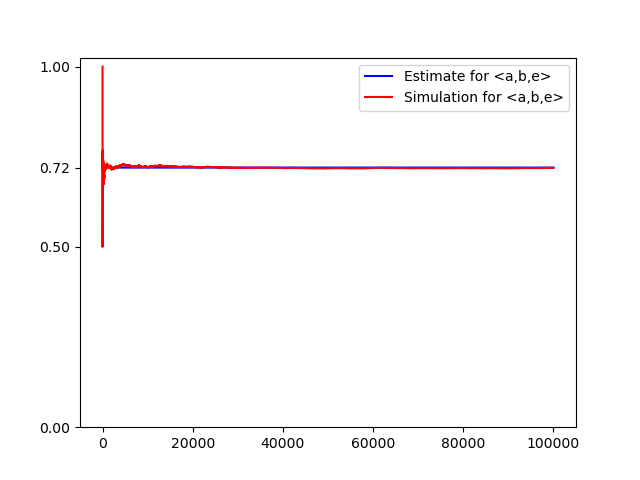
\includegraphics[width=10cm]{figures/abe100.png} }}%
    \caption{Two plots showing how the frequency of trace $\langle a,b,e \rangle$ converges to the expected value of $0.72$ over 1000 runs in the first plot, and 100000 runs in the second plot.}%
    \label{fig: abe}%
\end{figure}
%
%
%
%
%
%
%
\begin{figure}%
    \centering
    {{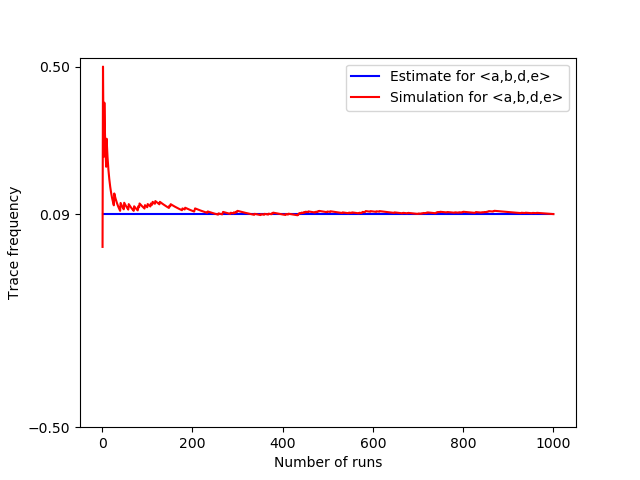
\includegraphics[width=10cm]{figures/abde1.png} }}%
    \qquad
    {{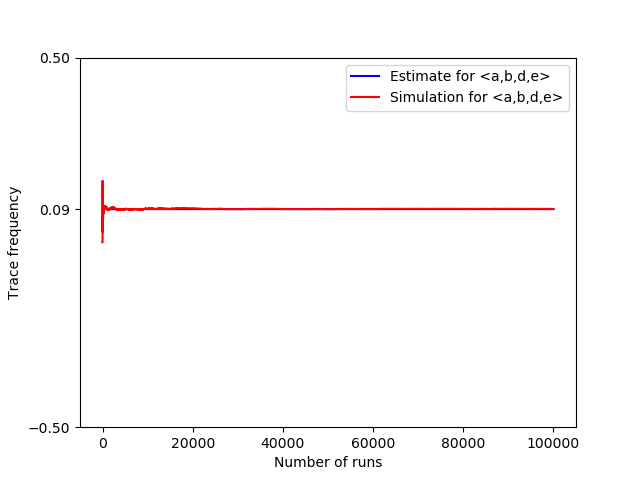
\includegraphics[width=10cm]{figures/abde100.png} }}%
    \caption{Two plots showing how the frequency of trace $\langle a,b,d,e \rangle$ converges to the expected value of $0.09$ over 1000 runs in the first plot, and 100000 runs in the second plot.}%
    \label{fig: abde}%
\end{figure}
%
%
%
%
%
%
\begin{figure}%
    \centering
    {{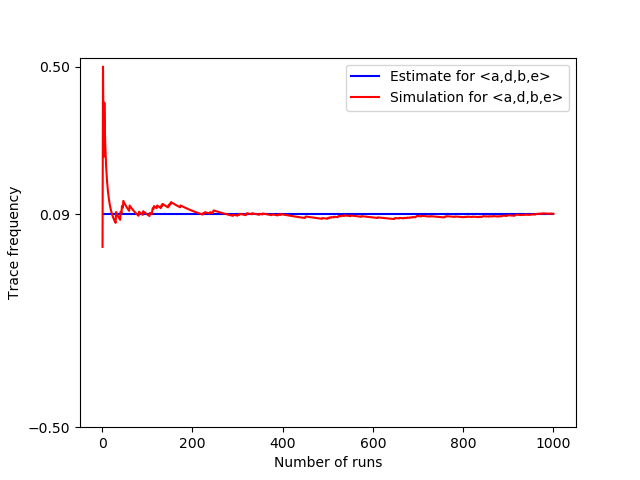
\includegraphics[width=10cm]{figures/adbe1.png} }}%
    \qquad
    {{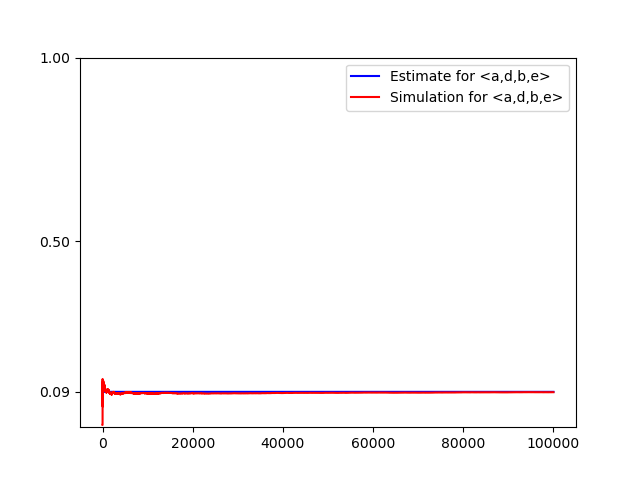
\includegraphics[width=10cm]{figures/adbe100.png} }}%
    \caption{Two plots showing how the frequency of trace $\langle a,d,b,e \rangle$ converges to the expected value of $0.09$ over 1000 runs in the first plot, and 100000 runs in the second plot.}%
    \label{fig: adbe}%
\end{figure}
%
%
%
%
%
%
\begin{figure}%
    \centering
    {{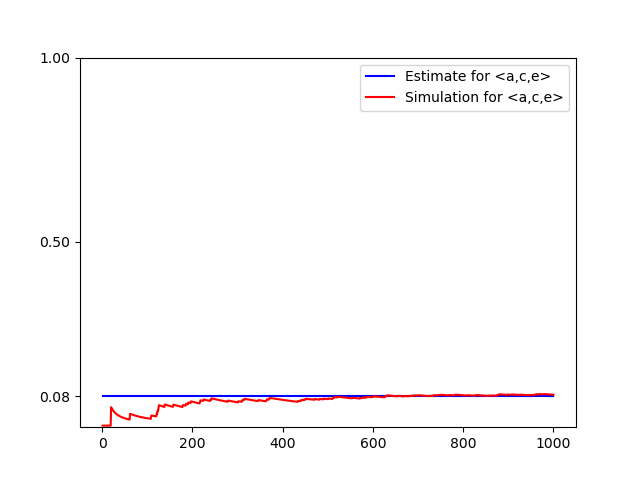
\includegraphics[width=10cm]{figures/ace1.png} }}%
    \qquad
    {{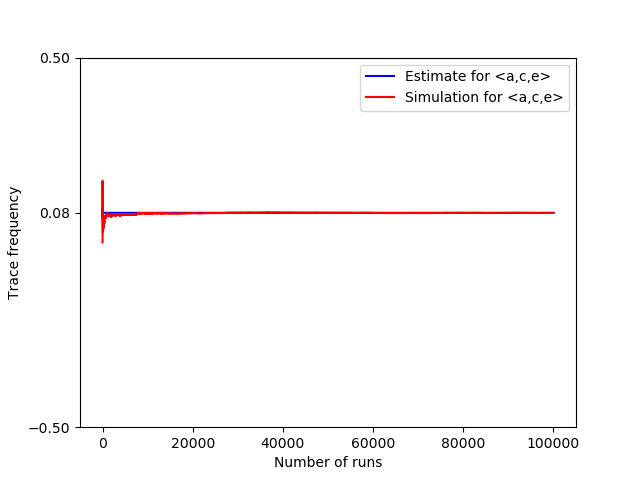
\includegraphics[width=10cm]{figures/ace100.png} }}%
    \caption{Two plots showing how the frequency of trace $\langle a,c,e \rangle$ converges to the expected value of $0.08$ over 1000 runs in the first plot, and 100000 runs in the second plot.}%
    \label{fig: ace}%
\end{figure}
%
%
%
%
%
%
\begin{figure}%
    \centering
    {{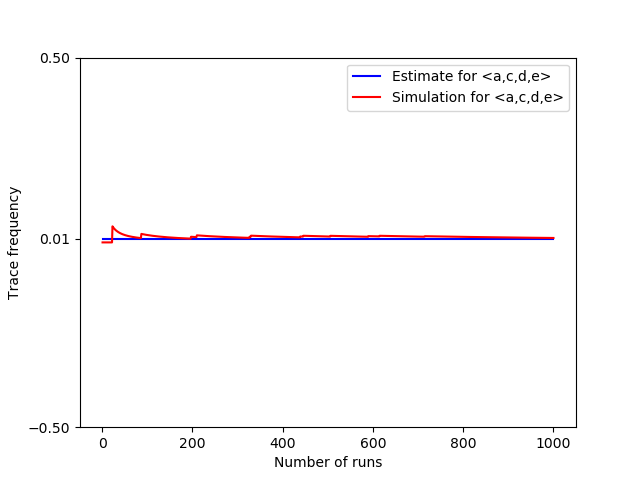
\includegraphics[width=10cm]{figures/acde1.png} }}%
    \qquad
    {{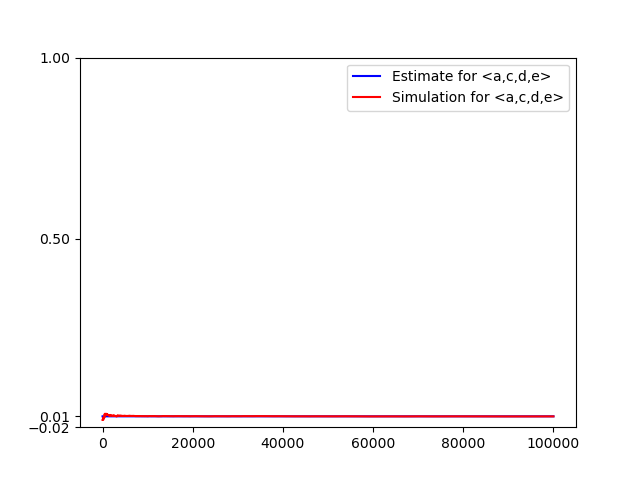
\includegraphics[width=10cm]{figures/acde100.png} }}%
    \caption{Two plots showing how the frequency of trace $\langle a,c,d,e \rangle$ converges to the expected value of $0.01$ over 1000 runs in the first plot, and 100000 runs in the second plot.}%
    \label{fig: acde}%
\end{figure}
%
%
%
%
%
%
\begin{figure}%
    \centering
    {{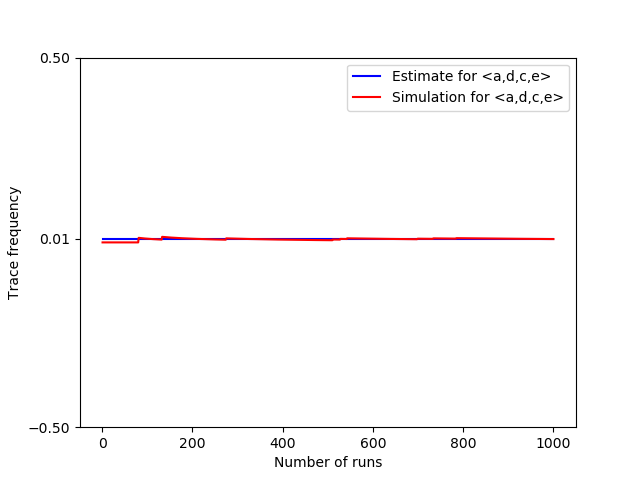
\includegraphics[width=10cm]{figures/adce1.png} }}%
    \qquad
    {{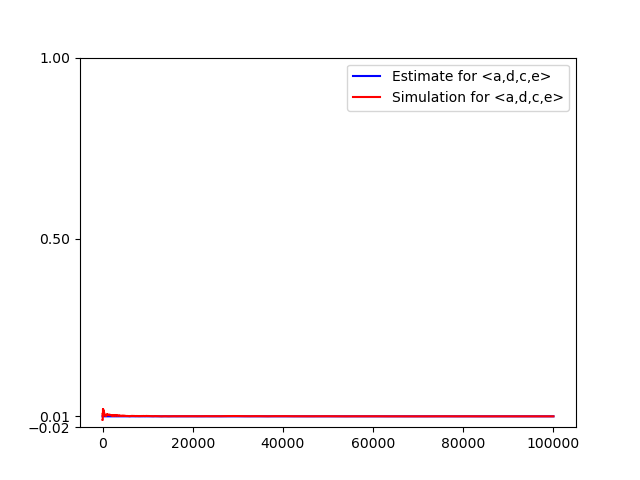
\includegraphics[width=10cm]{figures/adce100.png} }}%
    \caption{Two plots showing how the frequency of trace $\langle a,d,c,e \rangle$ converges to the expected value of $0.01$ over 1000 runs in the first plot, and 100000 runs in the second plot.}%
    \label{fig: adce}%
\end{figure}
%
%
%
%
%
%In the next section we try to improve our probability estimates and therefore the expected conformance score for each uncertain process instance.
%We assume that some trace realization is more likely if there are other traces in the log which are identical or similar to it.
To conclude, the Monte Carlo simulation showed that our estimated probabilities for the trace realizations match their relative frequencies when one simulates the behavior net of the corresponding uncertain process instance.

%
%
%
%
%
%
\newpage
\section{Estimating New Probabilities Using Trace Patterns in Log }
In this section we obtain probability estimates for the trace realizations of uncertain instances by using the information that the rest of the traces from the log provide.
In contrast to the way we obtained these estimates in the last section, the information we exploit here is not the one encoded within each event describing uncertainty explicitly. 
Instead, the new estimate solely quantifies how likely it is to see other traces in the log that are identical or display similar patterns to the current one.
The idea and the proposed models in this section are inspired from the work done in \cite{por}.
The main motivation in \cite{por} is obtaining better conformance assessments for process instances whose events can only be partially ordered.
This happens when the recorded timestamps of some events do not allow a unique (total) order between them.
Possible causes could be lack of synchronization, manual recordings and so on.
In their work, the authors define such events as \textit{uncertain events} and the lack of a  total order on them as \textit{order uncertainty}.

An important assumption affecting the methods used in \cite{por} is that any two events which can not be totally ordered have identical timestamps.
This enables partitioning any event set $E$ belonging to some proces instance from the log into non-empty subsets $E=\langle E_1,...,E_m \rangle $ such that:
\begin{itemize}
\item \textbf{(1)} Any pair of events from different subsets can be totally ordered.
More precisely, for all $1 \leq i < j \leq m$: each event in $E_i$ happened before each event from $E_j$.  
\item \textbf{(2)} All events in the same subset have identical timestamps and therefore every permutation on them is a possible ordering.
\end{itemize}
Certain traces correspond to the special case where $|E_i| = 1$ for all $1 \leq i \leq m$.

Since our definition of uncertainty is broader, the assumption above does not necesarily hold for all uncertain cases.
Given some event set $E$, we can define the subsets of $E$ to be the subsets of vertices in the connected components $(CC(\mathcal{I}))$ of the interval graph $\mathcal{I}(E)$.
By Theorem \ref{theorem: partitioning} we know that all pairs of elements across subsets can be totally ordered and we can sort the events in the components into a sequence $\langle E_1,...,E_{|CC(I)|}\rangle$ in such a way that they satisfy condition \textbf{(1)}.
Condition \textbf{(2)} on the other hand holds if and only if all the connected components in the interval graph induce cliques (see Proposition \ref{prop: clique}).
This is however not always the case.

In the following we adapt the methods introduced in \cite{por} to obtain new probability estimates for the trace realizations based on behavioral regularities in the log.
There are three different approaches, each an estimator incorporating different notions of behavioral abstraction.
In other words, each method gives a different view on what patterns to look for in the other traces from the log in order to measure the likelihood of a particular activity trace realization.
Given a particular activity trace, the level of abstraction of the chosen method determines how similar other traces in the log have to be in order to consider the similarity meaningful and take it into account when measuring the likelihood of the trace.

From now on, suppose that we are given a log $L$ and let $\mathcal{U}_C^L$ be the set of all caseIDs appearing in $L$.
For any $c \in \mathcal{U}_C^L$, let $E_c \subseteq L$ be the maximal set of events belonging to case $c$.
%We define $CertainCases := \{c \in \mathcal{U}_C(L) \mid 
%\forall e \in E_c: e \in \mathcal{E}_C\}$
%to be the set of certain cases, that is those cases whose events are all certain.
%The set of uncertain cases is defined as
%$UncertainCases := \mathcal{U}_C(L) \setminus CertainCases$.
For every case $c \in \mathcal{U}_C^L$ and its event set $E_c$, let $\mathcal{F}(E_c)$ be its follows graph and $\mathcal{I}(E_c)$ be its interval graph.
By sorting the connected components of the interval graph as we explained above, we can always partition $E_c$ into non-empty subsets and order them into a sequence $\langle E_1,...,E_m\rangle$ with $m=|CC(\mathcal{I})|$ such that they satisfy condition \textbf{(1)}.
We use $\lambda(E_c)$ to identify the ordered partition of event set $E_c$.
Note that if one can totally order the events from $E_c$, the subsets in the ordered partitions each have size 1.
Events might be totally ordered by definition of $\prec_{\mathcal{E}}$ even if some of them have uncertain timestamps as long as they do not overlap.
%Additionally, for any certain case $c \in CertainCases$, we use $\sigma_e(c)$ and $\sigma_a(c)$ to identify its unique event and activity trace respectively.


\subsection{Trace equivalence model}
The \textit{trace equivalence model} estimates the probability of a sequence of activities by exploring how often the particular trace is the only possile activity trace of cases with a unique event sequence.
Given some possible activity trace $s_a$ of an uncertain case, we measure its probability as:
\begin{align*}
\textbf{p}_{trace}(s_a) = \eta \cdot \frac{|\{ c \in \mathcal{U}_C^L \mid \mathcal{R}_e(E_c)= \{s_e\} ~ \wedge A(s_e)= \{s_a \} \} }
{|\{ c \in \mathcal{U}_C^L \mid \mathcal{R}_e(E_c)= \{s_e\} ~ \wedge ~ |A(s_e)| = 1\}|}
\end{align*}
where $\eta$ is the normalizing factor over all activity traces of the uncertain case.\\
This way, the probability value that $P_{trace}$ assigns to an activity trace yields the fraction of traces with totally ordered event set and no uncertainty in activities that are equivalent to it.
In contrast to the model definition in \cite{por}, we do not only look at traces containing only certain events, but also include instances with uncertainty in timestamps as long as their event set can still be totally ordered.
While this model is rather simple, it may have limited applicability if there are very few such traces present in the log.
Because of the low abstraction level, it might also be that one can hardly find equivalent traces even if the number in the denominator is large.


\subsection{N-gram model}
Instead of considering only fully equivalent traces, in this model the authors in \cite{por} explore how often subsequences appear in the log.
Given an activity trace, first it is measured how probable it is for each activity in the trace to appear at the corresponding position.
Here the authors measure how often each activity label in the trace succeeds its up to the last $N-1$ preceeding activities.
This estimation is however only based on all traces of the log that contain the relevant activities in the subsequence without order uncertainty.
For this, a predicate $certain$ is defined the following way: 
Given an event set $E$ with $\lambda(E)=\langle E_1,...,E_m\rangle$ and a subsequence $\langle a_1,...,a_l\rangle$ of a possible activity trace $s_a$, we define
\begin{align*}
certain(\langle a_1,...,a_l \rangle, \langle E_1,...,E_m \rangle) \Leftrightarrow \\
\exists ~ i \in \{0,...,m-l\} ~ s.t.~
\forall ~ j \in \{1,...,l\}: E_{i+j} = \{e\} \text{ for some } e \in E \\ \wedge ~ \pi_o(e)=! \wedge ~ \pi_a(e)= a_j.
\end{align*}
This way, a subsequence of activities is considered as \textit{certain} in an event set if there is a subsequence of determinate events which can be certainly ordered in time that execute the activities in the given order.
In contrast to the definition used in \cite{por}, here we also require the events in the subsequence to be determinate.
The predicate helps measure the probability of a particular activity label succeeding its predecessors:
\begin{align*}
P(a ~ | ~ \langle a_1,...,a_l \rangle) = \frac{|\{c \in \mathcal{U}_C^L \mid
certain(\langle a_1,...,a_l,a \rangle, \lambda(E_c)) \}|}
{|\{c \in \mathcal{U}_C^L \mid
certain(\langle a_1,...,a_l \rangle, \lambda(E_c)) \}|}.
\end{align*}
Given a possible activity trace $s_a=\langle a_1,...,a_n\rangle$, its probability is obtained by aggregating the probability of each label suceeding its up to $N-1$ preceding activities in $s_a$:
\begin{align*}
\textbf{p}_{N-gram}(\langle a_1,...,a_n \rangle) =  \eta \cdot
\prod_{k=2}^n P(a_k ~ | ~ \langle a_{max(1,k-N+1)},..., a_{k-1}\rangle)
\end{align*}
where $\eta$ is the normalizing factor over all activity traces of the uncertain case.\\
As explained in \cite{por}, the approach may be adapted to explicitly consider the first events of traces in the assessment by adding a new artificial activity label to the first position of all activity traces in the log.
The authors argue that this model is more abstract compared to the trace equivalence model.
Indeed, it only requires finding existing traces in the log that have equivalent subsequences without uncertainty, instead of fully equivalent certain traces.
This is useful if the process has local dependencies which are independent from other parts of the execution.
Think of a process where the first three activities are always executed in the same order.
Given two activity trace realizations which only differ in the ordering of these first three activities, one might want to consider the trace in which those first three activities have the expected order more likely, even if the rest of both traces find no resemblance in the log.

A drawback is however that in the N-gram model, the behavioral regularities needed to support an uncertain trace always have the form of consecutive activities.
There could be activities whose dependency lies in the fact that they happen in a particular order, but not necessarily consecutively.
This is the motivation behind the third model which we introduce next.



\subsection{Weak Order model}
The \textit{weak order model} proposed in \cite{por} takes all order dependencies into account, even if they do not materialize in the form of consecutive activity executions.
Such activities have an indirect order dependency, a \textit{weak order} from which the method gets its name.
First, a predicate $order$ is defined.
Given two activity labels $a,a'$ and the event set of a process instance from the log, we have:
\begin{align*}
order(a,a',E) \Leftrightarrow 
\exists ~e, e' \in E: ~ e \prec_{\mathcal{E}} e' ~ \wedge \pi_o(e)=! ~ \wedge \pi_o(e')=! \\
\wedge ~ \pi_a(e)=a \wedge \pi_a(e')=a'.
\end{align*}

$Order$
captures whether two particular (and not necessarily distinct) activities appear in a particular order in a given process instance.
Regardless of whether the case in question is certain or uncertain, the predicate is satisfied if there exist two (determinate) events that can be totally ordered in time where the first event executes the first activity and the second one the second activity.
Again, in contrast to the definition used in \cite{por}, here we also require the pair of events to be determinate.
Note that equivalent to verifying whether the events satisfy the $\prec_{\mathcal{E}}$ relation, one could test if there is an arc between them in the follows graph $\mathcal{F}(E)$ (Def. \ref{def: follows graph}).
The predicate helps assessing how often events execute a pair of particular activities in a given order when considering only the traces that certainly contain both activities:
\begin{align*}
P(a,a')= \frac{|\{c \in \mathcal{U}_C^L \mid oder(a,a',E_c)\}|}
{|\{c \in \mathcal{U}_C^L \mid \exists ~ e,e' \in E_c: ~
\pi_a(e)=a \wedge \pi_a(e')=a'\}|}.
\end{align*}
From here on, one estimates the probability of a possible activity trace $s_a=\langle a_1,...,a_n \rangle$ by aggregating the probabilities that each pair of activities in $s_a$ has the order indicated in $s_a$:
\begin{align*}
\textbf{p}_{WO}(\langle a_1,...,a_n \rangle) = \eta \cdot \prod_{
\substack{1 \leq i < n \\ i < j \leq n}}
P(a_i,a_j)
\end{align*}
where $\eta$ is the normalizing factor over all activity traces of the uncertain case.
The weak order model uses the most abstract notion of behavioral regularities when deciding which similarities across traces are considered relevant.

Given an uncertain process instance with event set $E$ and set $\mathcal{R}_a$ containing all possible activity traces, we can compute a new expected conformance score the following way:
\begin{align*}
Conf(E) = \sum_{s_a \in \mathcal{R}_a} \textbf{p}_m(s_a) \cdot conf(s_a,M)
\end{align*}
where $M$ is the process model, $conf(s_a,M)$ yields the conformance score of trace $s_a$ and model $M$ and $m \in \{trace, N$-$gram, WO\}$ is the chosen method.

It is important to stress that in all three methods, the process model itself is not included when evaluating the probabilities.
This is crucial if the probability estimates are used as weights to compute conformance checking scores.
Otherwise, the model would introduce a bias in the conformance checking results, by for example increasing the weights of the conforming traces.

\section{Conformance Checking Combining Two Probability Distributions}
Until now, we have seen how for a given trace realization of an uncertain case we can obtain two probability values: one computed using the information on uncertainty on the event level and one reflecting how similar the trace is to other traces in the log.
Naturally, we can exploit both estimates to aggregate a new probability for each trace.
This is however useful only when the two estimates are computed based on independent information.
This way the information on uncertainty enclosing the events of the uncertain case should not contain information reflecting the model or the behavioral regularities in the log.
Similarly, the probability estimate computed with the trace equivalence model, N-gram or the weak order model should rely only on patterns which appear without uncertainty.
As we saw in the definitions of the three models, uncertain trace realizations are also considered for estimating the probabilities based on trace patterns in the log.
However, such traces display the relevant pattern or behavioral regularity without uncertainty.
 
Assuming that the two probability estimates are independent, a new probability estimate for an activity trace $s_a$ is obtained the following way:
\begin{align*}
&\textbf{p}_{log}(s_a) \gets \textbf{p}_m(s_a) \text{ \hspace*{2cm} where } m \in \{trace,N \text{-}gram,WO\}, \\
&\textbf{p}_{unc}(s_a) \gets \textbf{p}(s_a) \text{\hspace*{2,3cm} as defined in Chapter \ref{chap:estimates}, and} \\ 
&\textbf{p}_{combi}(s_a) = w_{log} \cdot \textbf{p}_{log}(s_a) + w_{unc} \cdot \textbf{p}_{unc}(s_a),
\end{align*}
where $w_{log}, w_{unc}$ are two non-negative weights that sum up to 1.

The values of the weights $w_{log}$ and $w_{unc}$ can be chosen in a way that they reflect the desired focus or our reliability in the estimates and in the data.

%\textcolor{red}{Add small example with artificial log and use Pwo because it is simple but still abstract enough for a small example.}

\subsection{Obtaining Probability Estimates for Example Log}
Suppose we have an uncertain log $L$ containing 35 process instances, from which 29 are certain traces and 6 are uncertain.
We represent $L$ as a multiset of behavior graphs \cite{space} (see fig. \ref{fig: combi estimates}) consisting of 6 distinct graphs.
The first three graphs show the three variants of the 29 certain traces.
Notice that these graphs are paths, there is no uncertainty in activities and all events are determinate.
The other three graphs are the behavior graphs of the 6 uncertain traces.
Suppose that the trace for which we want to estimate the probabilities is the one represented by the last graph having uncertainty type $[A]_{\mathbb{W}}[T]_{\mathbb{S}}$.
Since the two events in the middle can appear in any order, there are two possible event sequences each with probability $1/2$.
Since one of the events in the middle has two possible activity labels, this process instance has four possible activity traces:
$\langle a,b,d,e\rangle, \langle a,c,d,e\rangle, \langle a,d,b,e\rangle$ and $\langle a,d,c,e\rangle$.
As we can see in Table \ref{table: combi traces}, the probability $\textbf{p}_{unc}$ of each activity trace depends on whether the trace contains activity $b$ or activity $c$.
Next we estimate the values of $\textbf{p}_{log}$ for these four traces using the weak order model.
This requires estimating the probability $P(a_1,a_2)$ for all activity pairs $a_1,a_2$ that appear in one of the four traces in this particular order.
These estimates can be obtained from Table \ref{table: combi pairs}.
These values are then aggregated to obtain the weak-order probability values as shown in the third colmun of Table \ref{table: combi pairs}.
%
%
%
%
%
\begin{figure}[h]
	\centering
	\begin{tikzpicture}[->,>=stealth',shorten >=1pt,node 						distance=2.5cm,auto,main node/.style={circle,draw,align=center}]
	%\draw [help lines] (0,0) grid (10,15);
	
	%Graph with #12
	\node[] at (0,15) {\large 12x};
	\node[main node,label=above: \large $a$] (A1) at (1,15) {\textcolor{white}{$e$}};
	\node[main node,label=above: \large $b$] (B1) at (3,15) {\textcolor{white}{$e$}};
	\node[main node,label=above: \large $c$] (C1) at (5,15) {\textcolor{white}{$e$}};
	\node[main node,label=above: \large $d$] (D1) at (7,15) {\textcolor{white}{$e$}};
	\node[main node,label=above: \large $e$] (E1) at (9,15) {\textcolor{white}{$e$}};
	
	%Graph with #10
	\node[] at (0,13) {\large 10x};
	\node[main node,label=above: \large $a$] (A2) at (2,13) {\textcolor{white}{$e$}};
	\node[main node,label=above: \large $b$] (B2) at (4,13) {\textcolor{white}{$e$}};
	\node[main node,label=above: \large $c$] (C2) at (6,13) {\textcolor{white}{$e$}};
	\node[main node,label=above: \large $e$] (D2) at (8,13) {\textcolor{white}{$e$}};

	%Graph with #7
	\node[] at (0,11) {\large 7x};
	\node[main node,label=above: \large $a$] (A3) at (2,11) {\textcolor{white}{$e$}};
	\node[main node,label=above: \large $d$] (B3) at (4,11) {\textcolor{white}{$e$}};
	\node[main node,label=above: \large $c$] (C3) at (6,11) {\textcolor{white}{$e$}};
	\node[main node,label=above: \large $e$] (D3) at (8,11) {\textcolor{white}{$e$}};

	%Graph with #1
	\node[] at (0,9) {\large 1x};
	\node[main node,label=above: \large $a$] (A4) at (1,9) {\textcolor{white}{$e$}};
	\node[main node,label=above: \large $b$] (B4) at (3,9) {\textcolor{white}{$e$}};
	\node[main node,label=above: \large ${\{c,d\}}$] (C4) at (5,9) {\textcolor{white}{$e$}};
	\node[main node,label=above: \large $d$] (D4) at (7,9) {\textcolor{white}{$e$}};
	\node[main node,label=above: \large $e$] (E4) at (9,9) {\textcolor{white}{$e$}};
	
	%Graph with #3
	\node[] at (0,6) {\large 3x};
	\node[main node,label=above: \large $a$] (A5) at (2,6) {\textcolor{white}{$e$}};
	\node[main node,label=above: \large $b$] (B5) at (4,6) {\textcolor{white}{$e$}};
	\node[main node,label=above: \large $c$] (C5) at (6,7) {\textcolor{white}{$e$}};
	\node[main node,label=above: \large $d$] (D5) at (6,5) {\textcolor{white}{$e$}};
	\node[main node,label=above: \large $e$] (E5) at (8,6) {\textcolor{white}{$e$}};	
	
	%Graph to estimate
	\node[] at (0,2) {\large 1x};
	\node[main node,label=above: \large $a$] (A6) at (3,2) {\textcolor{white}{$e$}};
	\node[main node,label=above: \large ${\{b: 0.3, ~c: 0.7\}}$] (B6) at (5,3) {\textcolor{white}{$e$}};
	\node[main node,label=above: \large $d$] (C6) at (5,1) {\textcolor{white}{$e$}};
	\node[main node,label=above: \large $e$] (D6) at (7,2) {\textcolor{white}{$e$}};

	
	\path
	
	(A1) edge (B1)
	(B1) edge (C1)
	(C1) edge (D1)
	(D1) edge (E1)
	
	(A2) edge (B2)
	(B2) edge (C2)
	(C2) edge (D2)
	
	(A3) edge (B3)
	(B3) edge (C3)
	(C3) edge (D3)
	
	(A4) edge (B4)
	(B4) edge (C4)
	(C4) edge (D4)
	(D4) edge (E4)
	
	(A5) edge (B5)
	(B5) edge (C5)
	(B5) edge (D5)
	(C5) edge (E5)
	(D5) edge (E5)
	
	(A6) edge (B6)
	(A6) edge (C6)
	(B6) edge (D6)
	(C6) edge (D6)
	
	%\node[main node,label=above: \large $a$] (A2) at (2,14) {};
	

	;
	\end{tikzpicture}
	\caption{A multiset of 34 behavior graphs representing the traces from an uncertain event log.}
	\label{fig: combi estimates}
\end{figure}
%
%
%
%
%
%
%
%
%
%
\begin{table}[h]
	\centering
	\begin{tabular}{ccc}
		\textbf{Activity trace} & \textbf{$ ~~ \textbf{p}_{unc} ~~$} & \textbf{$~~ \textbf{p}_{log} ~~$}
		\\ \hline
	%\multicolumn{1}{c}{\cellcolor{black!30}\textbf{Case ID}} & 
  %\multicolumn{1}{c}{\cellcolor{black!30}\textbf{Event ID}} &
  %\multicolumn{1}{c}{\cellcolor{black!30}\textbf{Timestamp}}
  %\\\hline
	\multicolumn{1}{|c|}{$\langle a,b,d,e \rangle$} & 
	\multicolumn{1}{|c|}{$0.15$} & 
	\multicolumn{1}{|c|}{$22/41$} 
\\ \hline
	\multicolumn{1}{|c|}{$\langle a,c,d,e \rangle$} & 
	\multicolumn{1}{|c|}{$0.35$} & 
	\multicolumn{1}{|c|}{$12/41 $}
\\ \hline
	\multicolumn{1}{|c|}{$\langle a,d,b,e \rangle$} & 
	\multicolumn{1}{|c|}{$0.15$} & 
	\multicolumn{1}{|c|}{$0$} 
\\ \hline
	\multicolumn{1}{|c|}{$\langle a,d,c,e \rangle$} & 
	\multicolumn{1}{|c|}{$0.35$} & 
	\multicolumn{1}{|c|}{$7/41 $} 
\\ \hline
	
	\end{tabular}
	\caption{The set of activity trace realizations for an uncertain process instance whose behavior graph is the last graph in Fig. \ref{fig: combi estimates}.}
	\label{table: combi traces}
\end{table} 
% 
%
%
%
%
%
%
%
\begin{table}[h]

	\centering
	\begin{tabular}{cccc}
		\textbf{Activity pair} & \textbf{$P(a,a')$} & \textbf{Activity pair} & \textbf{$P(a,a')$}
		\\ \hline
	%\multicolumn{1}{c}{\cellcolor{black!30}\textbf{Case ID}} & 
  %\multicolumn{1}{c}{\cellcolor{black!30}\textbf{Event ID}} &
  %\multicolumn{1}{c}{\cellcolor{black!30}\textbf{Timestamp}}
  %\\\hline
	\multicolumn{1}{|c|}{$(a,b)$} & 
	\multicolumn{1}{|c|}{$\frac{12+10+1+3}{12+10+1+3} = 1$} & 
	\multicolumn{1}{|c|}{$(a,c)$} &
	\multicolumn{1}{|c|}{$\frac{12+10+7+3}{12+10+7+3} = 1$}
\\ \hline
	\multicolumn{1}{|c|}{$(a,d)$} & 
	\multicolumn{1}{|c|}{$\frac{12+7+1+3}{12+7+1+3} = 1$} & 
	\multicolumn{1}{|c|}{$(c,d)$} &
	\multicolumn{1}{|c|}{$\frac{12}{12+7+3} = 6/11$}
\\ \hline
	\multicolumn{1}{|c|}{$(a,e)$} & 
	\multicolumn{1}{|c|}{$\frac{12+10+7+1+3}{12+10+7+1+3} = 1$} & 
	\multicolumn{1}{|c|}{$(c,e)$} &
	\multicolumn{1}{|c|}{$\frac{12+10+7+3}{12+10+7+3} = 1$}
\\ \hline
	\multicolumn{1}{|c|}{$(b,d)$} & 
	\multicolumn{1}{|c|}{$\frac{12+1+3}{12+1+3} = 1$} & 
	\multicolumn{1}{|c|}{$(d,b)$} &
	\multicolumn{1}{|c|}{$\frac{0}{12+1+3} = 0$}
\\ \hline
	\multicolumn{1}{|c|}{$(b,e)$} & 
	\multicolumn{1}{|c|}{$\frac{12+10+1+3}{12+10+1+3} = 1$} & 
	\multicolumn{1}{|c|}{$(d,c)$} &
	\multicolumn{1}{|c|}{$\frac{7}{12+7+3} = 7/22$}
\\ \hline
	\multicolumn{1}{|c|}{$(d,e)$} & 
	\multicolumn{1}{|c|}{$\frac{12+7+1+3}{12+7+1+3} = 1$} & 
	\multicolumn{1}{|c|}{} &
	\multicolumn{1}{|c|}{}
\\ \hline


	\end{tabular}
	\caption{Each activity pair ordering that appears in one of the activity trace realizations together with its probability computed with the method explained in the weak-order model.}
	\label{table: combi pairs}
\end{table} 
% 
%
%
By taking a weighted sum of the two estimates for each activity trace from Table \ref{table: combi traces}, one can obtain a new probability estimate.
For example, picking $w_{log} = w_{unc} = 0.5$ the most likely trace would be $\langle a,b,d,e \rangle$ with $\textbf{p}_{combi}(\langle a,b,d,e \rangle) = 0.5 \cdot 0.15 + 0.5 \cdot 22/41 = 0.34329$.


%\chapter{Evaluation} \label{chap:eval}
%\input{chapters/evaluation.tex}

%\chapter{Discussion} \label{chap:discussion}
%\input{chapters/discussion.tex}

\chapter{Conclusion} \label{chap:conclusion}
The increasing amount of available event-related data requires the further developement of process mining methods and techniques to handle new types of information present in event logs.
In this work, we focused on event data with explicit uncertainty, that is, events whose attributes do not always contain unique values, but a description and possibly a distribution over many possible values.
We described the challenges that uncertainty in the attributes timestamp, activity and event type represent and how they allow for many possible traces to be valid candidates for the unique but unknown run of any uncertain process instance.
We introduced a new method for obtaining the set of all possible event orderings related to the same uncertain case, proved its correctness, and analyzed its complexity and runtime against a naive baseline method.
Examples of uncertain process instances were presented exposing both best and worst-case scenarios with respect to performance.
Moreover, we proposed a new classification of uncertain event data into uncertainty types on a case level, and provided a method for obtaining the probabilities of all trace realizations based on that uncertainty type.
The probability estimates are aggregated under independence assumptions from the uncertainty information describing the values of event attributes.
We incorporated the obtained probabilities in conformance checking, and showed how the conformance cost is affected by comparing it to the best, worst, and average conformance scores.
To validate the obtained probability estimates, we conducted a Monte Carlo simulation on the behavior net of an uncertain process instance and showed how the frequencies of the produced traces converge to the probability values we computed with our method.

The ideas and methods presented in this thesis can be extended in a number of ways.
First of all, the probabilities of all trace realizations can be studied for processes where the independence assumptions regarding the uncertainty information do not hold.
Also, the computed probability estimates remain to be validated for uncertain cases with weak uncertainty in timestamps.
Moreover, computing the expected conformance score incorporating the probability estimates requires computing alignments for all trace realizations.
From a performance perspective, one could investigate more efficient methods for computing the conformance costs.
For instance, one could consider measuring the conformance costs of uncertain cases using Earth Movers' Distance between a model and a stochastic behavior net, similar to the one we constructed for validation.
Furthermore, one can analyze how the probabilities of the trace realizations can be incorporated in process discovery.
Future research might also study the topology of the follows graphs that lead to particularly fast or slow runtimes when computing the set of valid event orderings.
Another direction for future work are uncertain event logs where the case ID attribute is also uncertain.
Most importantly, the significance of the probability estimates obtained both from uncertainty information and from behavioral regularities in the log should be investigated using real-life data.


%\bibliography{references} 
%\addcontentsline{toc}{chapter}{Bibliography}

\begin{thebibliography}{5}

\bibitem{pm4py}
Pm4Py, \url{http://pm4py.pads.rwth-aachen.de/}

\bibitem{proved}
PROVED, \url{https://github.com/proved-py/proved-core/}

\bibitem{pm}
Van der Aalst, W.M.P.: Process mining: data science in action. Springer (2016)

\bibitem{mining}
Pegoraro, M., van der Aalst, W.M.P.: Mining Uncertain Event Data in Process Mining. In: 2019 International Conference on Process Mining (ICPM). pp. 89-96. IEEE (2019).

\bibitem{discovery}
Pegoraro, M., Uysal, M.S., van der Aalst, W.M.P.: Discovering process models from uncertain event data. In: International Conference on Business Process Management. pp. 238-249. Springer (2019)

\bibitem{efficient}
Pegoraro, M., Uysal, M.S., van der Aalst, W.M.P.: Efficient construction of behavior graphs for uncertain event data. In: International Conference on Business Information Systems (BIS). Springer (2020).

\bibitem{conformance}
Pegoraro, M., Uysal, M.S., van der Aalst, W.M.P.: Conformance checking over Uncertain Event Data (2020).

\bibitem{space}
Pegoraro, M., Uysal, M.S., van der Aalst, W.M.P.: Efficient Time and Space Representation of Uncertain Event Data (2020). 

\bibitem{por}
Van der Aa, H., Leopold, H., Weidlich, M.: Partial order resolution of event logs for process conformance checking. Decision Support Systems p. 113347 (2020)

\bibitem{alignment}
Adriansyah, A.: Aligning observed and modeled behavior (2014).

\bibitem{transitive}
Aho, A.V., Garey, M.R., Ullman, J.D.: The transitive reduction of a directed graph.
SIAM Journal on Computing 1(2), 131-137 (1972).

\bibitem{pm4py_book}
Berti, A., van Zelst, S.J., van der Aalst, W.M.P.: Process Mining for Python (PM4Py): Bridging the Gap Between Process- and Data Science. In: ICPM Demo Track (CEUR 2374). p. 1316 (2019).

\bibitem{xixi}
X. Lu, D. Fahland, W. M. P. van der Aalst, Conformance checking based on partially ordered event data, in: International conference on business process management, Springer, 2014, pp. 75–88.

\bibitem{earth}
S. J. Leemans,W. M. van der Aalst, T. Brockhoff, A. Polyvyanyy, Stochastic process mining: Earth movers stochastic conformance, Information Systems (101724) (2021).

\bibitem{repair}
R. Conforti, M. La Rosa, A. H. Ter Hofstede, A. Augusto, Automatic repair of same-timestamp errors in business
process event logs, in: International Conference on Business Process Management, Springer, 2020, pp. 327–345.

\bibitem{distributed}
I. Beschastnikh, Y. Brun, M. D. Ernst, A. Krishnamurthy, T. E. Anderson, Mining temporal invariants from partially ordered logs, in: Managing Large-scale Systems via the Analysis of System Logs and the Application of Machine Learning Techniques, 2011, pp. 1–10.




\end{thebibliography}


%\begin{appendices}
    %\chapter{Some Appendix}
    %Try to avoid appendices.
    %If you can't this is a place to show all kinds of results that are supportive, yet, not critical for your thesis.
%\end{appendices}



%\chapter*{Acknowledgments}\addcontentsline{toc}{chapter}{Acknowledgements}
%\input{chapters/acknowledgements.tex}



\end{document}